\documentclass{book}
\usepackage[italian]{babel}
\usepackage{amsmath,amssymb,graphicx,theorem}

%%%%%%%%%% Start TeXmacs macros
\catcode`\<=\active \def<{
\fontencoding{T1}\selectfont\symbol{60}\fontencoding{\encodingdefault}}
\catcode`\>=\active \def>{
\fontencoding{T1}\selectfont\symbol{62}\fontencoding{\encodingdefault}}
\newcommand{\assign}{:=}
\newcommand{\textdots}{...}
\newcommand{\tmdummy}{$\mbox{}$}
\newcommand{\tmmathbf}[1]{\ensuremath{\boldsymbol{#1}}}
\newcommand{\tmop}[1]{\ensuremath{\operatorname{#1}}}
\newcommand{\tmtextbf}[1]{\text{{\bfseries{#1}}}}
\newcommand{\tmtextit}[1]{\text{{\itshape{#1}}}}
\newcommand{\tmtextmd}[1]{\text{{\mdseries{#1}}}}
\newenvironment{itemizearrow}{\begin{itemize} \renewcommand{\labelitemi}{$\rightarrow$}\renewcommand{\labelitemii}{$\rightarrow$}\renewcommand{\labelitemiii}{$\rightarrow$}\renewcommand{\labelitemiv}{$\rightarrow$}}{\end{itemize}}
\newenvironment{itemizeminus}{\begin{itemize} \renewcommand{\labelitemi}{$-$}\renewcommand{\labelitemii}{$-$}\renewcommand{\labelitemiii}{$-$}\renewcommand{\labelitemiv}{$-$}}{\end{itemize}}
{\theorembodyfont{\rmfamily}\newtheorem{example}{Example}}
\newtheorem{notation}{Notation}
{\theorembodyfont{\rmfamily}\newtheorem{note}{Note}}
{\theorembodyfont{\rmfamily}\newtheorem{remark}{Remark}}
%%%%%%%%%% End TeXmacs macros

\begin{document}

{\center{\tmtextbf{Ingeneria di Internet e Web}}}

{\tableofcontents}

{\center{\chapter{Introduzione}}}

Una rete di telecomunicazione {\`e} una infrastruttura di comunicazione che
permette il funzionamento di applicazioni distribuite. Il funzionamento di
queste applicazioni viene reso tramite la fruizione di \tmtextbf{servizi}:
\begin{itemize}
  \item Invio affidabile di dati mittente-destinatario;
  
  \item Servizio di ``best effort'' cio{\`e} non si garantisce l'effettivo
  funzionamento del servizio.
\end{itemize}
Ai servizi offerti dalla rete di telecomunicazione si collegano gli
\tmtextbf{host =end-system} che eseguono le applicazioni di rete. Gli host
sono elementi ai confini della rete.

Un altro elemento fondamentale di una rete di telecomunicazione {\`e} il
\tmtextbf{link di comunicazione} responsabile dell'effettiva trasmissione
fisica dei dati e, in base al materiale di cui {\`e} formato, possiede una sua
propria capacit{\`a} misurata din bit per second detta \tmtextbf{bandwidth.}

Infine si hanno i \tmtextbf{routers} che hanno il compito di instradare
porzioni di traffico di dati.

\subsection{Definizioni}

{\underline{\tmtextbf{Protocollo}:}} un protocollo {\`e} l'insieme di regole
necessarie per mandare i messaggi tramite i vari devices definendo il fomrato,
l'ordine dei messaggi inviati/ricevuti all'interno delle entit{\`a} di rete e
le azioni sui messaggi trasmessi e ricevuti.

\section{Struttura di Rete}

\begin{itemize}
  Una rete di telecomunicazione possiede la seguente struttura:
  
  \item \tmtextbf{Network edge:} formata da applicazione e host;
  
  \item \tmtextbf{Access Network:} formata da reti di accesso e link di
  comunicazione,
  
  \item \tmtextbf{Network core:} {\`e} l'effettiva interconnessione di reti.
\end{itemize}

\subsubsection{Reti di Accesso}

Le reti di accesso sono elementi al bordo della rete (\tmtextbf{edge
network)}. Ne esistono di molte tipologie quali la rete di accesso
residenziali, istituzionali, mobile e la loro differenza risiede nella diversa
capacit{\`a} di rete \tmtextbf{bandwidth}. Quest'ultimo parametro dipende
anche se l'utilizzo finale della risorsa che consideriamo {\`e} di tipo
\tmtextbf{condiviso} o \tmtextbf{dedicato}.

Una risorsa {\`e} \tmtextbf{condivisa} se sono pi{\`u} utenti ad utilizzarla
condividendo la stessa bandwidth gi{\`a} allocata.

Una risors a{\`e} \tmtextbf{dedicata} se, all'interno di una rete di accesso,
ad ogni utente viene assegnato una quantit{\`a} fissa di \tmtextbf{bandwidth}.
In genere questa proposta {\`e} la pi{\`u} costosa.

\subsubsection{Rete punto - punto}

{\center{\raisebox{0.0\height}{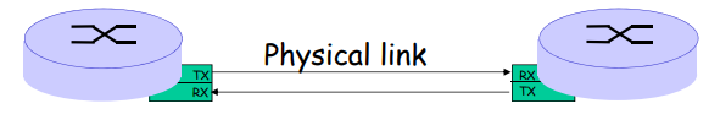
\includegraphics[width=11.899334251607cm,height=2.01961170142988cm]{IIW-Reds-1.pdf}}}}
Nella trasmissione dati attraverso un link fisico si trasmette il
\tmtextbf{bit} tra il trasmittente ( TX ) e il ricevitore ( RX ).

Il physical link {\`e} un link fisico interposto tra TX e RX e pu{\`o} essere:
\begin{itemize}
  \item \tmtextbf{guided media:} i segnali si propagnao tramite un mezzo
  fisico;
  
  \item \tmtextbf{unguided media:} i segnali vengono propagati liberamente
  come nelle onde radio;
\end{itemize}
{\center{\raisebox{0.0\height}{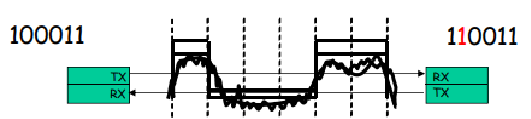
\includegraphics[width=8.92450478814115cm,height=1.99519546110455cm]{IIW-Reds-2.pdf}}}}

In particolare durante la trasmissione su link fisico, la sequenza di bit
(100011) viene utilizzata per modulare la forma d'onda presente nel link che
viene poi ricostruita dall'host ricevente. Tuttavia durante il modulazione
della forma d'onda, il segnale viene soggetto a:
\begin{itemize}
  \item \tmtextbf{attenuazione:} assorbimento energia dall'onda portano a
  un'abbassamento dei picchi dell'onda;
  
  \item \tmtextbf{distorsione}: dovuta alla frequenza di distorsione tipica
  del mezzo su cui viaggia l'onda;
  
  \item \tmtextbf{rumore:} dovuta alle interferenze elettromagnitiche e da
  rumore termico;
  
  \item influenze dal mezzo, bit rate e distanza.
\end{itemize}
Questi fattori portano alla ricezione non corretta della sequenza di bit
invita in partenza ( 110011).

\tmtextbf{Teorema di Shannon}

Un importante risualtato viene fornito dal teorema di Shannon che mette in
correlazione la potenza di trasmissione, la potenza del rumore con il massimo
bandwidth del canale. In particolare, vale la seguente legge:
\[ H \log_2 \left( 1 + \frac{S}{N} \right) \]
In cui:
\begin{itemize}
  \item H:= {\`e} l'intervallo di frequenza su cui il segnale viene trasmesso
  (dipende dal mezzo fisico);
  
  \item $\frac{S}{N} \assign${\`e} il rapporto segnale rumore;
\end{itemize}

\subsubsection{Rete Broadcast}

Una rete \tmtextbf{broadcast} {\`e} una rete in cui in ogni trasmissione tutti
gli host ricevono i segnale. Ne sono un esempio la \tmtextbf{rete wired (
ethernet ) }e la \tmtextbf{rete wireless}:

{\center{\raisebox{0.0\height}{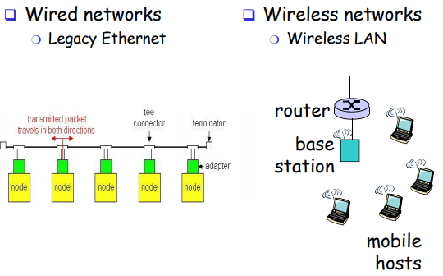
\includegraphics[width=7.4370818575364cm,height=4.62750885478158cm]{IIW-Reds-3.pdf}}}}

\subsubsection{Mezzi fisici}

I mezzi fisici pi{\`u} utilizzati sono:
\begin{itemize}
  \item \tmtextbf{Twisted Pair (TP):} sono formati da due cavi di rame avvolti
  a spirale al fine di aumentare la protezione da interferenze esterne;
  
  \item \tmtextbf{Cavo coassiale:} sono due elementi in rame concentrici usati
  in banda base e banda larga;
  
  \item \tmtextbf{Cavo fibra ottica:} sono cavi formati da fibra di vetro che
  porta la luce pulsante. Ogni pulsazione {\`e} un bit. Il vantaggio risiede
  nel fatto di essere molto veloce e poco affetto da rumore e sono immuni da
  interfeenze elettromagnetiche.
  
  \item \tmtextbf{Radio:} non vi sono cavi, ma si propaga il segnale in
  maniera libera. La radio {\`e} un mezzo non fisico bidirezionale. Lo
  svantaggio consiste nella riflessione del segnale, dall'ostruzione da parte
  di oggetti. Inoltre {\`e} facilmente soggetto ad interferenze.
  
  \ 
\end{itemize}

\subsubsection{Accesso residenziale}

\paragraph{DSL}

L'accesso residenziale pi{\`u} diffuso {\`e} la \tmtextbf{DSL (digital
subscriber line)} e quello via cavo. Questo tipo connessione viene fornito
dalla compagnia telefonica che fornisce il servizio di telefonia fissa,
interpretando di conseguenza un ruoto di ISP.

In particolare, il modem DSL dell'utente utilizza la linea telefonica
esistente per scambiare dati con un \tmtextbf{DSLAM }(Digital Subscriber Line
Access Multiplex) che si trova nella centrale locale della compagnia
telefonica. Il modem DSL residenziale converte i dati digitali in toni ad alta
frequenza per poterli trasmettere alla centrale locale sul cavo telefonico.
Tutti i segnali analogici in arrivo vengono convertiti in formato digitale nel
DSLAM. In aggiunta, la linea telefonica trasportano in parallelo
(contemporaneamente) dati e segnali telefonici in 3 bande di frequenza non
sovrapposte:\tmtextbf{downstream,upstream, canale telefonico}. Tale approccio
fa apparire un singolo collegamento DSL come tre collegamenti separati.

{\center{\raisebox{0.0\height}{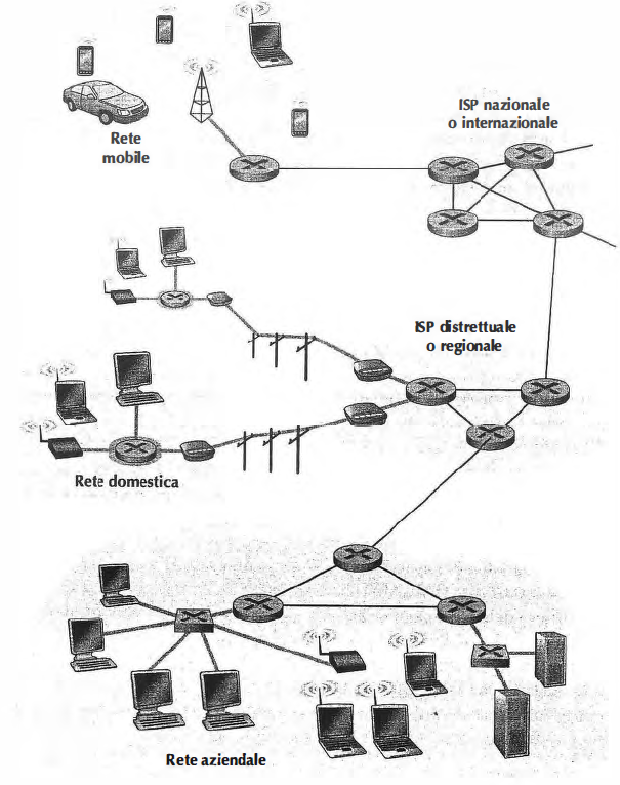
\includegraphics[width=10.4119113210022cm,height=13.1868850846124cm]{IIW-Reds-4.pdf}}}}

Questo accesso viene detto \tmtextbf{asimmetrico} poich{\'e} la velocit{\`a}
di trasmissione in downstram e upstream sono differenti, ma possono essere
anche inferiori perch{\'e} il DSL limita appositamente il tasso di
trasmissione quando offre servizi a pi{\`u} livelli o perch{\'e} il traffico
{\`e} limitato.

\paragraph{Interner via cavo}

Un'altro tipo di \tmtextbf{accesso residenziale} viene fornito
dall'\tmtextbf{accesso ad Internet via cavo}, in cui si utilizzano le
infrastrutture gi{\`a} esistenti della TV. In particolare, un'abitazione
richiede un accesso a Internet via cavo alla stessa azienda che fornisce il
servizio di televisione.

{\center{\raisebox{0.0\height}{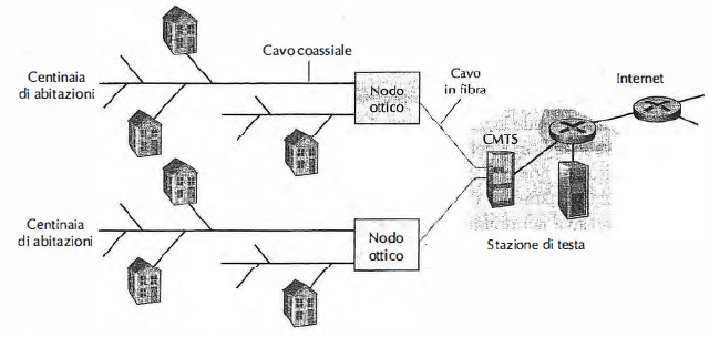
\includegraphics[width=11.899334251607cm,height=5.65217106126197cm]{IIW-Reds-5.pdf}}}}

Si utilizzano fibre ottiche per la terminazione del cavo a giunzioni di
livello di quartiere dalle quali viene usato il tradizionare {\underline{cavo
coassiale}} per la distribuzione televisiva. La connessione vera e provia
viene effettuata tramite il cosiddetto \tmtextbf{cable modem} connesso tramite
le porta Ethernet.

Alla stazione di testa, il sistema di terminazione del cable modem
\tmtextbf{CMTS} traduce il segnale analogico inviato dai cable modem delle
abitazione a valle in formato digitale, similmente al DMSA;inoltre, si divide
la rete HFC in due canali: downstream e upstream. Anch'esso {\`e} asimmetrico.

Una importante caratteristica di quest'ultima soluzione (Americana) {\`e} che
rappresenta un sistema di trasmissione condiviso e ciascun pacchetto inviato
dalla stazione di testa viaggia sul canle di downstram in tutti i collegamenti
e verso ogni abitazione; ciascun pacchetto inviato da un'abitazione viaggia
sul canale di upstream verso la stazione di testa. Per cui se molti utenti
scaricano contemporaneamente, l'effettiva velocit{\`a} sar{\`a} inferiore.

\paragraph{FTTx}

Una tecnlogia che sta prendendo molto piede {\`e} quella del \tmtextbf{fiber
to the home FTTH}, in cui si fornisce fibra ottica dalla centrale locale
direttamente alle abitazioni(FTTH) o il pi{\`u} vicino possibile ad esse
(\tmtextbf{FTTC})-

{\center{\raisebox{0.0\height}{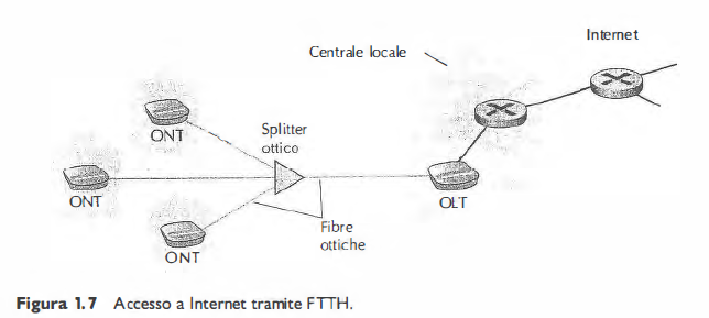
\includegraphics[width=11.899334251607cm,height=5.34607438016529cm]{IIW-Reds-6.pdf}}}}

\

La rete di distribuzione ottica pi{\`u} semplice {\`e} chiamata
\tmtextbf{fibra diretta}, in cui una singola fibra collega una centrale locale
a un'abitazione. In alcuni casi, quando la distanza cabina-abitazione {\`e}
piccola si pu{\`o} ricorrere a cavi singoli in base all'abitazione.

Le architetture utilizzate sono:
\begin{itemize}
  \item \tmtextbf{AON:} sono reti ottiche attive, Ethernet e commutate;
  
  \item \tmtextbf{PON:} sono reti ottiche passive.
\end{itemize}

\paragraph{FTTx - Reti PON}

Nelle reti PON ogni abitazione ha un terminatore ottico chiamato \tmtextbf{ONT
}(Optical Network Terminator) connesso a uno \tmtextbf{splitter} (separatore
ottico) di quartiere tramite una fibra ottica dedicata. Lo splitter combina
pi{\`u} abitazioni in una singola fibra ottica condivisa che si connette a un
altro terminatore che prende il nome di \tmtextbf{OLT }( Optical Line
Terminator) situato nella centrale locale. Quest'ultimo ha la
responsabilit{\`a} di convertire segnali ottici e elettrici e si connette ad
internet tramite un router della compagnia telefonica. Inoltre, tutti i
pacchetti inviati dall'OLT allo splitter sono replicati dallo splitter.

\paragraph{Accesso aziendale}

Nelle aziende per collegarsi ad internet si utilizza una \tmtextbf{rete locale
LAN}. La pi{\`u} diffusa {\`e} la rete Ethernet.

{\center{\raisebox{0.0\height}{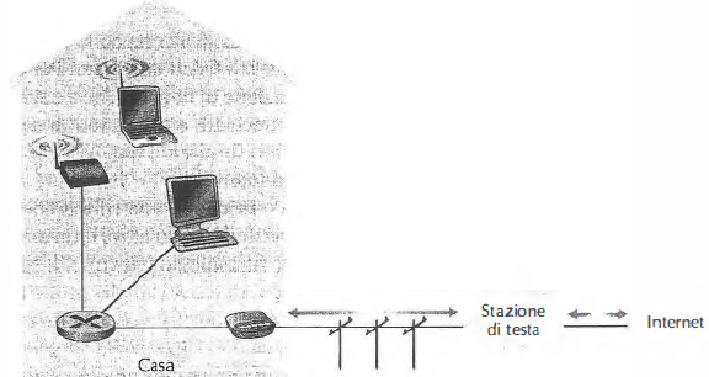
\includegraphics[width=11.899334251607cm,height=6.33528466483012cm]{IIW-Reds-7.pdf}}}}

Ethernet utilizza un doppino di rame intrecciato per collegare numerosi
sistemi periferici tra loro e connetterli a uno swirch. A sua volte, viene
connesso a Internet.

In una LAN wireless, gli utenti trasmettono e ricevono pacchetti da e verso un
access point wireless \tmtextbf{base station} connesso a una rete aziendale
che include una rete Ethernet cablata che a sua volta {\`e} connessa ad
internet.

\paragraph{Accesso Wireless}

Sono tecnlogie che consento di connettersi ad Internet senza l'utilizzo di
alcun cavo. Ve ne sono di due tipologie:
\begin{itemize}
  \item Wifi;
  
  \item Wide Area Wireless Access;
\end{itemize}
La differenza riesce nella portata a cui un dispositivo si pu{\`o} connettere
ad internet.

\subsubsection{Hosts}

Gli Hosth sono i dispositivi che inviano e ricevono dati:
\begin{itemize}
  \item L'applicazione prende i messaggi;
  
  \item L'applicazione divide i messagi in piccole prozioni detti
  \tmtextbf{pacchetti} di lunghezza di L bits;
  
  \item L'applicazione trasmette il pacchetto all'interno della rete di
  accesso a \tmtextbf{velocit{\`a} di trasmissione R}.
  
  \ 
\end{itemize}
\[ \tmop{pck} . \tmop{Trasmission} \tmop{Delay} = \tmop{Time} \tmop{need}
\tmop{to} \tmop{transmit} L \tmop{bit} \tmop{into} \tmop{link} \]
\[ \tmop{pck} \tmop{trasmissione} \tmop{delay} = \frac{L (\tmop{bit})}{R
\left( \frac{\tmop{bit}}{s} \right)} = T_{\tmop{TX}} \]

\subsubsection{Nucleo di rete: Network Core}

Il nucleo della reta {\`e} la parte pi{\`u} interna di una rete. Esso {\`e}
{\underline{una maglia di commutatori di pacchetti e collegamenti che
interconnettono i sistemi periferici di Internet}}.

I dati possono essere trasferiti nella rete tramite due modalit{\`a}:
\begin{itemize}
  \item \tmtextbf{circuit switching:} le risorse vegono dedicare per ogni
  chiamata. es. rete telefonica;
  
  \item \tmtextbf{packet switching:} i dati veongo iviniati tramite porzion
  discrete di bits. Le risorse vengono allocate in base alla richiesta di
  trasmissione dati.
\end{itemize}
{\underline{\tmtextbf{N.B.:}}}

{\center{$\tmop{Switching} \equiv \tmop{Commutazione}$}}
\[ \tmop{Collegamenti} \equiv \tmop{Link} \]

\paragraph{Commutazione a circuito: switching circuit}

Nella commutazione di circuito le risorse richieste lungo un percorso per
consentire la comunicazione tra sistemi periferici sono riservate per l'intera
durata della sessione di comunicazione. {\`e} una connessione end-to-end. In
particolare si riservano:
\begin{itemize}
  \item velcit{\`a} di trasmissione sui collegamenti;
  
  \item buffer di communicazione nei collegamenti
\end{itemize}
Non si ha una condivisione di risorse, ma sono dedicate. Quindi tra una
comunicazione tra ricevitore e tramessitore verranno dedicate 2 linee diverse
in senso opposto.

Il vantaggio di questa commutazione {\`e} che una volta istanziata la
chiamata, si hanno delle prestazioni a circuito, garantite, senza perdita di
dati ne ritardi variabili.

Tuttavia, per garantire la chiamata occorre aspettare un tempo di
\tmtextbf{call setup} in cui si allocano le risorse nelle seguenti fasi:
{\center{\begin{itemize}
  \item \tmtextbf{Call setup} con allocazione di risorse;
  
  \item \tmtextbf{Trasferimento dati} cio{\`e} l'uso delle risorse a
  disposizione;
  
  \item \tmtextbf{Call Teardown} cio{\`e} il rilascio delle risorse;
\end{itemize}}}
Nel caso di una grossa rete a commutazione a circuito in cui bisogna garantire
le risorse necessarie alla comunicazione per ogni utente nella rete e dato che
la capacit{\`a} {\`e} limitata occorre dividere le risorse fra tutti gli
utenti che stanno comunicando. A tale scopo, si deve allocare la capacit{\`a}
trasmissiva tramite \tmtextbf{FDM} (Frequency Division Multiplexing) in cui si
dividono le frequenze disponibili nel link di comunicazione in base agli
utenti che devono usarlo e in misura a quanta frequenza {\`e} necessaria alla
comunicazione. In caso di link totalmente occupato, la comunicazione viene
scartata.
{\center{\raisebox{0.0\height}{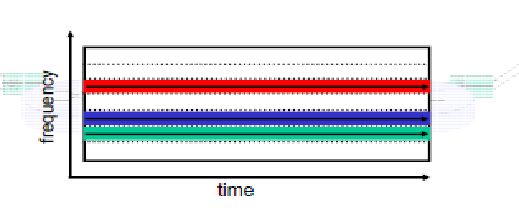
\includegraphics[width=8.71277712186803cm,height=3.48511084874721cm]{IIW-Reds-8.pdf}}}}
Un'altra opzione {\`e} quella di suddividere il link invece che in frequenza,
nel tempo. Questo procedimento viene chiamato \tmtextbf{TDM} (Time Division
Multiplexing) in cui si divide il tempo in slot e ogni slot in frame. Ad ogni
slot di un frame si inserisce una chiamata che verr{\`a} riassegnata al frame
successivo. Questo consente di ottenere un'assegnazione di chiamate del tipo
RR (Round-Robin).

{\center{\raisebox{0.0\height}{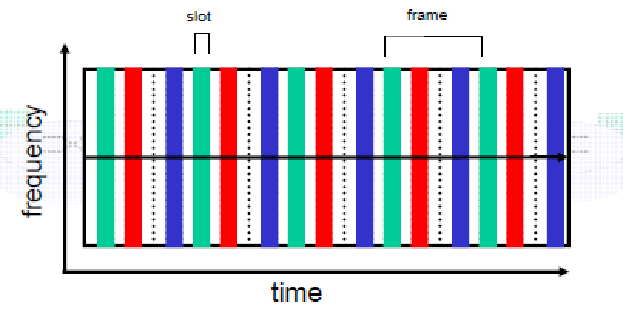
\includegraphics[width=10.4553325462416cm,height=5.22766627312082cm]{IIW-Reds-9.pdf}}}}

Il grande svantaggio di una commutazione a circuito di tipo TDM {\`e} che
l'assegnazione viene fatta ad ogni frame e cquindi si possono riscontrare
\tmtextbf{periodi di silenzi}.

\paragraph{Commutazione a pacchetto: packet switching}

{\center{\raisebox{0.0\height}{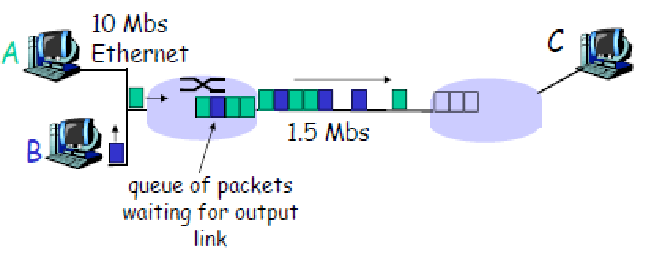
\includegraphics[width=10.9780926144563cm,height=4.25183654729109cm]{IIW-Reds-10.pdf}}}}

L'applicazione distribuite scambiano \tmtextbf{informazioni}. Queste
informazioni in ogni stream end-to-end vengono divisi in \tmtextbf{pacchetti}
contentneti dati.

Nella rete LAN le risorse vengono \tmtextbf{condivise} (dagli Host al Router)
ed ogni pacchetto utilizza il massimo della capacit{\`a} del link.

La commutazione {\`e} di tipo \tmtextbf{store-and-forward} cio{\`e} il
commutatore deve ricevere l'intero pacchetto prima di poterne cominciare a
trasmettere sul collegamento in uscita il primo bit.In particolare:
{\center{\raisebox{0.0\height}{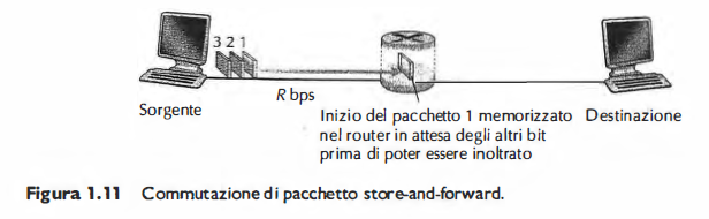
\includegraphics[width=11.899334251607cm,height=3.68311360356815cm]{IIW-Reds-11.pdf}}}}
In questo esempio la rete {\`e} costituita da 2 sistemi periferici e un
router. Il router di norma {\`e} dotato di molti collegamenti e la sua
funzione {\`e} quella di instradare un pacchetto in entrato su un collegamento
in uscita. Il ruoter non pu{\`o} trasmettere i bit che ha ricevito finch{\'e}
non ha immagazzinato nel suo buffer tutte i bit del pacchetto arrivatogli. Una
volta ricevuti, pu{\`o} iniziare a trasmettere in uscita.

{\center{\raisebox{0.0\height}{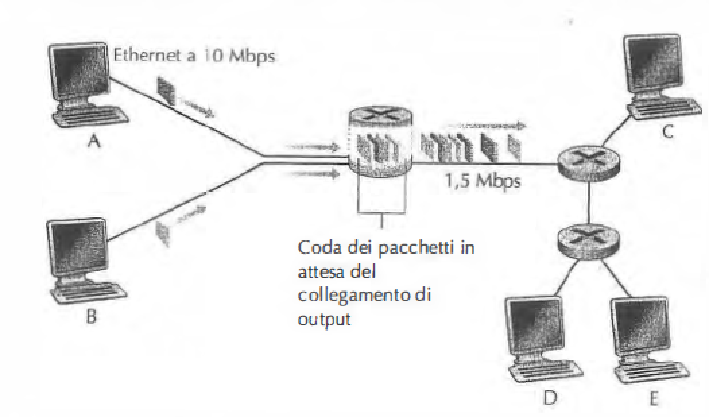
\includegraphics[width=11.899334251607cm,height=7.00670667716122cm]{IIW-Reds-12.pdf}}}}

Se pensiamo ad una rete con pi{\`u} collegamenti, il commutatore deve mantenre
per ogni collegamento un \tmtextbf{buffer di output} per conservare i
pacchetit che sta per inviare su quel collegamento. Se un pacchetto in arrivo
richiede l'invio attraverso un collegamento, ma questo {\`e} occupato da
un'altra trasmissione, quello in arrivo deve attendere nel \tmtextbf{buffer di
output}. Di conseguenza, oltre ai ritardi store-and-forward, i pacchetti
subiscono anche \tmtextbf{ritardi di accodamento} nei buffer di output.

In particolare, questi ritardi sono variabili e dipendono dal livello di
traffico nella rete e quindi un pacchetto in arrivo pu{\`o} trivare il buffer
ocmpletamento pieno da altri pacchetti comportando, di conseguenza, la
\tmtextbf{perdita del pacchetto}. Da questa caratteristica la commutazione a
pacchetto prende il nome di \tmtextbf{multiplazione statistica} data
dall'assenza di un pattern fissato dei pacchetti messi in cosa al router.

{\center{\raisebox{0.0\height}{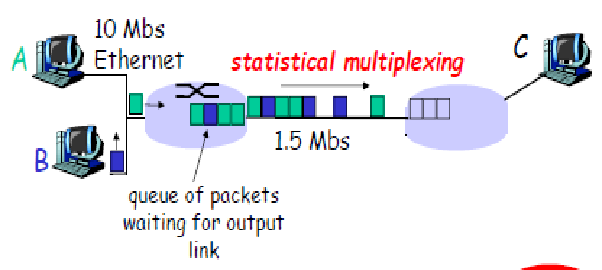
\includegraphics[width=10.1068149022694cm,height=4.53064738292011cm]{IIW-Reds-13.pdf}}}}

\paragraph{Router}

Nelle reti LAN con commutazione a pacchetto, ogni pacchetto che percorre la
rete contiente nella propria intestazione l'indirizzo della sua destinazione
che presenta una struttura gerarchica. Questo pacchetto deve attraversare i
cosiddetti \tmtextbf{router} che esamina una parte dell'indirizzo di
destinazione e lo inoltra al collegamento opportuno (\tmtextbf{next hop}).

Per fare ci{\`o} il route possiede una \tmtextbf{tabella di inolto/forwarding
table} che mette in relazione gli indirizzi di destinazione con i collegamenti
in uscita.

Il processo di calcolo e mantenimento della tabella di routing viene detta
\tmtextbf{routing}.
{\center{\begin{figure}[h]
  \raisebox{0.0\height}{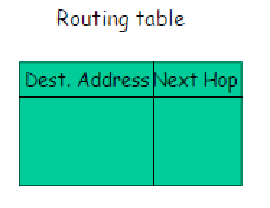
\includegraphics[width=4.53064738292011cm,height=3.48511084874721cm]{IIW-Reds-14.pdf}}
  \caption{}
\end{figure}}}

\paragraph{Commutazione a pacchetto vs Commutazione a circuito}

\begin{itemize}
  \item la commutazione a pacchetto, apparentemente, non {\`e} adatta a
  servizi in tempo reale a causa dei ritardi end-to-end variabili e non
  determinabili a priori. Tuttavia, la commutazione a pacchetto fornisce una
  migliore condivisione della larghezza di banda rispetto alla commutazione a
  circuito, {\`e} pi{\`u} semplice,efficiente e meno costosa.
  
  \item La commutazione a pacchetto {\`e} pi{\`u} efficiente poich{\'e} le
  risorse che consentono il collegamento nella rete avvengono a richiesta e
  non garantita come la commutazione a pacchetto in cui vengono riservate.
  Quindi, nel caso in cui la rete non {\`e} congestionata i singoli pacchetti
  viaggeranno al massimo; se non {\`e} congestionata i pacchetti verranno
  messi in coda o persi e quindi si svilupperanno dei ritardi.
  Complessivamente andr{\`a} pi{\`u} ``veloce'' la commutazione a pacchetto e
  quindi sar{\`a} pi{\`u} efficiente;
  
  \ 
\end{itemize}

\paragraph{Packet switching vs Message switching}

{\center{\begin{figure}[h]
  \raisebox{0.0\height}{
\includegraphics[width=6.97022169749443cm,height=1.39403778040142cm]{IIW-Reds-15.pdf}}
  \caption{
  }
\end{figure}}}
Un pacchetto {\`e} una porzione piccola di dati da trasmettere. Un messaggio
{\`e} l'intero dato che deve essere scambiato da una applciazione.

Si ha un'efficienza maggiore nella trasmissione a pacchetto.

Ipotizziamo che abbiamo una rete che trasmette messaggi L nella rete sopra in
figura. Il percorso di rete prevede 3 link con2 router ed effettuer{\`a} 3
next hop.

Ogni trasmissione ha un ritardo $\frac{L}{R}$ e moltiplicati per 3 link
otteniamo $3 \frac{L}{R}$.

Se utilizzassimo la commutasione a pacchetto: il messaggio viene diviso in
tanti pacchetti ed inoltrati nei vari collegamenti [\tmtextbf{message
segmenting}]. In questo caso, l'invio e l'arrivo dei pacchetti avviene in
maniera continua poich{\`e} appena il router riceve l'ultimo bit del pacchetto
lo spedisce subito e, nel frattempo, gliene arriva un'altro dal link di
arrivo. Quindi ogni link lavora in parallelo.

Questa tecnica viene detta \tmtextbf{pipeline}.

\paragraph{Virtual Circuit Network}

Nella commutazione a pacchetto vi siono varie tipologie di organizzazione
della rete.

{\center{\begin{figure}[h]
  \raisebox{0.0\height}{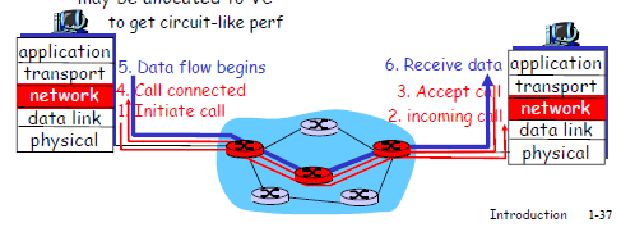
\includegraphics[width=10.4119113210022cm,height=3.79391315754952cm]{IIW-Reds-16.pdf}}
  \caption{}
\end{figure}}}

La \tmtextbf{rete a circuito virtuale} {\`e} un tipo di rete che utilizza una
\tmtextbf{commutazione a pacchetto}, ma a livello logico, cio{\'e} virtuale,
si ha una \tmtextbf{commutazione a circuito}.In particolare,si ha una
allocazione di risorse a livello logico.In cui:
\begin{itemizearrow}
  Si stabilisce una connessione del tipo:
  \begin{itemize}
    \item Call setup: in cui si trova un cammino tra i router:
    
    \item Allocazione di link,banda e buffer in maniera virtuale per ottenere
    un circuito;
    
    \item Si trasferiscono dati in cui ogni pacchetto porta un identificatore
    virtuale;
    
    \item Si chiude la connessione (Teardown);
  \end{itemize}
\end{itemizearrow}

\paragraph{Datagram Network - Rete a datagramma}

La \tmtextbf{rete a datagramma} {\`e} un tipo di organizzazione di rete a
pacchetto, utlizzato in Internet.

In particolare, {\`e} una rete a pacchetot in cui non si ha il concetto di
connessione, i router non hanno nozione di connessione tra utenti. I pacchetti
vanno da un nodo sorgente-destinazione e vengono instradati tramite il loro
indirizzo host. Questo instradamento non {\`e} univoco.

{\center{\begin{figure}[h]
  \raisebox{0.0\height}{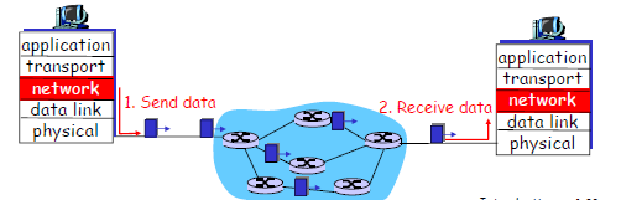
\includegraphics[width=10.4119113210022cm,height=3.35063295290568cm]{IIW-Reds-17.pdf}}
  \caption{}
\end{figure}}}

\subsubsection{Struttura di Internet: una reti di reti}

L'obiettivo {\`e} quello di interconnettere gli \tmtextbf{ISP} (Internet
Service Provider) di accesso in moodo che i sistemi periferici possano
scambiarsi pacchetti.

L'idea pi{\`u} semplice consisterebbe nell'interconnettere tutti gli ISP di
accesso con un \tmtextbf{unico ISP globale di transito}. Questo \tmtextbf{ISP
globale} {\`e} una rete di router e collegamenti che copre l'intero globo, ma
ha anche almeno un router prossimo a ognuno delle ISP di accesso.

{\center{\begin{figure}[h]
  \raisebox{0.0\height}{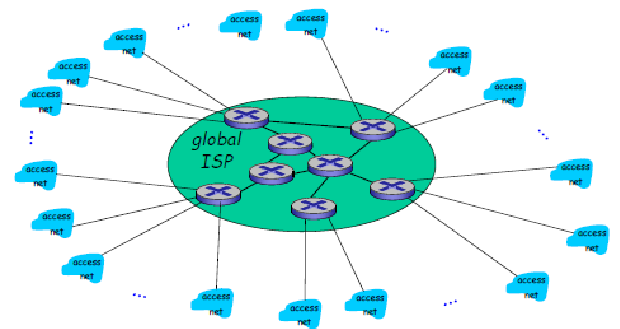
\includegraphics[width=10.4119113210022cm,height=5.53220516856881cm]{IIW-Reds-18.pdf}}
  \caption{}
\end{figure}}}

Questa soluzione risulterebbe molto costosa e non praticabile. Un'alternativa
consisterebbe in centinaia di migliia di ISP di accesso e pi{\`u} ISP globali.
Tuttavia, anche in questa ipotesi gli ISP globali devono essere connessi tra
di loro e ci potrebbero essere ISP che non comunicano.

Questa struttura di rete {\`e} formata da una \tmtextbf{gerarchia} a due
livelli in qui i provider globali di transito stanno in cima alla gerachia e
gli ISP di accesso stanno alla base.

{\center{\begin{figure}[h]
  \raisebox{0.0\height}{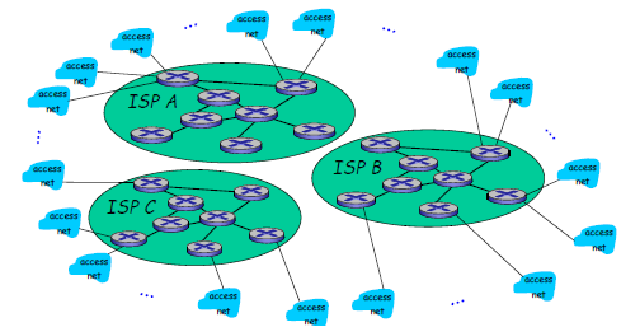
\includegraphics[width=10.4119113210022cm,height=5.47546897546898cm]{IIW-Reds-19.pdf}}
  \caption{}
\end{figure}}}

Questa caratterizzazione della rete, tuttavia, implica che ogni ISP globale
sia prossima ad ogni ISP di accesso. Inutile dire che questa soluzione non
pu{\`o} essere applicabile. A tale scopo, si introducono gli \tmtextbf{ISP
regionali} al quale si connettono tutti gli ISP di accesso: ogni ISP regionale
si connette all'\tmtextbf{ISP di primo livello}.

{\center{\begin{figure}[h]
  \raisebox{0.0\height}{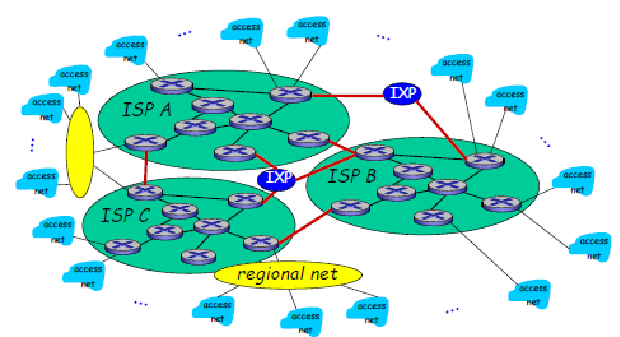
\includegraphics[width=10.4119113210022cm,height=5.66110783156238cm]{IIW-Reds-20.pdf}}
  \caption{}
\end{figure}}}

In questa nuova gerarchia ogni ISP di accesso paga l'ISP regionale a cui si
connette che paga il suo ISP di primo livello, ma pu{\`o} accadere anche che
un ISP di accesso si colleghi direttamente con un ISP di primo livello.
Inoltre, in una gerarchia di rete di questa tipologia vi possono essere
offerti dei servizi del tipo:
\begin{itemize}
  \item \tmtextbf{POP:} esistono in tutti i livelli della gerarchia tranne
  negli ISP di accesso. Esso {\`e} un gruppo di router vicini tra loro nella
  rete del providere, tramite il quale gli ISP clienti possono connettersi al
  fornitore.;
  
  \item \tmtextbf{Multi-homing}: qualunque ISP, tranne di primo livello,
  pu{\`o} scegliere la modalita di connettersi a pi{\`u} ISP fornitori.
  
  \item \tmtextbf{Peering}: per diminuire il costo pagato all'ISP fornitore,
  una coppia di ISP di pari livello gerarchico pu{\`o} fare uso di
  \tmtextbf{peering}, cio{\'e} si connettono i due ISP al fine di stabilire
  una connessione diretta di traffico senza transitare per un intermediario.
  Utilizzando queste connessioni un'azienda terza pu{\`o} creare un
  \tmtextbf{IXP}, cio{\`e} un punto d'incontro in cui pi{\`u} ISP fanno
  peering tra di loro.
\end{itemize}
Tutt'ora la situazione {\`e} quella descritta di sopra con l'aggiunta di reti
che si occupano di distribuire i contenuti:
{\center{\begin{figure}[h]
  \raisebox{0.0\height}{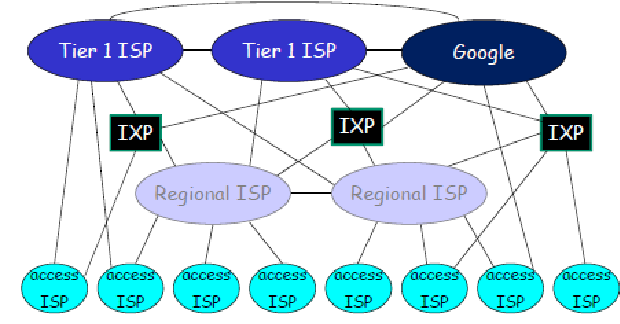
\includegraphics[width=10.4119113210022cm,height=5.43629476584022cm]{IIW-Reds-21.pdf}}
  \caption{}
\end{figure}}}


\

\subsubsection{Ritardi, perdite e throughput nelle reti a commutazione di
pacchetto}

Ricordiamo che un pacchetto parte da un host (sorgente), passa attraverso una
serie di router e conclude il viaggio in un altro host. In ogni tappa il
pacchetto subisce vari tipi di ritardo a ciascun nodo del tragitto. I
principali ritardi sono:

\tmtextbf{\begin{itemize}
  \item ritardo di elaborazione;
  
  \item ritardo di accodamento;
  
  \item ritardo di trasmissione;
  
  \item ritado di propagazione;
\end{itemize}}

Complessivamente formano il \tmtextbf{ritardo totale di nodo.}

\begin{figure}[h]
  \raisebox{0.0\height}{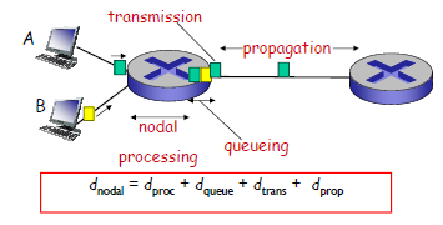
\includegraphics[width=7.4370818575364cm,height=3.77444903581267cm]{IIW-Reds-22.pdf}}
  \caption{}
\end{figure}

In particolare quando il pacchetto arriva al router A dal note a monte, il
router ne esamina l'intestazione per determinare il collegamento in uscita
appropriato e quindi dirige il pacchetto su tale collegamento. Un pacchetot
pu{\`o} essere trasmesso su un collegamento solo se non ci sono altri
pacchetti in fase di trasmissione e se non esistono pacchetti ch elo precedono
nella coda; se il collegamento {\`e} momentaneamente occupato o se altri
pacchetto sono accordati, l'ultimo pachetto arrivato si metter{\`a} anch'esso
in coda.

\paragraph{Ritardo di elaborazione}

Il \tmtextbf{ritardo di elaborazione} {\`e} il tempo richiesto per esaminare
l'intestazione del pacchetto e per determinare dove dirigerlo. Pu{\`o}
includere il tempo necessario per controllare errori a livello di bit.

Nei router ad alta velocit{\`a} questi ritardi sono nell'ordine dei $\mu s$.

\paragraph{Ritardo di accodamento}

Una volta in coda, il pacchetot subisce un \tmtextbf{ritardo di accodamento
(queuing delay)} mentre attende la trasmissione sul collegamento. Questo
ritardo dipende dal numero di pacchetti precedentemente arrivati, accodati e
in attesa di trasmissione sullo stesso colelgamento.

Se la cosa {\`e} vuota e non {\`e} in corso la trasmissione di altri
pacchetti, allora il ritardo di accodamento del pacchetto sar{\`a} nullo. Se
il traffico {\`e} pesanti e molti altri pacchetti stanno aspettando la
trasmissione questo ritardo sar{\`a} pi{\`u} lungo.

\paragraph{Ritardo di trasmissione}

Assumendo che la trasmissione dei pacchetti sia di tipo \tmtextbf{FIFO}, il
pacchetto sar{\`a} trasmesso solo dopo la trasmissione di tutti i pacchetti
che lo hanno preceduto nell'arrivo.

Se:
\begin{itemizeminus}
  \item $L$:= lunghezza pachetto in bit;
  
  \item R:= velocit{\`a} di trasmissione del collegamento in bps;
\end{itemizeminus}
Il \tmtextbf{ritardo di trasmissione} {\`e}: $\frac{L}{R}$. Coincide con il
tempo necessario a trasmettere tutti i bit del pacchetto sul collegamento.

\paragraph{Ritardo di propagazione}

Un volta immesso sul collegamento, un bit deve propagarsi fino al router B.

Il tempo impiega alla propagazione del bit {\`e} detto \tmtextbf{ritardo di
propagazione}. Il bit viaggia alla velocit{\`a} di propagazione del
collegamento che dipende dal mezzo fisico (velocit{\`a} della luce) e dalla
lunghezza dello stesso.

Il \tmtextbf{ritardo di propagazione} {\`e}:$\frac{d}{v}$ $v = 3 \times 10^8
\frac{m}{s}$

\paragraph{Ritardo trasmissione vs Ritardo propagazione}

Il ritardo di trasmissione {\`e} la quantit{\`a} di tempo rischiesta da parte
del router per trasmettere in uscita il pacchetto e, quindi, indipendente
dalla distanza tra i router.

Il ritardo di propagazione {\`e} il tempo richiesto per la propagazione di un
bit da un router a quello successivo e,quindi indipendente dalla lunghezza del
pacchetto e dalla velocit{\`a} propria del collegamento.

\paragraph{Ritardo di accodamento e perdita dei pacchetti}

La componente pi{\`u} complessa del ritardo totale del nodo {\`e} il
\tmtextbf{ritardo di accodamento}. Per essere rigorosi bisognerebbe introdurre
concetti di multiplazione statistica e \tmtextbf{coda M/M/n}.

In maniera semplicistica, assumiamo che:

$\begin{itemizeminus}
  \item  L a \frac{\tmop{bit}}{s} \assign \tmop{velocit} {\`a} \tmop{media}
  \tmop{di} \tmop{arrivo} \tmop{dei} \tmop{bit} \tmop{in} \tmop{coda} ;
  
  \item  \tmop{Coda} \tmop{molto} \tmop{grande} \tmop{per} \tmop{avere}
  \tmop{un} \tmop{numero} \tmop{illimitato} \tmop{di} \tmop{bit} ;
  
  \item  \frac{\tmop{La}}{R} \assign \tmmathbf{\tmop{Intensit} {\`a} \tmop{di}
  \tmop{traffico}}
\end{itemizeminus}$

Quindi:
\begin{itemizeminus}
  \item Se $\frac{La}{R} > 1$, la velocit{\`a} media di arrivo dei bit nella
  cosa supera la velcoit{\`a} alla quale i bit vengono ritrasmessi in
  uscita$\rightarrow$la coda tender{\`a} a crescere senza lmiti e il ritardo
  di coda tender{\`a} all'infinito.
  
  \item Se $\frac{La}{R} \leqslant 1$, la natura del traffico in arrivo
  influisce sul ritardo in coda. In particolare se i pacchetti arrivano con
  scadenza periodica (L/R), allora la coda sar{\`a} sempre vuota e la
  ritrasmissione avviene senza ritardi. Se i pacchetti arrivano a raffiche
  periodiche si possono verificare ritardi medi di accodamento.
\end{itemizeminus}
{\center{\begin{figure}[h]
  \raisebox{0.0\height}{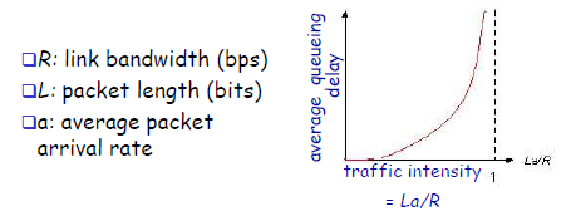
\includegraphics[width=9.66820805457169cm,height=3.54125672307491cm]{IIW-Reds-23.pdf}}
  \caption{}
\end{figure}}}

\paragraph{Perdita di pacchetti}

Poich{\'e} la capacit{\`a} della coda {\`e} finita, i ritardi dei pacchetti
non tengono all'infinito quando l'intensit{\`o} di traffico si approssima a 1,
ma un pacchetot pu{\`o} trovare la coda piena. In questo caso, il router
eliminer{\`a} il pacchetto. Questa frazione di pacchetti persi aumenta con
l'aumentare del traffico.

Dal punto di vista dei sistemi periferici, la perdit{\`a} sembrer{\`a} come se
il pacchetto fosse stato inviato in rete, ma non fosso pi{\`u} riemerso alla
destinazione.

\subsubsection{Throughput}

Il \tmtextbf{throughput} {\`e} la velocit{\`a} in cui si i bit sono trasferiti
fra la sorgente e la destinazione. Pu{\`o} essere due tipi:
\begin{itemize}
  \item \tmtextbf{instanstaneo:} {\`e} la velocit{\`a} di trasferimento in un
  determinanto tempo;
  
  \item \tmtextbf{medio:} {\`e} la velocit{\`o} di trasferimento in periodo di
  tempo pi{\`u} lungo;
\end{itemize}
Consideriamo il throughtput per u trasferimento di file da server e clinet.
Definiamo:
\begin{itemizeminus}
  \item $R_s$ velocit{\`a} del collegamento tra server e router;
  
  \item $R_c$ velocit{\`a} del collegamento tra server e client;
\end{itemizeminus}
Se:
\begin{itemizeminus}
  \item $R_s < R_c \rightarrow$ i bit immessi dal server scorreranno
  attraverso il router e arriveranno al cliente a una velocit{\`a} $R_s$ dando
  un \tmtextbf{throughput} di $R_s$bps;
  
  \item $R_c < R_s \rightarrow$il router non sar{\`o} in grado inoltrare bit
  alla stessa velocit{\`a} alla quale li riceve. I bit lasceranno il router ad
  una velocit{\`a} $R_c$ danto un \tmtextbf{throughput} end-to-end di $R_c$.
\end{itemizeminus}
Quindi da queste considerazioni, il \tmtextbf{throughput} in una rete {\`e}
dato da:
\[ \tmop{Thr} = \min (R_s, R_c, k) \tmop{dove} k {\`e} \tmop{il} \tmop{rate}
   \tmop{del} \tmop{collegamento} \tmop{condiviso} \]
In pratica {\`e} la velocit{\`a} di trasmissione del collegamento che fa da
\tmtextbf{collo di bottiglia} (bottleneck).
{\center{\begin{figure}[h]
  \raisebox{0.0\height}{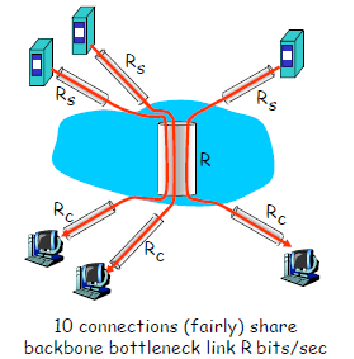
\includegraphics[width=5.94965892693165cm,height=6.0346484323757cm]{IIW-Reds-24.pdf}}
  \caption{}
\end{figure}}}

\section{Livelli dei protocolli e loro modelli di servizio}

Un'architettura a livelli consente di discurete una parte specifica e ben
definita di un sistema articolato e complesso. A tale scopo si introduce il
concetto di \tmtextbf{modularit{\`a}} che consente lo sviluppo, la
manutenzione, e la modifica dell'implementazione del servizio di un
determinato livello in maniera facile.Infatti,finch{\'e} il livello fornisce
lo stesso servizio allo strato superiore e utilizza gli stessi servizi dello
strato inferiore, la parte rimanente del sistema rimane invariata.

Nei sistemi di rete l'obiettivo {\`e} quello di instaurare una comunicazione.
A tale scopo si stratificano tutti i protocolli che consensono la
comunicazione in strati ordinati che implementano un sottoinsieme di tutte le
funzionalit{\`a} necessarie all'adempimento di un determinato
\tmtextbf{servizio.}Quindi un \tmtextbf{servizio} {\`e} un insieme di funzioni
offerte al livello superiore (come per esempio \tmtextbf{flow control,error
control}) che d'altro canto dipender{\`a} dai servizi offerti dal livello
inferiore. Risultando che ogni livello fornisce un valore aggiunto a livello
di comunicazione rispetto al livello inferiore.

All'interno di ogni livello ci sono le \tmtextbf{entit{\`a}} che svolgono le
attivit{\`a} del livello.

Se immaginiamo ad un'architettura di rete stratificata, essa sar{\`a} formata
da \tmtextbf{N-Layers} che forniranno \tmtextbf{N-Service}, implementato da
\tmtextbf{N-entity}. La struttura sar{\`a} la seguente:

{\center{\begin{figure}[h]
  \raisebox{0.0\height}{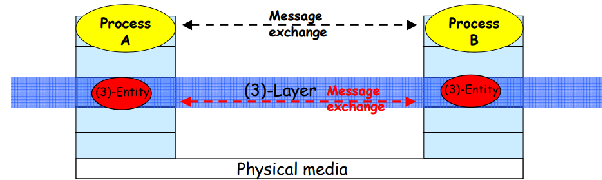
\includegraphics[width=10.1144234553325cm,height=3.02567886658796cm]{IIW-Reds-25.pdf}}
  \caption{}
\end{figure}}}

Tipicamente lo strato pi{\`u} alto {\`e} lo strato dell'applicazione. Esso e
distribuito e presente in tutti gli end-system che si devono interfacciare
alla reta; mentre lo strato pi{\`u} basso {\`e} rappresentato dal mezzo fisico
che consente l'effettivo trasporto nella rete dei messaggi.

Gli svantaggi della stratificazione a livelli sono che:
\begin{itemize}
  \item un livello potrebbe duplicare le funzionalit{\`a} del livello
  sottostante;
  
  \item La funzionalit{\`a} di un livello potrebbe aver bisogno di
  informazioni presenti solamente in un altro livello, entrando di conseguenza
  in contraddizione con l'obiettivo che ci eravamo prefissati.
\end{itemize}


\subsection{Entit{\`a}}

Le \tmtextbf{entit{\`a}} hanno la responsabilit{\`a} di realizzare il servizio
e per adempire a tale scopo necessitano la cooperazione con le altre
entit{\`a} dello stesso livello, scambiandosi dei \tmtextbf{messaggi}
attraverso i servizi di comunicazione forniti dai livelli sottostanti.

\subsection{Servizi}

{\center{\begin{figure}[h]
  \raisebox{0.0\height}{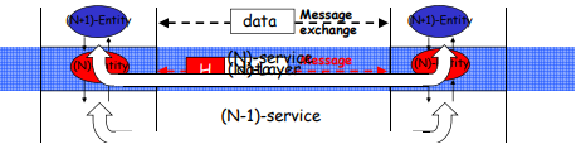
\includegraphics[width=9.66820805457169cm,height=2.39590712317985cm]{IIW-Reds-26.pdf}}
  \caption{}
\end{figure}}}

Per realizzare un \tmtextbf{servizio}, l'iter con cui procedere {\`e} il
seguente:
\begin{itemize}
  \item (N)-Livello fornisce il (N)-servizio alle (N+1)-entit{\`a} che
  consiste nella realizzazione di (N)-funzioni;
  
  \item Le (N)-funzioni scolte dalle (N)-enit{\`a} richiedono (N-1)-servizi,
  richiedendo la cooperazione delle (N)-entit{\`a} del secondo sistema.
\end{itemize}
Inoltre, i servizio possono essere di due tipologie:
\begin{itemize}
  \item \tmtextbf{Connection Oriented (N)-Service} in cui, per comunicare, gli
  (N)-utenti devono:
  \begin{itemize}
    \item Instaurare una connessione;
    
    \item Trasferire i Dati;
    
    \item Terminare la connessione;
  \end{itemize}
  \item \tmtextbf{Connectionless (N)-Service}: si ha il semplice trasferimento
  dei dati.
\end{itemize}

\subsection{(N)-Protocol}

Al fine di gestire la cooperazione tra le (N)-entit{\`a} si utilizzano i
\tmtextbf{protocolli}. Essi hanno la responsabilit{\`a} di gestire:
\begin{itemize}
  \item Sintassi dei tipi di messaggi, specificando come sono delineati i
  campi dei messaggi e come sono fatti;
  
  \item Semantica dei campi cio{\`e} il significato del messaggio che si sta
  ricevendo;
  
  \item Regole per come e quando i processi inviano e rispondono ai messaggi.
\end{itemize}
Ogni protocollo appartiene ad un libello.

\subsection{Protocol Data Unit (PDU)}

Il \tmtextbf{protocol data unit} {\`e} un protocollo che governa i messaggi
strambiati tra le (N)-entit{\`a} rappresentando l'effettiva informazione che
attraversa i livelli dell'architettura a strati. Essa comprende i
\tmtextbf{dati dell' (N)-Servizio} e tipicamente un \tmtextbf{header} utile
allo svolgimento delle N-funzioni.

{\center{\begin{figure}[h]
  \raisebox{0.0\height}{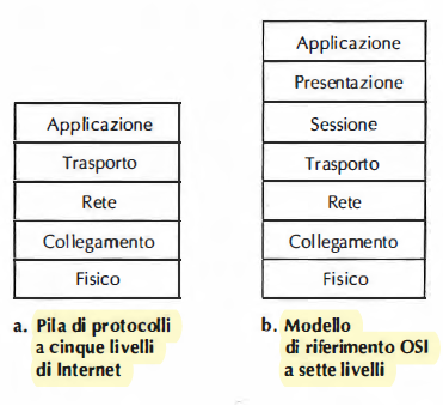
\includegraphics[width=7.4370818575364cm,height=6.79502820411911cm]{IIW-Reds-27.pdf}}
  \caption{}
\end{figure}}}

\subsection{Modello OSI}

I principi del \tmtextbf{modello OSI} ( Open System Interconnection) sono i
seguenti:
\begin{itemize}
  \item Minimizzare il numero dei livelli;
  
  \item Stabilire dei confini nel quale avvengono le interazioni minime;
  
  \item I livelli dovrebbero implementare differenti funzioni;
  
  \item I livelli dovrebbere essere reimplementati senza modificale le
  interfacce con i livelli adiacenti;
  
  \item Ogni livello dovrebbe fornire un valore aggiunto.
\end{itemize}
Inotre, presenta la seguente struttura:
{\center{\begin{figure}[h]
  \raisebox{0.0\height}{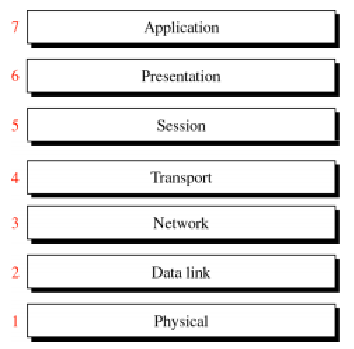
\includegraphics[width=5.94965892693165cm,height=5.85571625344353cm]{IIW-Reds-28.pdf}}
  \caption{}
\end{figure}}}
\tmtextbf{Application Layer}

L'\tmtextbf{application layer} {\`e} dove le applicazioni di rete e i loro
protocolli risiedono. Un esempio di protocollo di applicazione {\`e} il
protocollo HTTP.

Un protocollo di quello livello {\`e} distribuito su molteplici end-system
con consentono, attraverso i layer inferiori ( sotto analizzati), di scambiare
pacchetti con altri end-system. Questi pacchetti vengono detti
\tmtextbf{messaggi}.

\tmtextmd{\tmtextbf{Presentation Layer}}

Il \tmtextbf{presentation layer} gestisce la semantica e la sintassi delle
informazioni scambiate rendendo indipendente la codifica dei messaggi
indipendente dalla comunicazione. Ha la responsabilit{\`a}, quindi, di
tradurre,decifrare e comprimere i dati.

\tmtextbf{Session Layer}

Il \tmtextbf{session layer} permette di gestire la sessione. In particolare
fornisce la delimitazione e la sincroizzazione dello scambio di dati, compresi
i mezzi per costruire uno schema di controllo e recupero degli stessi.

\tmtextbf{Transport Layer}

Il \tmtextbf{transport layer} trasporta i messaggi del \tmtextbf{application
layer} tra gli end point. Ha la responsabilit{\`a} di indirizzamento
indirizzo-punto; segmentazione e riassemplamento, controllo di connessione,
controllo di flusso, controllo di errori, controllo di congestione.

\tmtextbf{Network Layer}

Il \tmtextbf{network layer} consente la consegna dei pacchetti dalla sorgente
alla destinazione. Ha la responsabilit{\`a} di indirizzamento logico e di
routing.

\tmtextbf{Data link layer}

Il \tmtextbf{data link layer} trasforma il \tmtextbf{physical layer} in un
link affidabile tramite:
\begin{itemize}
  \item frammentazione;
  
  \item Addressing fisico;
  
  \item flow control;
  
  \item error control;
  
  \item Access control ( Importante nelle connessioni Broadcast);
\end{itemize}
\tmtextbf{Physical Layer}

Il \tmtextbf{physical layer} coordina le funzioni richieste per trasmettere i
bit su un link fisico. Definisce:
\begin{itemize}
  \item Le caratteristiche delle interfacce e del mezzo;
  
  \item Rappresentazione Bit;
  
  \item Velocit{\`a} di trasmissione;
  
  \item Sincronizzazione del bit;
  
  \item Configurazione di linea, modalit{\`a} di trasmissione etc{\textdots}
\end{itemize}
Non tutti i dispositivi hanno nella loro architettura tutti i 7 livelli del
modello OSI: quelli necessari per la connessione sono i primi 3 ( tipicamente
posseduti dai router/ switch), mentre gli end systems li posseggono tutti.

Quello che si verifica nella realt{\`a} {\`e} una sorta di
\tmtextbf{incapsulamento} in cui ogni livello aggiunge/toglie gli
header/identificativi del livello precedente/successivo per permettere alle
N-entit{\`a} di svolgere l'N-servizio costituito dall'N-funzioni per cooperare
a sua volta con le N+1 entit{\`a}. Graficamente:
{\center{\begin{figure}[h]
  \raisebox{0.0\height}{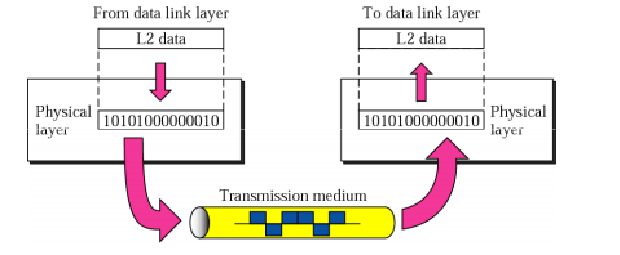
\includegraphics[width=10.4119113210022cm,height=4.28045060999606cm]{IIW-Reds-29.pdf}}
  \caption{}
\end{figure}}}
{\center{\begin{figure}[h]
  \raisebox{0.0\height}{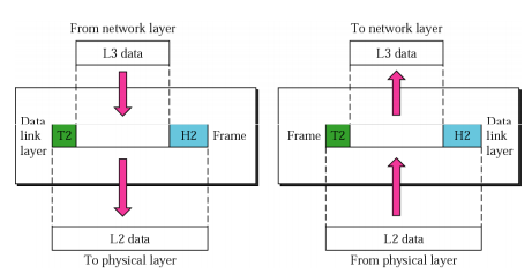
\includegraphics[width=8.92450478814115cm,height=4.56541059950151cm]{IIW-Reds-30.pdf}}
  \caption{}
\end{figure}}}

{\center{\begin{figure}[h]
  \raisebox{0.0\height}{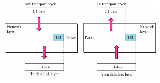
\includegraphics[width=2.68485176439722cm,height=1.3992686606323cm]{IIW-Reds-31.pdf}}
  \caption{}
\end{figure}}}

{\center{\begin{figure}[h]
  \raisebox{0.0\height}{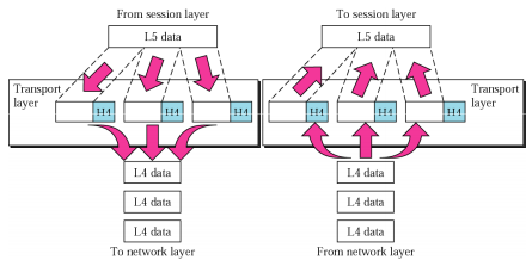
\includegraphics[width=8.92450478814115cm,height=4.46225239407058cm]{IIW-Reds-32.pdf}}
  \caption{}
\end{figure}}}

{\center{\begin{figure}[h]
  \raisebox{0.0\height}{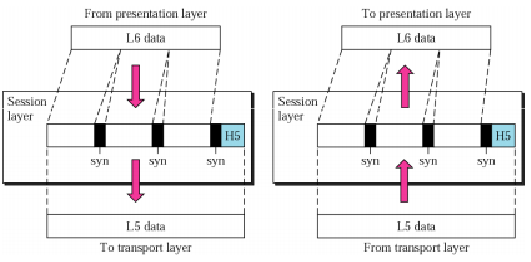
\includegraphics[width=8.92450478814115cm,height=4.39229961957235cm]{IIW-Reds-33.pdf}}
  \caption{}
\end{figure}}}

{\center{\begin{figure}[h]
  \raisebox{0.0\height}{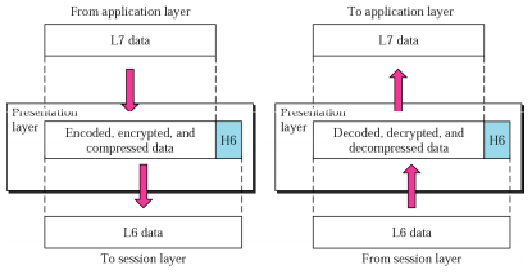
\includegraphics[width=8.92450478814115cm,height=4.59138462547554cm]{IIW-Reds-34.pdf}}
  \caption{}
\end{figure}}}

{\center{\begin{figure}[h]
  \raisebox{0.0\height}{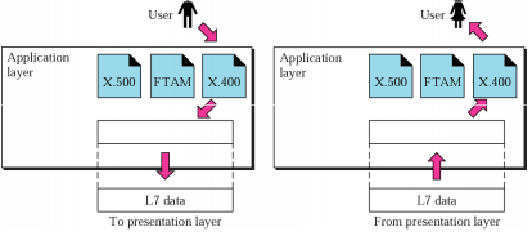
\includegraphics[width=8.92450478814115cm,height=3.94405089859635cm]{IIW-Reds-35.pdf}}
  \caption{}
\end{figure}}}

\paragraph{Internet Protocol Stack}

{\center{\begin{figure}[h]
  \raisebox{0.0\height}{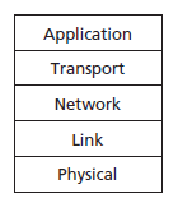
\includegraphics[width=2.97482946346583cm,height=3.39979338842975cm]{IIW-Reds-36.pdf}}
  \caption{}
\end{figure}}}
\begin{itemize}
  \item \tmtextbf{Applicazione:} il livello di applicazione {\`e} dove
  risiedono le appicazioni di rete e i loro protocolli di livello
  applicazione. Un suo esempio {\`e} il protocollo HTTP.
  
  \item \tmtextbf{Trasporto:} il livello di trasporto trasporta i messaggi del
  livello di applicazione e in Internet ci sono 2 protocolli principali
  \tmtextbf{UDP,TCP.}
  \begin{itemize}
    \item \tmtextbf{TCP:} fornisce un servizio a connessione, garantendo la
    consegna dei messaggi del livello applicativo. Inoltre, si divono i
    messaggi lunghi in segmenti pi{\`u} piccoli e fornisce un meccanismo di
    gestione della congestione.
    
    \item \tmtextbf{UDP:} fornisce un servizio non a connessione. Non si
    garantisce la consegna dei messaggi, nessun controllo di flusso e
    congestione.
  \end{itemize}
  \item \tmtextbf{Rete}: Il livello di rete {\`e} responsabili per spostare
  pacchetti del livello di rete, detti \tmtextbf{datagrammi}, da un host
  all'altro. Questo livello include il protocollo IP che definisce i campi nel
  datagramma permettendo di definire come i router e gli end-system si devono
  comportare.
  
  Inoltre si hanno anche protocolli di routing che determinano i percorsi che
  i datagrammi devono prendere fra sorgente e destinazione.
  
  \item \tmtextbf{Link:} Ad ogni nodo, il livello di rete passa il datagramma
  lungo il livelllo di link, il quale consegna il datagramma al prossimo nodo
  lungo il routing. Al prossimo nodo, il livello di linl passa il datagramma
  su il livello di rete. Il servizio dipende dallo specifico protocollo
  impiegato sul link. Quindi si ha il trasporto dei frame tra elementi di rete
  adiacenti.
  
  \item \tmtextbf{Physical:} la responsabilit{\`a} del livello fisico {\`e}
  quello di trasportare i singoli frame all'interno del frame da un nodo
  all'altro. I protocolli in questo livello sono dipendenti dal timpo di link
  e dal mezzo trasmissivo di esso.
\end{itemize}



{\center{\chapter{Application Layer}}}
{\center{\begin{figure}[h]
  \raisebox{0.0\height}{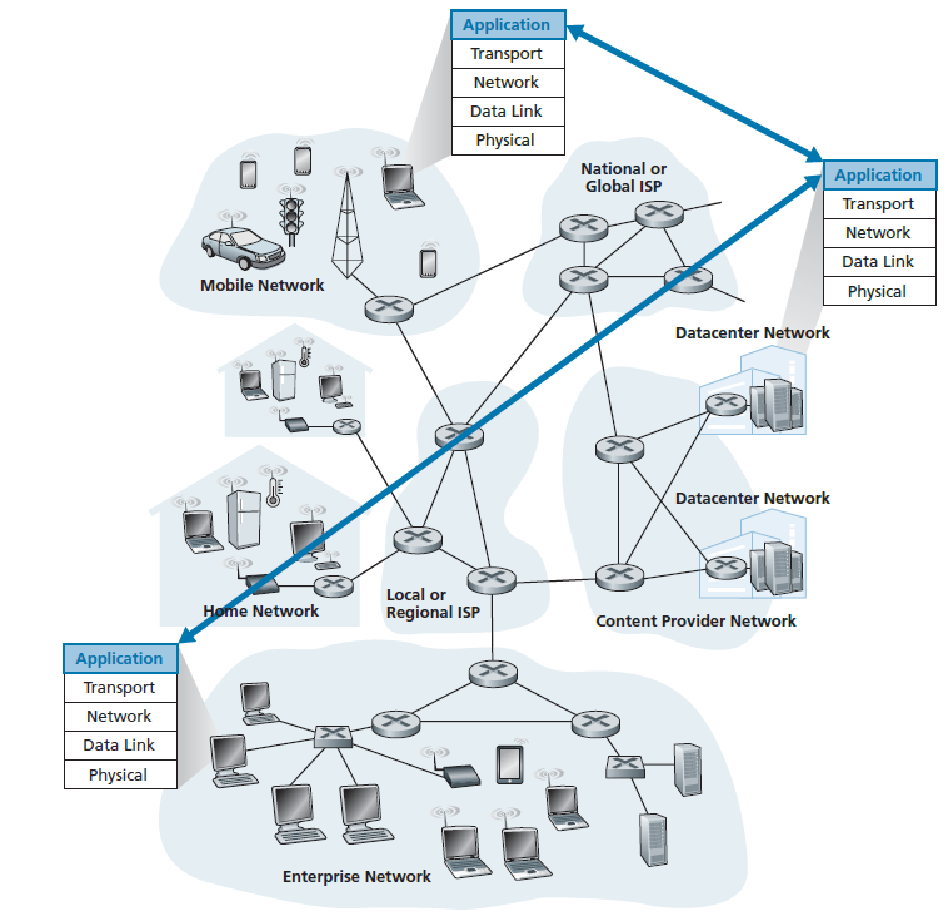
\includegraphics[width=15.915354847173cm,height=15.3829693034238cm]{IIW-Reds-37.pdf}}
  \caption{}
\end{figure}}}

\section{Architettura Applicazione di Rete}

L'\tmtextbf{architettura dell'applicazione}, {\`e} progettata dallo
sviluppatore dell'applicazione e regola come l'applicazione {\`e} strutturata
tra i vari end-system. Quindi lo sviluppatore dovr{\`a} decidere fra due
paradigmi architetturare: l'achitettura client-server o peer-to-peer (P2P):
\begin{itemize}
  \item nell'\tmtextbf{architettura client-server}, vi {\`e} sempre un host
  sempre acceso, detto \tmtextbf{server} che viene richiesto da molti altri
  host, detti \tmtextbf{client}. Inoltre, il server {\`e} ``fissato'',
  cio{\`e} possiede un indirizzo noto, detto \tmtextbf{indirizzo IP}
  poich{\'e} {\`e} sempre acceso e deve essere contantato da un qualsiasi
  host.
  
  In questo tipo di archittetura, un server non sempre riesce a gestire tutte
  le richieste dai client; a tale scopo si utilizzando i \tmtextbf{data
  center} che ospitano numerosi server con lo scopo di creare un potente
  server virtuale.
  
  \item nell'\tmtextbf{architetture P2P (peer-to-peer)} ci si affida in minima
  parte ai server dedicati e invece di avere una comunicazione con un server
  la si ha con un altro host. Gli host che intervengono in questa
  comunicazione vengono detti \tmtextbf{peers}. I peer non appartengono ad un
  provider del servizio, ma sono i desktop/laptop degli utenti. Questo tipo di
  architettura {\`e} molto \tmtextbf{scalabile}, cio{\`e} in caso di un numero
  elevato di utenti (peer) la capacit{\`a} di comunicazione aumenta. Tuttavia,
  non vi sono garanzie di sicurezza,performance e affidabilit{\`a}.
\end{itemize}

\section{Comunicazione tra processi}

Prima di costruire l'applicazione di rete, bisogna comprenre come i programmi,
in esecuzione su molteplici end-system, comunicano tra di loro. Nel dettaglio,
chi comunica non {\`e} il programma ma il \tmtextbf{processo} secondo le
regole dell'end-system. Quindi i processi su differenti end-system comunicano
tra di loro scambiandosi \tmtextbf{messaggi} attraverso la rete del computer.

\paragraph{Processi Client and Server}

Un'applicazione di rete consiste di una coppia di processi che si inviano
messaci tra di loro nella rete. Per ogni coppia di processi comunicanti, si
definisce un \tmtextbf{server} e un \tmtextbf{client} tramite la seguente
regola:
\begin{itemize}
  \item Il processo che inizia la comunicazione {\`e} detta \tmtextbf{client};
  
  \item Il processo che aspetta di essere contatato per iniziare la sessione
  {\`e} detto il \tmtextbf{server}.
\end{itemize}
Nel Web, i processi del browser (client) inizializzano il contato con i
processi del Web Server(server).

In un'architettura P2P, quando il peer A chiede al peer B di inviare uno
specifico file, il peer A {\`e} detto client mentre il peer B {\`e} il server.

\paragraph{Interfaccia fra i processi e la rede del computer}

Ogni messaggio inviato da un processo all'altro deve attraversare la rete. Un
processo invia e riceve un messagio attraverso un'interfaccia detta
\tmtextbf{socket}. In particolare, {\`e} l'interfaccia che risiede tra il
livello di applicazione e il livello di trasporto all'interno dell'host e
pu{\`o} esser detto anche \tmtextbf{Application Programming Interface (API)}
tra l'applicazione e la rete poich{\'e} il socket {\`e} l'interfaccia di
programmazione su cui si costruisce l'applicazione di rete.

Lo sviluppatore ha il controllo di tutto quello che accate dalla parte del
livello applicativo del socker (User Agent \tmtextbf{UA}), ma ne ha poco nella
parte del livello di trasporto del socket: tra cui la scelta del protocollo di
trasporto e forse la possibilit{\`a} di modificare la massima dimensione del
buffer e del segmento..

{\center{\begin{figure}[h]
  \raisebox{0.0\height}{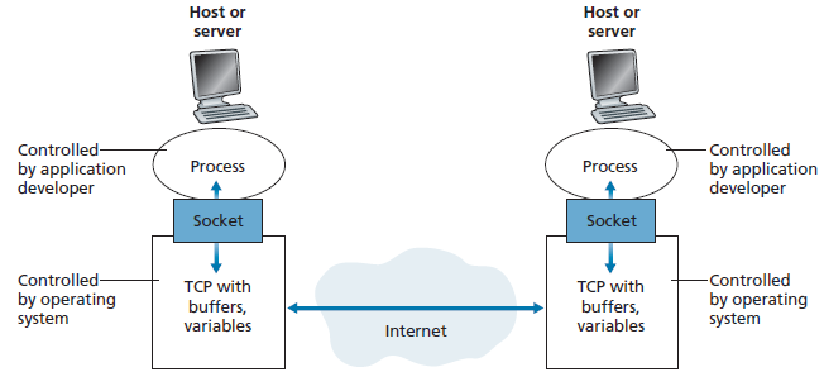
\includegraphics[width=13.8329725829726cm,height=6.22341925751017cm]{IIW-Reds-38.pdf}}
  \caption{}
\end{figure}}}

\subsubsection{Indirizzamento dei processi}

Affinch{\'e} il processo in esecuzione su un host invii i pacchetti al
processo in esecuzione su un'altro host, il processo ricevente deve avere un
indirizzo specificando:
\begin{itemize}
  \item l'indirizzo dell'host;
  
  \item identificatore che specifica il processo ricevente nell'host di
  destinazione.
\end{itemize}
In intetnete, l'host possiede il proprio \tmtextbf{indirizzo IP} composto da
32-bit. Inoltre, per conoscere l'indirizzo dell'host a cui {\`e} destinato il
messagge, il processo mittente deve identificare il processo ricevente
poich{\'e} un host potrebbe avere in esecuzione tante applicazioni di rete;
quindi si introduce il \tmtextbf{numero di porta} da 16 bit (0 non {\`e}
usati).

\subsubsection{Servizio di trasporto disponibile alle applicazioni}

L'applicazione invia i messaggi all'interno del socket, dall'altra parte il
protocollo del livello di trasporto, ha la responsabilit{\`a} di prendere il
messaggio dal socket. Moltre reti forniscono molti protocolli di trasporti di
rete tra cui scegliere in base ai servizi offerti dal protocollo:

\paragraph{Trasferimento affidabile di dati:}

Per supportare le applicazioni in cui le informazi sono fondamentali, bisogna
garantire che i dati inviati siano consegnati correttamente e completamente
dall'altra parte dell'applicazione. Se un protocollo fornisce un servizio di
cosnegna dati garantita, allora il dato inviato correttamente e interamente e
viene detto \tmtextbf{trasferimento affidabile di dati.}

Al contrario, se un'applicazione non fornisce questo servizio, allora si
potrebbero avere delle perdite al processo ricente. Questo tipo di
applicazioni vengono dette \tmtextbf{applicazioni loss-tolerant}. Ne sono un
esempio le applicazioni multimediali.

\paragraph{Throughput}

Poich{\'e} le altre sessioni condivideranno la bandwidth lungo il percorso di
rete, e poich{\'e} queste altre connessioni possono interrompersi, il
\tmtextbf{throughput} disponibile pu{\`o} fluttuare nel tempo.

Un servizio che pu{\`o} essere offerto {\`e} quello di \tmtextbf{garantire un
trhoughput} disponibile ad un certo rate. Da cui, un'applicazione potrebbe
richiedere un throughput di $r \frac{\tmop{bit}}{s}$, e il protocollo di
trasporto dovrebbe garantirne almeno quella quantit{\`a}.

Nel caso in cui il protocollo di trasporto non pu{\`o} fornire quel
throughput, l'applicazione dovrebbe codificare ad un rate minore o abbandonare
la connessione finch{\'e} non ha il rate necessario. Tali applicazioni vengono
detti \tmtextbf{bandiwidth-sensitive application}; altrimenti vengono datti
\tmtextbf{elastic application}.

\paragraph{Timing}

Un protocollo di livello di trasporto pu{\`o} fornire delle garanzie sul
tempo. Ne sono un esempio le applicazioni real-time in cui l'influenza del
tempo e dei ritardi assume una ruolo centrale.

\paragraph{Sicurezza}

Un protocollo di trasporto pu{\`o} fornire un'applicazione con uno o pi{\`u}
servizi di di sicurezza che, cifrando i dati prima della consegna , fornisce
una comunicazione confidenziale tra due processi anche se il messaggio pu{\`o}
essere osservato.

{\center{\begin{figure}[h]
  \raisebox{0.0\height}{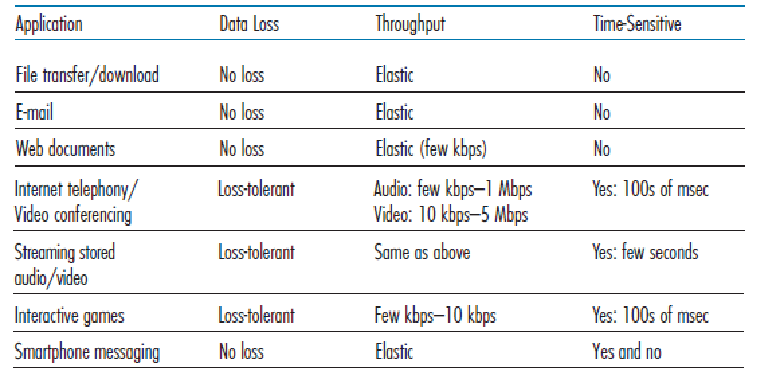
\includegraphics[width=13.089269316542cm,height=6.274432638069cm]{IIW-Reds-39.pdf}}
  \caption{}
\end{figure}}}

\subsubsection{Servizi di trasporto offerti da Internet}

Internet mette a disposizione delle applicazioni due \tmtextbf{protocolli di
trasporto:} UDP e TCP.

\paragraph{Servizi TCP}

Il modello del servizio TCP include un servizio di a connessione e un servizio
di trasferimento dati affidabile. Quando un'applicazione invoca TCP come suo
protocollo di trasporto, essa riceve entrambi i servizi:
\begin{itemize}
  \item {\underline{Connection-oriented service:}} TCP fa in modo che client e
  server si scambino informazioni di controllo a livello di trasporto prima
  che i messaggi di livello di applicazioni iniziano a fluire. Questa
  procedura {\`e} detta \tmtextbf{handshaking} preaparando il client e il
  server alla partenza dei pacchetti. Dopo questa fase, si dice che esiste una
  \tmtextbf{connessione TCP} tra le socket dei due processi. Viene detta anche
  connessione full-duplex poich{\'e} entrambi possono inviare dati. Quando
  l'applicazione termina l'invio deve chiudere la connessione;
  
  \item {\underline{Servizio di trasferimento affidabile:}} I processi
  comuniccanti pososno contare su TCP per trasportare dati senza errori e nel
  giusto ordine. Quando un lato dell'applicazione passa un flusso di byte alla
  sua socket, pu{\`o} affidarsi a TCP per consegnare lo steso flusso di byte
  alla socket di ricezione senza perdiata o duplicazione di byte;
  
  \item TCP include anche un meccanismo di controllo della congestione
  applicando una ``strozzatura'' del processo d'invio quando il traffico in
  rete appare eccessivo.
  
  \ 
\end{itemize}

\paragraph{Servizi di UDP}

UDP {\`e} un protocollo di trasporto leggere dotato di servizi minimalisti.
Infatti, {\`e} senza connessione, non necessita di hadshakinh e fornisce un
servizio di dati non affidabile.

Il protocollo, quindi. non garantisce che il messaggio raggiunga il processo
di destinazione ne che questi arrivino con lo stesso ordine in cui siano stati
inviati.

\subsection{Web e HTTP}

\subsubsection{Web}

Il \tmtextbf{Web} {\`e} una collezione di risorse/oggetti distribuiti
all'interno dei server della rete. Ogni oggetto/risorsa pu{\`o} essere un file
statico su una macchina o richieste generate dinamicamente. Il Web opera su
richiesta: si pu{\`o} avere ci{\`o} che si vuole, quando lo si vuole.

Una \tmtextbf{pagina web} {\`e} un contenitore di risorse come un file HTML
sul calo sono inclusi dei collegamenti a degli oggetti indirizzabile tramite
un \tmtextbf{URL}. L'indirizzamento avviene in questa manire:
{\center{https://www.blog.libero.it/wp/animelovers/2021/}}
\begin{itemize}
  \item \tmtextbf{Protocollo:} ``https'' che definisce coma la pagina viene
  acceduta;
  
  \item \tmtextbf{Nome dell'host:}''://www.blog.libero.it'' che indica dove la
  pagina {\`e} localizzata;
  
  \item \tmtextbf{Percorso del file:}\quad ''/wp/animelovers/2021/`` {\`e} il
  path alla risorsa di rete.
\end{itemize}

\subsection{Protocollo HTTP}

Un \tmtextbf{browser web} implemente il lato client di HTTP mentre un
\tmtextbf{web server} implementa il lato server di HTTP ospitando gli oggetti
web indirizzabili tramite URL.

HTTP definisce come i \tmtextbf{clients web} richiedono le \tmtextbf{pagine
web} ai \tmtextbf{web servers} e come i server trasferiscono le pagine web ai
clients.

{\center{\begin{figure}[h]
  \raisebox{0.0\height}{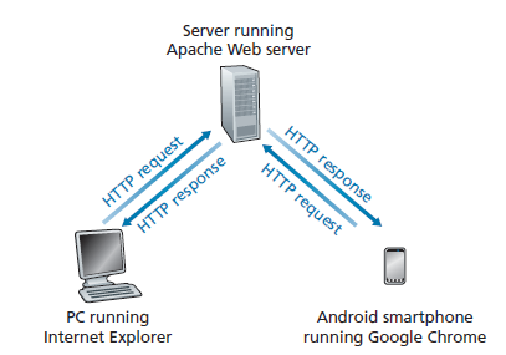
\includegraphics[width=8.49314574314574cm,height=5.95912042502952cm]{IIW-Reds-40.pdf}}
  \caption{}
\end{figure}}}

Quando un utente richiede la pagina Web, il browser invia al server messaggi
di richiesta HTTP per gli oggetti nella pagina. Il server ricevere la
richiesta e risponde con un nessaggi di risposta HTTP contenenti gli oggetti.

Il protocollo HTTP utilizza il protocollo TCP come il suo protocollo di
livello inferiore. Infatti, il client HTTP instaura una connessione TCP con il
server nella porta 80 e una volta che {\`e} stabilita, i processi del browser
e il server accedono a TCP attraverso le proprie socket.

Una volta che il client invia un messaggio nella sua interfacci socket,
quest'ultimo {\`e} in mano al protocollo TCP che garantisce un servizio
affidabile di trasferimento dati ad HTTP. Questo implica che ogni messaggio di
richiests HTTP inviato da un processo client arriva intatto al server e
viceversa; il protoccollo HTTP non si interessa su come vengono recuperati i
dati o su come vengono riordianti.

Inoltrem il servere invia i files richieste al client senza sapere nessuna
informazione sul client; ci{\`o} implica che se un client chiede in un periodo
di tempo ravvicinato lo stesso file, il server non risponde dicendo che
l'oggetto {\`e} gi{\`a} stato servito, ma risponde come se fosse stata la
prima connessione. Data questa propriet{\`a} ( di non mantenimento di
informazioni sul client), il protocollo HTTP {\`e} detto \tmtextbf{protocollo
stateless.}

\subsubsection{Connessione HTTP}

In molte applicazioni Internet, client e server comunicano per un lungo
periodo di tempo, con il client che inoltra una serie di richieste e il server
che risponde a ciascuna di esse. A seconda del tipo di interazione fra i due,
il progettista dell'applicazione deve scegliere quale tipo di connessione
adottare: \tmtextbf{connessioni HTTP persistenti, connessioni HTTP non
persistenti}.

\paragraph{Connessione HTTP non persistente}

Analizziamo nel dettaglio i passi di trrasferimento di una pagina Web dal
server al client nel caso di connessione non persistente:

{\center{\begin{figure}[h]
  \raisebox{0.0\height}{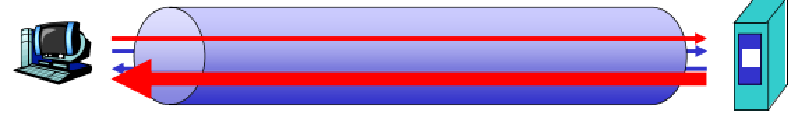
\includegraphics[width=13.3867407844681cm,height=1.99708120162666cm]{IIW-Reds-41.pdf}}
  \caption{Esempio grafico connessione non persistente HTTP}
\end{figure}}}
\begin{enumerate}
  \item Il processo client HTTP innizia una connessione TCP al server sulla
  porta 80 di default. Associata a questa connessione TCP, dopo che il server
  ha accettato la connessione, ci sar{\`a} un socket al client ed uno al
  server;
  
  \item Il client HTTP invia una richiesta HTTP al server tramite il suo
  socket, questa richiesta contiene l'oggetto che richiede;
  
  \item Il processo HTTP del server riceve la richieste di messaggio nella sua
  socket e restituisce l'oggetto dal suo archivio, la incapsulta in un
  messaggio di risposta HTTP e la invia al client dalla sua socket;
  
  \item Il processo del server HTTP chiude la connessione;
  
  \item Il client HTTP riceve il messaggio di risposta e la connession TCP
  termina. La risposta contiene il file HTML e nel caso in cui vi sono delle
  referenze ad altri oggetti le esamina;
  
  \item Per ogni referenza all'interno del file HTML ripete i passi 1-5.
\end{enumerate}
Quindi nella \tmtextbf{connesisone non persistente}, il client deve avviare
una connessione ogni qual volta deve richiedere un oggetto al server avviando
una connessione TCP,inviando una richiesta HTTP, aspettando la sua risposta e
nel caso ripetere.

In questa ottica, definiamo \tmtextbf{RTT- Round Trip-Time} il tempo
necessario affinche un piccolo pacchetto viaggi dal client al server e
viceversa. Questo parametro include:
\begin{itemize}
  \item ritardo di propagazione;
  
  \item ritardo di accodamento;
  
  \item ritardo di processamento;
  
  \item ritardo di trasmissione;
\end{itemize}
{\center{\begin{figure}[h]
  \raisebox{0.0\height}{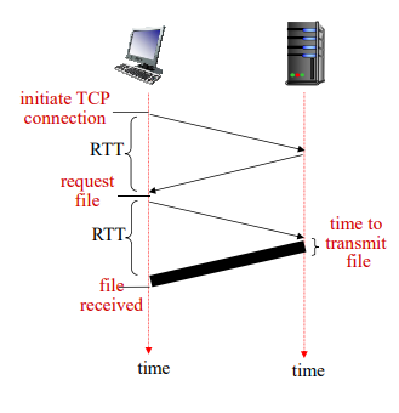
\includegraphics[width=6.69337859110586cm,height=6.93726223271678cm]{IIW-Reds-42.pdf}}
  \caption{}
\end{figure}}}

In totale quindi, avremo un ritardo del tipo:
\[ \tmop{Total} = 2 RTT + T_{\tmop{TX}} \]
Per ogni oggetto:
\[ \tmop{Total} = \sum_i^n (2 RTT + T_{\tmop{TX}}) \]

\paragraph{Difetti connessioni HTTP non persistenti}

I difetti di questo tipo di connessione sono i seguenti:
\begin{itemize}
  \item Per ogni oggetto richiesto occorre aspettare $2 RTT$;
  
  \item Si ha un consumo di risorse elevato;
  
  \item Anche considerando che un browser pu{\`o} avviare pi{\`u} connessioni
  in paralleli, esse gravano sul server che ne pu{\`o} gestire di meno.
\end{itemize}

\paragraph{Connessioni HTTP Persistenti}

Per le problematiche sopra riportate, una valida alternativa {\`e} quella di
ricorrere alle \tmtextbf{connessioni persistenti}.

{\center{\begin{figure}[h]
  \raisebox{0.0\height}{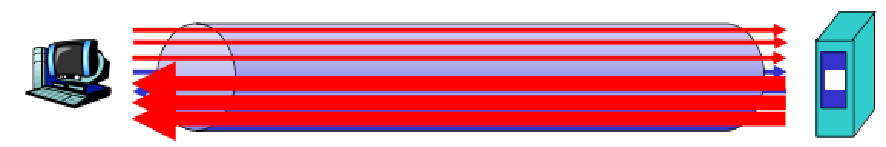
\includegraphics[width=14.8741637150728cm,height=2.4732880755608cm]{IIW-Reds-43.pdf}}
  \caption{}
\end{figure}}}

Nelle connessioni persistenti, il server lascia la connessione TCP aperto dopo
aver inviato la rispsota. Le successive richieste e risposte tra i due possono
essere inviati lungo la strssa connessione. Questo permette di inviare una
intera pagina Web su una singola persistente connessione TCP e, in alcuni
casi, inviare molteplici pagine Web contemporaneamente. Le connessioni
persistenti si differenziano in due tipologie:
\begin{itemize}
  \item \tmtextbf{Connessioni persistenti senza pipeling:} questi tipi di
  connessioni non consentono l'invio incontrollato di richieste e quindi di
  risposte tra client e server. In particolare, il client deve aspettare la
  risposta del server per effettuare la nuova richiesta mantenendo, per{\`o},
  la stessa connessione.
  
  Tramite questo tipo di connessione, l'RTT viene ridotto a 1 RTT ed in
  particolare, nel caso di invio di di richieste e risposte di n oggetti:
  \[ \tmop{Total} = RTT (1 + N) + \sum_{i = 1}^n T_{\tmop{TX}_i} \]
  \item \tmtextbf{Connessioni persistenti con pipeling:} questi tipi di
  connessionei consentono l'invio e la ricezione di richieste e risposte HTTP
  in contemporanea, senza quindi dover aspettare la risposta del server.
  Quindi il tempo che realmente viene speso {\`e} quello per
  l'inizializzazione della connessione TCP e per l'invio del primo oggetto. Il
  tempo totale per n oggetti vale:
  \[ \tmop{Total} = 3 RTT + \sum_i T_{\tmop{TX}_i} \]
\end{itemize}

\subsubsection{Messaggio di richiesta HTTP}

{\center{\begin{figure}[h]
  \raisebox{0.0\height}{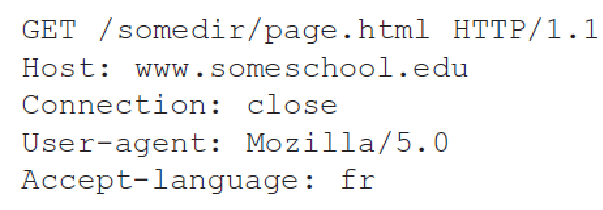
\includegraphics[width=10.1293126065853cm,height=3.53212317985045cm]{IIW-Reds-44.pdf}}
  \caption{Esempio di messaggio HTTP}
\end{figure}}}

I messaggi HTTP sono scritti in ASCII e facilmente comprensibili dall'uomo.
Esso consiste in 5 righe ognuna delle quali {\`e} seguita dal carattere di
ritorno e di nuova linea. L'ultima linea {\`e} seguita da un carattere di
ritorno e nuova linea aggiuntivo.

{\center{\begin{figure}[h]
  \raisebox{0.0\height}{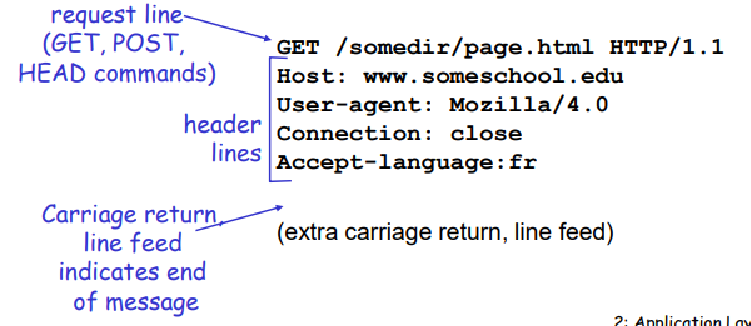
\includegraphics[width=12.6132920110193cm,height=5.48160173160173cm]{IIW-Reds-45.pdf}}
  \caption{}
\end{figure}}}
\begin{itemize}
  \item \tmtextbf{request line}: {\`e} la prima linea di un messaggio di
  richiesta HTTP. Essa {\`e} composta di tre campi:
  \begin{itemize}
    \item il campo del \tmtextbf{metodo}: pu{\`o} assumere diversi valori come
    GET,POST,HEAD,PUT e DELETE. Il metodo GET viene usato per richiedere un
    oggetto. Il metodo HEAD {\`e} molto simile al metodo GET, ma viene
    utilizzato in ambito di sviluppo poich{\'e} risponde alla richiesta HTTP,
    ma non invia l'oggetto richiesto. Il metodo PUT {\`e} utilizzato per
    caricare degli oggetti ai server Web e il metodo DELETE {\`e} utilizzato
    per eliminare un oggetto dal servewr Web;
    
    \item il campo \tmtextbf{URL} : condiente il percorso dell'oggett che deve
    essere gestito dal campo del metodo;
    
    \item il campo della \tmtextbf{versione} \tmtextbf{HTTP};
  \end{itemize}
  \item \tmtextbf{headerl line:} sono le linee che seguono la request line.
  Esso {\`e} composto da:
  \begin{itemize}
    \item \tmtextbf{Host:} specifica l'host su cui risiede l'oggetto. Viene
    specificato poich{\'e} necessario dalle caches Web;
    
    \item \tmtextbf{Connection:} il browser sta divendo che non vuole avere
    una connessione persistente e una volta in cui il server ha inviato
    l'oggetto richiesto, vuole che la connessione sia chiusa;
    
    \item \tmtextbf{User-Agent:} {\`e} il tipo di browser che sta facendo la
    richiesta. Questo {\`e} utile poich{\'e} i browser possono visualizzare le
    risorse in maniera differente;
    
    \item \tmtextbf{Accept-Language:} {\`e} una specifica su quale lingua
    vorrebbe ricevere la pagina HTML. Se non presente, viene inviata quella di
    default.
  \end{itemize}
  \item \tmtextbf{Entity body:} sono le line che seguono le blank line del
  messaggio di richiesta HTTP. Nel metodo get questo campo {\`e} vuoto; mentre
  nel metodo POST, molto utilizzato nella compilazione dei form, contiene i
  dati che si sono immessi all'interno del form.
\end{itemize}


{\center{\begin{figure}[h]
  \raisebox{0.0\height}{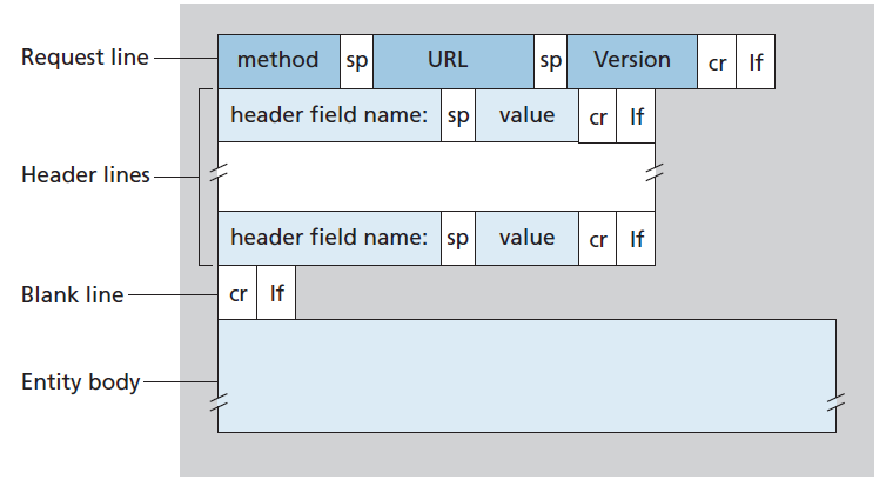
\includegraphics[width=14.8726715203988cm,height=8.16022235340417cm]{IIW-Reds-46.pdf}}
  \caption{Formato generale di un messaggio di richiesta HTTP}
\end{figure}}}

\subsubsection{Messaggio di risposta HTTP}

Il seguentne messaggio potrebbe essere il messaggio di risposta ad una
richiesta HTTP:

{\center{\begin{figure}[h]
  \raisebox{0.0\height}{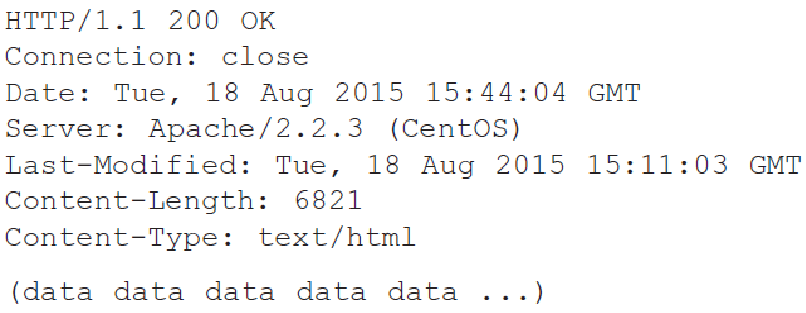
\includegraphics[width=13.5354847173029cm,height=5.26223271677817cm]{IIW-Reds-47.pdf}}
  \caption{}
\end{figure}}}

Il messaggio di risposta {\`e} formato da 3 sezioni: la \tmtextbf{riga di
stato},sei \tmtextbf{righe di intestazione} e il \tmtextbf{body}.
\begin{itemize}
  \item \tmtextbf{body}: contiene l'oggetto richiesto;
  
  \item \tmtextbf{status line:} {\`e} formato da 3 campi:
  \begin{itemize}
    \item il campo delle versione del protocollo;
    
    \item Il campo del codice di stato che indica il risultato della richiesta
    HTTP. I pi{\`u} comuni sono i seguenti:
    \begin{itemize}
      \item \tmtextbf{200 OK}: la richiesta {\`e} avvenuta con successo e
      l'informazioni {\`e} ritornata;
      
      \item \tmtextbf{301 Moved Permanently:} l'oggetto richiesto {\`e} stato
      spostato permanentemente e si specifica nel campo Location: il nuovo
      URL;
      
      \item \tmtextbf{400 Bad Request:} questo {\`e} il generico codice di
      errore che indica che la richiesta non {\`e} stata compresa dal server;
      
      \item \tmtextbf{404 Not Found:}Il documento richiesto non esiste su
      questo server;
      
      \item \tmtextbf{505 HTTP Version Not Supported:} La versione del
      protocollo di richiesta HTTP non {\`e} supportata dal server;
    \end{itemize}
    \item Il valore del codice di stato;
  \end{itemize}
  \item \tmtextbf{header line:} contiente:
  \begin{itemize}
    \item {\underline{Connection:}} indica che al client che sta per chiudere
    la connessione TCP una volta inviato il messaggio.
    
    \item {\underline{Date:}} indica la data e l'ora di quando la risposta
    HTTP {\`e} stata creata e mandata dal server. In particolare, coincide con
    il tempo in cui il server preleva l'oggetto dal proprio sisema, lo
    inserisce nel messaggio di rispsota e la invia.
    
    \item {\underline{Server}}: indica che il messaggio {\`e} stato generato
    da un certo server.
    
    \item {\underline{Last-Modified:}} indica la data e il giorno in cui
    l'oggetto {\`e} stato creato o modificato. Questa linea {\`e} utile per il
    chaching delle pagine Web nei proxy server.
    
    \item {\underline{Content-Lenght:}} indica il numero di bytes nell'oggetto
    che {\`e} stato inviato;
    
    \item {\underline{Content-Type:}} indica che il tipo dell'oggetto
    all'interno della risposta.
  \end{itemize}
\end{itemize}
{\center{\begin{figure}[h]
  \raisebox{0.0\height}{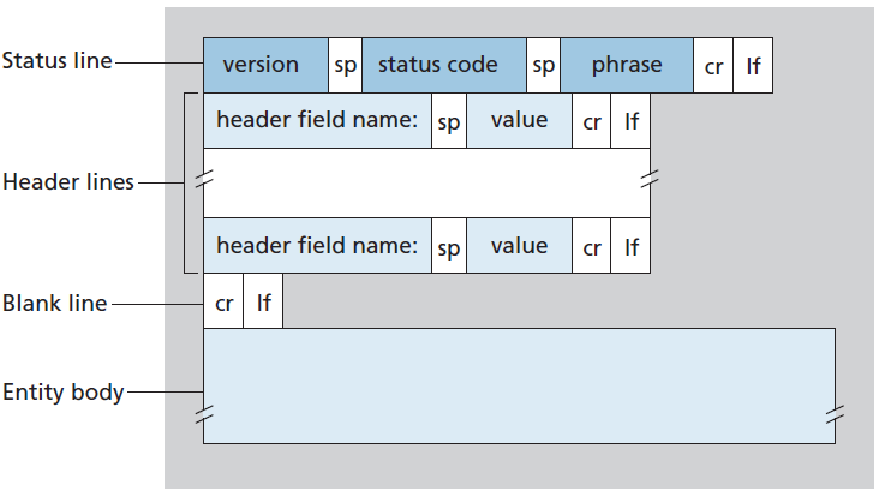
\includegraphics[width=14.8444182080546cm,height=8.32146136691591cm]{IIW-Reds-48.pdf}}
  \caption{}
\end{figure}}}

\subsubsection{User-Server Interaction: Cookies}

I server HTTP {\`e} stateless. Spesso il sito Web necessita di identificare
gli utenti, limitare le attivit{\`a} degli altri utenti o di personalizzare i
contenuti degli utenti. A tale scopo, si utilizzano \tmtextbf{cookies}.

I cookie sono formati da quattro componenti:
\begin{itemize}
  \item un riga di intestazione nel messaggio di risposta HTTP;
  
  \item una riga di intestazione nel messaggio di richiesta HTTP;
  
  \item un file mantenuta sul sistema dell'utente e gestito dal browser;
  
  \item un file mantenuto sul database sul sito.
\end{itemize}
{\center{\begin{figure}[h]
  \raisebox{0.0\height}{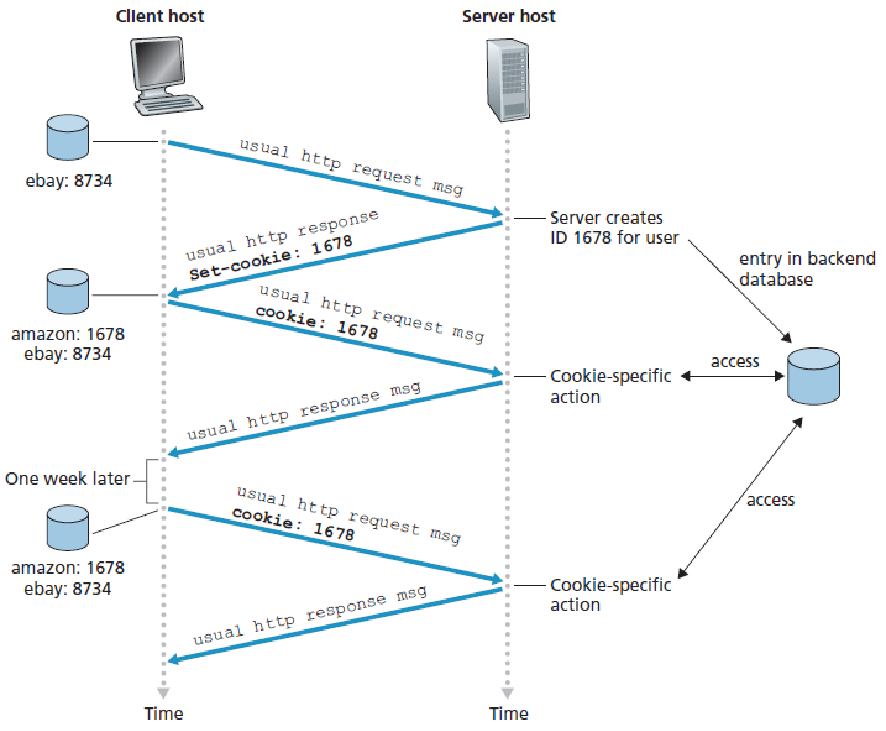
\includegraphics[width=14.8741637150728cm,height=12.2753181162272cm]{IIW-Reds-49.pdf}}
  \caption{}
\end{figure}}}

I cookies sono usati per identificare un utente. La prima volta in cui
l'utente visita il sito,l'utente fornisce un identificativo. Durante le
successive sessioni, browser trasferisce un cookie header al server per
permettere la sua identificazione nel server.

I cookie, inoltre, sono usati per creare una livello di sessione utente sul
protocollo HTTP stateless, inviando in ogni interazione le informazioni per
avere un'autenticazione automatica,

Riassumendo, i cookie permettono l'implementazione di un meccanismo di
autorizzazione, permettere di tenere traccia delle preferenze personali di
ogni utenti e quindi raccomandare/consigliare dei prodotti simili e permette
di tenere traccia dello stato della sessione utente. Tuttavia, vi {\`e} una
battaglia sull'eticit{\`a} di questi cookie al livello di privacy poich{\'e}
tramite essi si pu{\`o} conoscere molto sulle abitudini di un utente.

Per mantenere lo stato dell'utente, si necessitano di protocolli end point per
mantere lo stato del ricevente/mittente su molteplici transazioni e dei cookie
che portanto lo stato dei messaggi.

\subsubsection{Web Caching}

Una \tmtextbf{Web Cache} o \tmtextbf{proxy server} {\`e} un'entit{\`a} di rete
che soddista le richieste HTTTP al posto del Web server originario. Esso ha il
proprio dispositivo di archiviazione e mantiene le copie degli oggetti
recentemente richiesti.

Il browser di un'utente pu{\`o} essere configurato in modo tale che tutte le
richieste HTTP dell'utente vengano ridirette nella Web Cache.

Un proxy server funziona nella seguente maniera:
\begin{enumerate}
  \item Il browser stabilisce una connessione TCP al Web Cache e invia una
  richiesta HTTP per l'oggetto alla Web cache;
  
  \item La Web cache controlla se la copia dell'oggetto {\`e} salvata
  localmente. Se lo {\`e}, il proxy server ritorna l'oggetto all'interno di un
  messaggio di risposta HTTP al browser del client;
  
  \item Se il proxy server non possiede l'oggetto, la web chace apre una
  connessione TCP al server originario. A questo punto, il proxy server invia
  una richiesta di connessione TCP con il server originario ed invia la
  richiesta dell'oggetto;
  
  \item Quando la Web cache riceve l'oggetto, si salva una copia localmente e
  ne manda un'altra, all'interno di un messaggio di risposta HTTP, al browser
  del client.
\end{enumerate}
{\center{\begin{figure}[h]
  \raisebox{0.0\height}{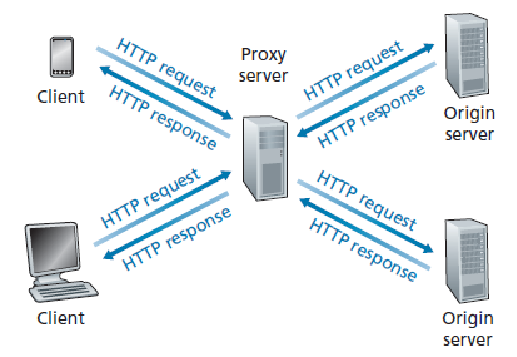
\includegraphics[width=8.68650793650794cm,height=5.99649088285452cm]{IIW-Reds-50.pdf}}
  \caption{}
\end{figure}}}

Come possiamo nota, la cache {\`e} sisa server che client durante l'intero
processo. Quando riceve la richiesta da e la invia ad un browser {\`e} un
server. Quando invia la richiesta a e la riceve la rispsota dal server di
orgine {\`e} un client.

La \tmtextbf{Web Caching} {\`e} utile per due motivazioni:
\begin{itemize}
  \item ricude il tempo di rispsota per una richiesta del client. In
  particolare, se il collo di bottiglia tra il client e il server di origine
  {\`e} molto minore rispetto il collo di bottiglia del client e della cache;
  se vi {\`e} un'altra velocit{\`a} di connessione tra client e cache, allora
  la cache riesce a rispondere alla richiesta molto velocemente;
  
  \item riduce il traffico di un'accesso istituzionale ad internet e quindi
  non si deve spendere per un miglioramento della rete.
  
  \item Riducendo globalmente il tempo di risposta, {\`e} possibile, quindi,
  migliorare il traffico sull'intero internet e migliore le prestazioni di
  tutte le applicazioni. 
\end{itemize}

\subsubsection{Get Condizionale}

Abbiamo introdotto il caching delle richieste HTTP dalla parte dei client al
fine di velocizzare l'intera rete fornendo una copia gi{\`a} salvata in un
browser o in proxy server. Tuttavia, questa copia potrebbe essere data sia a
causa di modifiche da parte del server; quindi HTTP possiede un meccanismo che
permette alla cache di verificare se un oggetto {\`e} datato. Questo
meccanismo {\`e} detto \tmtextbf{GET condizionale}.

Un messaggio di richiesta HTTP {\`e} detto di GET condizionale se presenta:
\begin{itemize}
  \item Il messaggo di richiesta utilizza il metodo GET;
  
  \item Il messaggio di richiesta include una riga di intestazione
  IF-Modified-Since
\end{itemize}
\begin{example}
  \
  
  Inizialmente, sotto richiesta di un browser, una proxy cache invia il
  messaggio di richiesta HTTP al Web server:
  
  {\center{\begin{figure}[h]
    \raisebox{0.0\height}{\includegraphics[width=6.77741702741703cm,height=0.990292535747081cm]{IIW-Reds-51.pdf}}
    \caption{}
  \end{figure}}}
  
  Successivamente il Web server invia un messaggio di risposta con l'oggetto
  richieste alla cache:
  
  {\center{\begin{figure}[h]
    \raisebox{0.0\height}{\includegraphics[width=8.32952905680178cm,height=2.70146267873541cm]{IIW-Reds-52.pdf}}
    \caption{}
  \end{figure}}}
  
  La cache inoltra l'oggetto alla browser, ma lo salva anche localmente.
  Inoltre, salva la data di ultima modifica.
  
  In seguito, un altro browser richiede lo stesso oggetto alla cache ed {\`e}
  ancora presento in esso. Dato che l'oggetot potrebbe essere modificato al
  Web Server nel tempo che intercorre tra le due richieste, la cache controlla
  se l'oggetto deve essere aggiornato istanziando un GET condizionale. In
  particolare:
  
  {\center{\begin{figure}[h]
    \raisebox{0.0\height}{\includegraphics[width=9.2814836678473cm,height=1.33005378459924cm]{IIW-Reds-53.pdf}}
    \caption{}
  \end{figure}}}
  
  La riga di intestazione IF-Modified-Since: equivale esattamente al valore
  della riga di intestazione Last-Modified del server della prima richiesta.
  Quindi, il GET condizionale sta dicendo al server di inviare l'oggetto se e
  solo se {\`e} stato modificato dalla data specificata.
  
  Supponiamo che l'oggetto non {\`e} stato modificato dalla data inviata dalla
  cache, allora il Web server invia un messaggio di risposta alla cache:
  
  {\center{\begin{figure}[h]
    \raisebox{0.0\height}{\includegraphics[width=7.13662600026236cm,height=2.10784796012069cm]{IIW-Reds-54.pdf}}
    \caption{}
  \end{figure}}}
\end{example}

Come si nota dall'esempio, il Web Server inviera comunque un messaggio di
risposta ma non include necessariamente l'oggetto richiesto dal messaggio
poich{\'e}, se l'oggetto non {\`e} stato modificato e fosse inviato comunque,
si sprecherebbe banda e si aumenterebbe il tempo di risposta percepito
dall'utente specialmente se l'oggetto in questione {\`e} di grande dimensione.

Riassumendo:

{\center{\begin{figure}[h]
  \raisebox{0.0\height}{\includegraphics[width=9.13273973501246cm,height=9.13273973501246cm]{IIW-Reds-55.pdf}}
  \caption{}
\end{figure}}}

\

\subsubsection{Trasferimento di file: FTP}

In una \tmtextbf{sessione FTP}, l'utente utilizza un host locale per
trasferire file da o verso un host remoto. Per accedere deve essere
autorizzato a scambiare tali informazioni con il file system remoto e quindi
deve fornire username e password. Dopo di che pu{\`o} trasferire file tra i
due file system.

{\center{\begin{figure}[h]
  \raisebox{0.0\height}{\includegraphics[width=12.6430375180375cm,height=4.10627377672832cm]{IIW-Reds-56.pdf}}
  \caption{}
\end{figure}}}

L'utente interagisce con FTP tramite un agente softwar detto \tmtextbf{FTP
User Agent} fornendo inizialmente il nome dell'host remoto, in modo che il
processo FTP client nell'host locale stabilisca una connessione TCP con il
processo FTP server nell'host reoto e fornisce nome identificativo e password,
inviate sulla connessione TCP come parte dei comandi FTP. Dopo di che,
ottenuta l'autorizzazione pu{\`o} inviare i file dal file system locale a
quello remoto.

\paragraph{HTTP e FTP a contronto}

HTTP e FTP sono protocolli di trasferimento di faile e condividono molte
caratteristiche in comune tra cui l'utilizzo della connessione TCP. Tuttavia,
FTP utilizza due connessioni TCP dette \tmtextbf{connessione di controllo} e
\tmtextbf{ connesione dati}
\begin{itemize}
  \item \tmtextbf{connessione di controllo:} viene utilizzata per inviare
  informazioni di controllo tra gli host come utente e password, per cambiare
  directory remote e comandi per inviare e ricevere file. La porta utilizzata
  {\`e} la prota 21;
  
  \item \tmtextbf{connesione dati:} {\`e} la connessione su cui si inviano e
  ricevono effettivamente i dati; la porta utilizzata {\`e} la porta 20.
\end{itemize}
Data la propriet{\`a} per cui FTP utilizza una connessione di controllo per i
dati viene detta \tmtextbf{fuori banda}; mentre il protocollo HTTP {\`e}
\tmtextbf{in banda} poich{\'e} utilizza una sola connessione per i dati e per
i dati di controllo.

In particolare quando un utente inizia una sessione FTP con un host remoto, il
lato client di FTP inizializza, come prima cosa, una connessione di controllo
TCP sulla porta 21 del lato server in cui invia l'identificativo e la
password.

Inoltre, si spedisce sulla connesisone di controllo i comandi per cambiare
directory remota. Quando il lato srrver riceve sulla connessione di controllo
un comando di trasferimento file inizializza una connessione dati TCP verso il
lato client sulla porta 20. Ftp invia essattamente un file sulla conessione
dati e poi la chiude. Se, durante la stessa sessione, l'utente volesse
trasferire un altro file, FTP aprirebbe un'altra connessione dati; pertanto la
connessione di contrllo rimane apreta per l'intera durata della sessione
utente, ma viene creata una di dati ogni qual volta si riceve il comando di
ricezione file.

Un'altra differenza con HTTP {\`e} che il protocollo FTP deve mantenere lo
\tmtextbf{stato} dell'utente. In particolare, associa la connessione di
controllo ad uno specifico utente e tiene traccia della directory corrente
dell'utente mentre quest'ultimo visita l'abero delle directory sull'host
remoto al fine di limitando, di conseguenza, il numero totale di sessioni che
FTP riesce a gestire contemporaneamente.

\subsubsection{Comani e risposte FTP}

I compandi dal client al server e le rispsota dal server al client sono
inviati attraverso la connessione di controllo in formato ASCII 7bit. Quinid,
i comandi FTP possono essere letti dall'utente come quelli di HTTP.

Inoltre, ogni comando consiste di 4 caratteri ASCII masiuscoli seguiti da un
argomento:
\begin{itemize}
  \item USER username:\quad utilizzato per inviar el'identificativo
  dell'utente al server;
  
  \item PASS password:\quad usato per inivare la password dell'utente al
  server;
  
  \item LIST:\quad utilizzato per chiedere al server di inviare un elenco di
  tutti i file nella directory remota corrente. Questa lista viene inviata
  attraverso la connessione dati;
  
  \item RETR filename:\quad usato per recuperare un file dall'attuale
  directory dell'host rempoto. Si forza l'host remoto ad inizializzare una
  connessione dati sulla porta 20 ed inviare il file;
  
  \item STOR filename:\quad Utilizzato per memorizzare un file nella directory
  corrente dell'host remoto.
\end{itemize}
Inoltre alcune risposte tipiche sono le seguenti:
\begin{itemize}
  \item 331 Username OK, password required:\quad il nome dell'utente {\`e}
  stato ricevuto, occorre inviare la password;
  
  \item 125 Data connection already open; transfer starting:\quad la
  connesisone dati {\`e} aperta, pu{\`o} iniziare il trasferimento;
  
  \item 425 Can't open data connection:\quad non {\`e} possibile aprire la
  connesione dati;
  
  \item 425 Error writing file:\quad si {\`e} verificato un errore nella
  scrittura del file.
\end{itemize}

\section{Posta elettronica}

Il servizio di posta elettronica {\`e} formato da 3 componenti:
\begin{itemize}
  \item \tmtextbf{User Agent}: permettono all'utente di leggere,rispondere,
  inoltrare,salvare e comporre i messaggi. Ne {\`e} un esempio Gmail.;
  
  \item \tmtextbf{Mail Servers}: rappresentano il nucleo dell'infrastruttura
  delle mail ed in ognuna di queste, per ogni utente vie {\`e} una
  \tmtextbf{mailbox} con il compito di manetere e gestire i messaggi che gli
  arrivano. Inoltre il loro compito {\`e} quello di gestire le code dei
  messaggi formatasi quando il tentativo di invio dei messaggi non {\`e}
  andato a buon fine;
  
  \item \tmtextbf{Simple Mail Transger Protocol-SMTP}: {\`e} un protocollo
  client/server in cui gli utenti non interagiscono tra di loro ma con il
  server di posta elettronica comunicando tra i messaggi trai di loro tramite
  i Mail Server. 
\end{itemize}
{\center{\begin{figure}[h]
  \raisebox{0.0\height}{\includegraphics[width=13.5354847173029cm,height=11.255821199003cm]{IIW-Reds-57.pdf}}
  \caption{}
\end{figure}}}

\paragraph{SMTP}

Il protocollo \tmtextbf{SMTP} {\`e} il principale protocollo di livello
applicativo per le email di Internet. Questo protocollo utilizza un servizione
di trasferimento dati di TCP per inviare dal server le email del mittente alla
\tmtextbf{mailbox} del destinatario. La porta utilizzata {\`e} la porta 25 ed
i messaggi che si inviano sono in 7-bit ASCII.

Inoltre, {\`e} formato da:
\begin{itemize}
  \item \tmtextbf{lato client:} eseguito dal mail server del mittente;
  
  \item \tmtextbf{lato server:} eseguito sulla mailbox del server.
\end{itemize}
Entrambi di questi lati sono in esecuzione sul server: quando il mail server
invia email ad un altro mail server si comporta da client, altirmenti da
server. In particolare si alternano 3 fasi:
\begin{itemize}
  \item handshaking;
  
  \item trasferimento di messaggi;
  
  \item chiusura della connessione.
\end{itemize}
\begin{example}
  {\tmdummy}
  
  \begin{enumerate}
    \item Alice invoca il suo User Agent per le e-mail fornendo l'indirizzo
    email di Bob, compone il messaggio e dice all'user agent di inviare il
    messaggio;
    
    \item L'user agent di Alice invia il messaggio al suo email server, dove
    sar{\`a} messo nella coda di messaggi;
    
    \item Il lato client di SMTP, in esecuzione sul server di Alice, vede il
    messaggio nella coda messaggi. Apre una connessione TCP sul server SMTP,
    in esecuzione sul mail server di Bob.
    
    \item Dopo un certo tempo di handshaking, il lato client di SMTP di Alice
    invia il messaggio sulla connessione TCP;
    
    \item Al mail server di Bob, il lato server di SMTP di Bob riceve il
    messaggio. Il mail server di Bob la posizione nella mailbox di Bob;
    
    \item Bob invoca il suo user agent e legge il messaggio quando vuole.
  \end{enumerate}
\end{example}

{\center{\begin{figure}[h]
  \raisebox{0.0\height}{\includegraphics[width=14.8741637150728cm,height=5.41125541125541cm]{IIW-Reds-58.pdf}}
  \caption{}
\end{figure}}}

\begin{remark}
  \
  
  Il protocollo SMTP non utilizza server intermediari tra i due utenti anche
  se questi si trovano a grandissima distanza.
\end{remark}

Nel caso in cui il server {\`e} down, il lato client SMTP prova l'invio del
messaggio inseguito. Una volta che la connessione {\`e} stabilita, il server e
il client attuano l'handshaking trasferendosi informazioni tra cui l'indirizzo
email del mittente e del destinatario. Dopo questa fase, si invia il
messaggio.

Inoltre, il protocollo SMTP si basa sul servizio di trasferimento dati
affidabile di TCP per inviare il messaggio al server senza errore.
Riapplicando questo procedimento per ogni messaggio da inviare al server, in
alternativa si chiude la connessione.

Dal lato client(C) e server(S) del protocollo SMTP, (C) indica le line che il
client invia alla sua TCP socket (S) quelle che il server invia alla sua TCP
socker:
\begin{itemize}
  \item (C) pu{\`o} inviare 5 comandi HELO,MAIL FORM, RCTP TO, DATA, QUIT;
  
  \item (S) risponde ad ogni comando con un codice di risposta ed
  opzionalmente delle frasi in inglese.
\end{itemize}
\begin{note}
  \
  
  Per ogni messaggio, il client inizia il processo con un MAIL FROM e finisce
  con QUIT solo dopo che tutti i messaggi sono stati inviati.
\end{note}

\subsection{Confronto SMTP e HTTP}

Entrambi i protocolli sono usati per trasferire i file da un host all'altro.
\tmtextbf{HTTP} trasferisce i file da un Web Server ad un Web client; mentre
\tmtextbf{SMTP} trasferisce file da un mail server ad un altro.

Quando si trsferiscono i file entrambi i protocolli utilizzano connessioni
persistenti.

Inoltre, HTTP {\`e} un \tmtextbf{protocollo pull} poich{\'e} qualcuno carica
informazioni su un Web server e gli utenti utilizzano HTTP per prelevare le
informazioni del server quando vogliono: la connessione TCP {\`e}
inizializzata dalla macchina che vuole ricevere il file; mentre il protocollo
SMTP, {\`e} un \tmtextbf{protocollo push}: il mail server mittente esegue un
``push'' del file al mail server ricevente. La connessione TCP {\`e} iniziata
dalla macchina che vuole inviare il file.

Il protocollo SMTP richiede che le mail siano scritte in carattere a 7-bit
ASCII mentre HTTP no. In conclusione, HTTP incapsula ogni oggetto in un
messaggio di risposta HTTP; SMTP, al contrario, tutti gli oggetti vengono
messi in un messaggio.

\subsection{Formato messaggi mail}

Quando un messaggio e-mail {\`e} inviato da una persona all'altra, vi {\`e} un
\tmtextbf{header} che contiente le informazioni che precedono, separato da una
linea vuota, il \tmtextbf{body} del messaggio stesso.

In particolare, contiente una serie di linee di intestazioni contententi:
\begin{itemize}
  \item From: chi {\`e} l'utente che invia la e-mail;
  
  \item To: a chi {\`e} indirizzata l'e-mail;
  
  \item Subject: cio{\`e} la specifica del contenuto dell'e-mail;
  
  \item \tmtextbf{MIME}: consente di specificare il formato del messaggio
  cos{\`i} da includere, talvolta, anche allegati multimediali (codificati
  all'interno del body). In caso di oggetti di vario tipo si utilizza la
  specifcia \tmtextbf{multi part type}.
\end{itemize}

\subsection{Mail Access Protocoll}

{\center{\begin{figure}[h]
  \raisebox{0.0\height}{\includegraphics[width=14.8741637150728cm,height=3.09996064541519cm]{IIW-Reds-59.pdf}}
  \caption{}
\end{figure}}}

Consideriamo ora il percorso che prende un'e-mail quando viene inviata ad un
User Agente. In un qualche punto lungo il percorso, l'email deve essere
depositata.Il protocollo SMTP {\`e} l'incaricato a questo compito. Infatti,
come gi{\`a} discusso, ha il compito di fare il push delle e-mail tra mail
servers mittente e destinatario.

In particolare, l'User Agent mittante utilizza SMTP per inviare il messaggio
nel proprio mail server ed {\`e} il mail server che utilizza nuovamente SMTP,
come client, per consegnare l'email all'User Agent destinatario.

\begin{note}
  Se avessimo pensato di inviare l'email direttamente tra due User Agents, non
  avremmo avuto la garanzia che il messaggio arrivi ed inoltre, avendo due
  mail server, uno in cui il mittente pusha il messaggio consente al mail
  server mittente di inviare ripetutametne la e-mail in caso di errori,
  finch{\'e} la consegna non {\`e} avvenuta con successo.
\end{note}

L'User Agent destinatario non pu{\`o} utilizzare il protocollo SMTP per
ottenre il messaggio poich{\'e} questa operazione {\`e} un'operazione pull,
quando il protocollo {\`e} push. A tale scopo si introducono tre protocollo di
accesso alle email: \tmtextbf{POP3,Access Protocol (IMAP)} e \tmtextbf{HTTP.}

\paragraph{POP3 - Post Office Protocol}

Il \tmtextbf{protocollo POP3} {\`e} un protocollo molto semplice, ma dalle
funzionalit{\`a} limitate. Inizia quando l'User agente apre una connessione al
mail server sulla porta 110. Quando la connessione TCP viene stabilita, POP3
segue 3 fasi:
\begin{itemize}
  \item \tmtextbf{Autorizzazione}: l'user agent invia, in chiaro, username e
  password per essere autenticato. I comandoi utilizzati sono:
  \begin{itemize}
    \item user <username>;
    
    \item pass <password>;
  \end{itemize}
  Una volta autenticato si passa alla prossima fase;
  
  \item \tmtextbf{Transazione:} l'user agent preleva i messaggi, pu{\`o}
  selezionare i messaggi da eliminare e ottenere le statistiche di email; ad
  ognuno di questi comandi il server risponde con due possibili opzioni:
  \begin{itemize}
    \item +OK: usato dal server per indicare che il precedente comando {\`e}
    andato a buon fine;
    
    \item -ERR: usato dal server per indicare che qualcosa {\`e} andato storto
    con il precedente comando
  \end{itemize}
  Inoltre, questa fase pu{\`o} essere configuarata per \tmtextbf{download and
  delete} o \tmtextbf{download and keep}. La sequenza dei comandi istanziati
  dall'user agente dipende su quali modi si sta operandi:
  \begin{itemize}
    \item download and delete mode: l'user agent utilizzer{\`a} i comandi
    list,retr,delete,quit. Dal lato del mail server, una volta ricevuto il
    comando quit eliminer{\`a} tutti i messaggi.
    
    \item download and keep: l'user agente utilizzer{\`a}\quad i comandi
    precedenti ad eccezzione del delet. I messaggi rimarranno salvati.
  \end{itemize}
  \item \tmtextbf{Update:} Il mail server elimina i messaggi segnati per la
  cancellazione;
\end{itemize}
Questo protocollo non mantiente informazioni sullo stato dell'user agent.

\paragraph{IMAP}

\tmtextbf{IMAP} {\`e} un protocollo di accesos mail, possiede pi{\`u}
funzionalit{\`a} di POP3, ma molto pi{\`u} complesso.

Un server IMAP associa ad ogni messaggio una cartella, quando un messaggio
arriva al server viene associato nella cartella INBOX. Talvola, la mailbox
pu{\`o} sportare l'e-mail in una cartella creata dall'utente, leggerla,
eliminarla.

Il protocollo IMAP fornisce dei comandi che permettono all'utente di creare
cartelle e muovere i messaggi tra le cartelle, di cercare messaggi che
corrispondono ad uno specifico criterio ed, inoltre, si mantengono
informazioni sullo stato dell'utente lungo la sessione.

\paragraph{HTTP}

Quando un utente vuole accedere alla propria mailbox, i messaggi vengono
spediti dal mail server al proprio browser utilizzando il protocollo HTTP.

Se volessimo inviare un messaggio, quest'ultimo {\`e} inviato dal browser al
mail server, dopo di che si utilizza il protocollo SMTP come visto fino ad
ora.

\section{DNS - Domain Name System}

Il \tmtextbf{DNS} nasce dall'esigenza di identificare gli host internet. Un
identificatore per un host, pi{\`u} conosciuto, {\`e} l'\tmtextbf{hostname}
(per esempio www.facebook.com), generalmente alfanumerico e forniscono
informazioni circa la posizione dell'host in internet. Poich{\'e} gli hostname
essendo alfanumerici e di lunghezza variabile non si prestano al routing che
deve fare un router per indirizzare hosts.

A tale scopo introduciamo gli \tmtextbf{indirizzi IP}. Essi sono indirizzi
gerarchici, poich{\'e} ogni periodo che va da 0 a 255 fornisce informazioni
aggiuntive sulla locazione del host, formati da 32 bit.

\subsection{Servizi forniti dal DNS}

Per avere un mapping tra \tmtextbf{hostname} ed \tmtextbf{indirizzo ip},
occorre un servizio di directory che traduce gli hostname in indiriziz IP. La
soluzione a questo problema {\`e} data dal \tmtextbf{domani name system DNS}.

Il DNS {\`e} un database distribuito, che utilizza il protocllo UDP alla porta
23, in una gerarchia di \tmtextbf{DNS servers} e un protocollo di livello
applicativo che permette agli host di eseguire query al database distribuito.
La traduzione viene effettuaata nel seguente modo:
\begin{itemize}
  \item L'utente esegue il lato client dell'applicazione DNS;
  
  \item Il borwser estrare l'hostname dall'URL e lo passa alla parte cliente
  dell'applicazione DNS;
  
  \item Il client DNS invia una query contentente l'hostname al DNS server;
  
  \item Il DNS client riceve una risposto che include l'indirizzo IP per
  l'hostname;
  
  \item Una volta che il browser ricere l'indirizzo IP dal DN, pu{\`o}
  iniziare una connessione TCP al processo server HTTP localizzato sulla porta
  80 dell'indirizzo IP.
\end{itemize}
Il protocollo DNS fornisce i seguenti servizi:
\begin{itemize}
  \item \tmtextbf{Host aliasing:} un host con un nome complicato pu{\`o} avere
  uno o pi{\`u} nomi che riferiscono allo stesso indirizzo IP;
  
  \item \tmtextbf{Mail server aliasing:} Il protocollo DNS pu{\`o} essere
  invocato da un'applicazione mail per ottenere dall'hostname l'indirizzo IP;
  
  \item \tmtextbf{Load distribution:} DNS {\`e} utilizzato anche per
  implementare una distribuzione di carico lungo i server replicati. I siti
  occupati vengono replicati su molteplici server, con ogni server in
  esecuzione su un diverso end system con un diverso indirizzo IP. Quindi a
  questi indirizzi IP si associa lo stesso hostname.
\end{itemize}
Un'implementazione effettiva di DNS potrebbe essere quella di centralizzare
tutte le traduzione degli indirizzi su un unico DNS server. Tuttavia, ci{\`o}
{\`e} irrelizzabile. Infatti, le problematiche sono le seguenti:
\begin{itemize}
  \item \tmtextbf{Single point failure:} Se l'unico server DNS va in crash, lo
  fa anche tutto Internet;
  
  \item \tmtextbf{Traffic Volume:} Un unico server DNS dovrebbe gestire tutte
  le query, per tutte le richieste HTTP, per i messaggi etc..
  
  \item \tmtextbf{Distant centralizer database:} Un singolo server DNS non
  pu{\`o} essere vicino a tutti i client che inviano query DNS;
  
  \item \tmtextbf{Manutenzione:} L'unico server DNS dovrebbe tenere traccia di
  tutti i record di tutti gli host internet. Oltre ad essere di grandi
  dimensioni, dovrebbe aggiornare frequentemente ogni host.
\end{itemize}
La soluzione a cui si {\`e} arrivati, {\`e} la realizzazione di un
\tmtextbf{database distribuito gerarchicamente}.

\

\paragraph{Database distribuito gerarchicamente}

\

Al fine di gestire il problema di \tmtextbf{scalabilit{\`a}}, il DNS utilizza
un grande numero di server (nessuno dei quali possiade la mappa di tutti gli
indirizzi IP), organizzati in maniera gerarchica distribuiti lungo tutto il
mondo. Vi sono tre classi di indirizzi server:
\begin{itemize}
  \item \tmtextbf{root DNS server:} forniscono l'indirizzo IP per i server
  TLD;
  
  \item \tmtextbf{top-level-domani DNS (TLD):} sono del tipo .com/.uk e
  forniscono l'indirizzo IP ai server autorirari;
  
  \item \tmtextbf{authoritative DNS server:} sono utilizzati per gli enti
  pubblici.
  
  \item \tmtextbf{local DNS server:} non fanno parte neccassariamente delle
  gerarchia, ma sono forniti dagli ISP che possono salvarsi gli hostname per
  velocizzare il loro servizio.
\end{itemize}
{\center{\begin{figure}[h]
  \raisebox{0.0\height}{\includegraphics[width=12.7769086973632cm,height=5.0274334251607cm]{IIW-Reds-60.pdf}}
  \caption{}
\end{figure}}}

\

\begin{example}
  {\underline{Query di DNS Locale}}
  
  Supponiamo che l'host desidera l'indirizzo IP di una pagina a tale scopo
  contata il suo DNS locale, che contatta il root server se necessario che
  contatta il server DNS autoritario se necessario ed infinite ritorna
  l'indirizzo IP all'host richiedente.
  
  {\center{\begin{figure}[h]
    \raisebox{0.0\height}{\includegraphics[width=8.49314574314574cm,height=10.5179883248065cm]{IIW-Reds-61.pdf}}
    \caption{}
  \end{figure}}}
  
  \begin{note}
    Utilizzando il caching il traffico viene molto diminuito.
  \end{note}
\end{example}

Come abbiamo visto nell'esempio, in generale, non potremmo conoscere il nome
del server autoritario, ma possiamo conoscere il server invermediario che deve
poter risalire al nome del server autoritario. A tale scopo pu{\`o} effettuare
due tipologie di query:
\begin{itemize}
  \item \tmtextbf{query ricorsive:} in cui si richiede la risoluzione del nome
  per suo conto. Potrebbe risultare tedioso per la rete;
  
  \item \tmtextbf{iterated query:} il server contattato risponde con un nome
  di un server da conttattare per risolvere il nome.
\end{itemize}
In altre parole, la query dall'host richiedente al server DNS {\`e} ricorsiva
e le rimanenti query sono iterative.

\

\paragraph{DNS Caching}

DNS sfrutta intensivamente il \tmtextbf{DNS caching} per migliorare le
performance sul ritardo e ridurre il numero di messaggi DNS in Internet.
L'idea {\`e} molto semplice: in una query a catena, quando un server DNS
risceve una risposta pu{\`o} mettere in cache locale il mapping tra hostname
ed indirizzo.

Se l'hostname/Indirizzo IP {\`e} in chace nel server DNS ed arriva un'altra
query per lo stesso hostname, il server DNS pu{\`o} fornire l'indirizzo IP
desiderato anche se non {\`e} autoritario.

Dal momento che gli hostname e gli indirizzi IP mediamente non sono
permanenti, i server DNS scartano le informazioni in cash dopo un certo
periodo di tempo.

\subsection{DNS Records and Messages}

\paragraph{DNS Records}

Il server DNS che implementano insieme il database DNS distribuito salvano
anche i \tmtextbf{record di risorsa RRs} che forniscono gli hostname
all'indirizzo IP. Ogni messaggio di risposta DNS porta uno o p{\`u} record di
risorsa. Esso {\`e} della seguente forma:

{\center{\begin{figure}[h]
  \raisebox{0.0\height}{\includegraphics[width=14.8741637150728cm,height=1.59158139839958cm]{IIW-Reds-62.pdf}}
  \caption{}
\end{figure}}}
\begin{itemize}
  \item \tmtextbf{TTL:} {\`e} il tempo di vita del record di risorsa.
  Determina quando la risorsa dovrebbe essere rimossa dalla cache;
  
  \item Il significato di \tmtextbf{Name }e \tmtextbf{Value} dipende dal
  \tmtextbf{Type}:
  \begin{itemize}
    \item Se \tmtextbf{Type=A}, allora \tmtextbf{Name} {\`e} l'hostname e
    \tmtextbf{Value} {\`e} l'indirizzo IP dell'hostname;
    
    \item Se \tmtextbf{Type=NS}, allora \tmtextbf{Name} {\`e} il dominio e
    \tmtextbf{Value} {\`e} l'hostname di un server autoritario che conosce
    come ottenere l'indirizzo IP per l'host di dominio;
    
    \item Se \tmtextbf{Type=CNAM}, allora \tmtextbf{Value} {\`e} l'hostname
    canonica per l'hostname alternativo \tmtextbf{Name}.
    
    \item Se \tmtextbf{Type=MX}, allora \tmtextbf{Value} {\`e} il nome
    canonico di un mail server che ha come alis hostname \tmtextbf{Name}.
  \end{itemize}
\end{itemize}
\begin{note}
  \
  
  Se un server DNS {\`e} autoritario per un particolare hostname, allora il
  server DNS conterra un record di tipo A per l'hostname;
  
  Se un server non {\`e} autoritario per l'hostname, allora il server
  contterra un record di tipo NS per il dominico che include l'hostname.
\end{note}

\paragraph{DNS Messages}

I messaggi di richiesta DNS possono essere di risposta o di query, aventi
entrambi lo stesso formato:

{\center{\begin{figure}[h]
  \tmtextbf{\raisebox{0.0\height}{\includegraphics[width=11.7803358257904cm,height=7.02835169880624cm]{IIW-Reds-63.pdf}}}
  \caption{Formato messaggio DNS}
\end{figure}}}
\begin{itemize}
  \item La prima \tmtextbf{sezione di intestazione} da 12 byte {\`e} formato
  da:
  \begin{itemize}
    \item Un campo per l'identificazione della query per permettere al client
    di confrontare le risposte ricevute con la query che ha inviato;
    
    \item Numerosi flag:
    \begin{itemize}
      \item flag di query/risposta: indica se il messaggio {\`e} una query o
      una risposta;
      
      \item flag autoritario: viene impostato in un messaggio di risposta
      quando un server DNS {\`e} un server atuoritario;
      
      \item flag di ricorsione: viene impostato quando un client desidera che
      il server DNS attui una ricorsione quando non si ha il record
      dell'hostname;
      
      \item flag di ricorsione disponible: viene impostato se il server DNS
      supporta la ricorsione;
    \end{itemize}
    \item Ulteriori quattro campi che indicano il numero di occorrenze dei
    quattro tipi di sezione di dati che seguento l'intestazione;
  \end{itemize}
  \item La \tmtextbf{sezione question} coniente informazioni sulle query che
  saranno effettuare. Include:
  \begin{itemize}
    \item un campo nome contenente il nome che viene richiesto;
    
    \item un campo tipo che indica il tipo di richiesta che si sta facendno;
  \end{itemize}
  \item La \tmtextbf{sezione di risposta} viene riempita in una rispsota da un
  server DNS. Contiente i recordi di risorsa per il nome che {\`e} stato
  originariamente chiesto, specificando Type,Value,TTL.
  
  \item La \tmtextbf{sezione autoritaria} contiene i record di altri server
  autoritari;
  
  \item La \tmtextbf{sezione addizionale} contiene altri record aggiuntivi.
\end{itemize}

\paragraph{Insert Records into the DNS Database}

La prima cosa che occorre fare quando si crea una compagnia {\`e} quello di
registrare il dominio al \tmtextbf{registar}. Essa {\`e} un'entit{\`a}
commerciale che verifica l'unicit{\`a} del nome del dominio, inserisce il nome
del dominio nel database DNS e chiede una tassa per questo servizio.

Inoltre, occorre fornire al \tmtextbf{registar} il nome e gli indirizzi IP dei
server DNS autoritari primari e secondari. A quel punto questa entit{\`a}
commergia si assicura che i record di {\underline{Type NS}} e {\underline{Type
A}} siano inseriti nel server Top-Level-Domain TDL; d'altra parte, la
compagnia deve accertarsi che i recordi di risorsa di Type A del Web Server e
di Type MX del mail server siano inseriti nel server DSN autoritario.

\section{Peer-to-Peer (P2P) File Distribution}

In una \tmtextbf{architettura P2P}, non vi {\`e} garanzia di presenza di
server sempre accesi. Al contrario, si hanno coppie intermittenti di host
connessi, detti \tmtextbf{peer}, che comunicano direttamente tra di loro.

Supponiamo di avere un applicazione P2P che permette la distribuzione di file
di granfi fimensioni da un singolo server a molteplici server. Quindi, ogni
peer pu{\`o} ridistribuire qualisiasi porzione del file che ha ricevuto su
qualsiasi altro peer. Cos{\`i} facendo, si supporta il compito del server di
distribuire questo file.

\paragraph{Scalablit{\`a} di un'architettura P2P}

Per confrontare un'architettura client-server con una peer-to-peer,
consideriamo un modello di distribuziine di un file con un numero fissato di
peer per entrambe le architetture.
{\center{\begin{figure}[h]
  \raisebox{0.0\height}{\includegraphics[width=9.95082316673226cm,height=8.5333202151384cm]{IIW-Reds-64.pdf}}
  \caption{}
\end{figure}}}
Il server e i peers sono connessi ad internet con i link. Definiamo:
\begin{itemizeminus}
  \item rate di upload del link di accesso del server $u_s$;
  
  \item rate di upload del link di accesso dell'$i$-esimo peer $u_i$;
  
  \item rate di download del link di accesso dell'$i$-esimo peer $d_i$;
  
  \item dimensione del file $F ;$
  
  \item il numero di peer che voglio ottenere la copia $N$;
\end{itemizeminus}
Il \tmtextbf{tempo di distribuzione} {\`e} il tempo speso per ottenere la
copia del file a tutti i peer.

Per entrambe le architettura, possiamo semplificare il modello assumendo che:
\begin{itemize}
  \item Il nucle di Internet possiede abbastanza bandwidth e tutti i colli di
  bottiglia si trovano nella reti di accesso;
  
  \item Il server e i client non partecipano in nessun'altra applicazione di
  rete. Quindi tutti i loro upload e download sono totalmente impiegati nel
  file.
\end{itemize}
Determiniamo il tempo di distribuzione per l'applicazione client-server
$D_{\tmop{cs}}$. In questo scenario, nessun peer contribuisce alla
distribuzione del file. In particolare:
\begin{itemize}
  \item Il server deve trasmettere una copia del file ad ogni peer.
  Trasmettendo cosi $N \ast F \tmop{bits}$. Dato che il rate di upload del
  server {\`e} $u_s$, impiegeremo $\frac{NF}{u_s}$ secondi;
  
  \item Definiamo $d_{\min}$ il rate di download del peer con il pi{\`u} basso
  rate di downlaod $d_{\min} = \{ d_{1,} d_2, \ldots, d_N \}$. Quest'ultimoi
  non pu{\`o} prendere il file in meno di $\frac{F}{d_{\min}}$ secondi.
\end{itemize}
Unendo queste cosiderazioni, possiamo scrivere il tempo di distribiuzione
come:
\[ D_{\tmop{cs}} \geqslant \max \left\{ \frac{NF}{u_s}, \frac{F}{d_{\min}}
   \right\} \]
Quindi il tempo cresce linearmente con il numero dei peers.

Invece, in una architettura P2P, ogni pper pu{\`o} contribuire nella
distribuzione del file. In particolare, quando un peer riceve qualche dato, lo
pu{\`o} usare con la propria capacit{\`a} di upload per ridistribuirlo ad
altri peer. Determiniamo il tempo di distribuzione del file:
\begin{itemize}
  \item All'inizio della distribuzione, solo il server possiede il file. Per
  prendere questo file nella community di peer, il server deve inviare ogni
  bit in almeno una volta nel suo access link. Inoltre il tempo di
  distribuzione minima {\`e} almeno $\frac{F}{u_s}$;
  
  \item Il peer con il minor download rate non pu{\`o} ottenere tutti gli $F$
  bit del vial in meno di $\frac{F}{d_{\min}}$ secondi. Il tempo di
  distribuzione {\`e} almento $\frac{F}{d_{\min}}$;
  
  \item La capcait{\`a} totale di upload del sistema per intero {\`e} uguale
  al rate di upload del server pi{\`u} i rate di upload di goni peer. Quindi,
  il sistema deve consegnare $F$ bit in ogni $N$ peer, consegnando in totale
  $NF$ ad un rate non maggiore di $u_{\tmop{tot}}$. Il tempo di distribuzione
  {\`e} almeno $\frac{NF}{(u_s + u_1 + \cdots + u_N)}$;
\end{itemize}
Unendo queste considerazioni, possiamo scrivere il tempo di distribuzione
come:
\[ D_{P 2 P} \geqslant \max \left\{ \frac{F}{u_s}, \frac{F}{d_{\min}},
   \frac{NF}{u_s + \sum^N_{i = 1} u_i} \right\} \]
{\center{\begin{figure}[h]
  \raisebox{0.0\height}{\includegraphics[width=10.5606552538371cm,height=6.71041584677948cm]{IIW-Reds-65.pdf}}
  \caption{}
\end{figure}}}

Ci{\`o} dimostra che all'aumentare del numero di untenti, il tempo di
distribuzione non cresce linearmente, provando la \tmtextbf{scalabilit{\`a}}
di un'architettura P2P conseguenza del fatto che i peer distribuiscono anche
il file.

\

\paragraph{BitTorrent}

BitTorrent {\`e} un'applicazione che utilizza il protocollo P2P. La collezione
di tutti i peer che partecipano nella distribuzione di un file {\`e} detto
\tmtextbf{torrent}. I peers in un torrent, scaricando i \tmtextbf{chunks}
della dimensione di 256KBytes di un file da un'altro peer.

Quando un peer si unisce ad un torrent, non possiede chunks, ma il accumula
durante il tempo. Mentre scarica i chunks, li mette a disposizione del torrent
e, una volta acquisito l'intero file, potrebbe lasciare il torrent o
contribuire all'upload del file.

\begin{note}
  \
  
  Si pu{\`o} lasciare e unire al torrent in qualsiasi momento.
\end{note}

{\center{\begin{figure}[h]
  \raisebox{0.0\height}{\includegraphics[width=13.3867407844681cm,height=9.25054112554113cm]{IIW-Reds-66.pdf}}
  \caption{}
\end{figure}}}

Ogni torrent possiede un nodo detto \tmtextbf{tracker}. Quando un peer si
unisce ad un torrent, si registra nel tracker ed informa periodicamente il
tracker che si trova ancora nel torrent.

Il tracker tiente traccia dei peer che partecipano al torrent.

Quando un nuovo peer, si unisce al torrent, il tracker selezione
randomicamente un sottoinsieme di peer da una lista di peer ed invia gli
indirizzi IP di questa lista. A questo punto il nuovo peer prova a stabilire
delle connessioni TCP concorrenti con tutti i peer, detti \tmtextbf{peer
vicini}, della lista che ha ricevuto. Con il passare del tempo, alcuni di
questi peer potrebbero lasciare il torrent ed altri provare a stabilire una
connessione TCP con il peer; facendo fluttuare la lista dei peer nel tempo.

Ad un dato istante, ogni peer avra un sottoinsieme di chunks del file e
periodicamente, si chiedera ad ogni peer vicino la lista dei chunk che
possiede. A questo punto per decidere quali chunk richiedere, si utilizza la
tecnica del \tmtextbf{il pi{\`u} raro prima.}

Al fine di velocizzare la distribuzione del file, si mandano i chunk pi{\`u}
rari prima.

Inoltre, occorre decidere a quali richieste i peer devono rispondere. A tale
scopo, BitTorrent utilizza un algoritmo di trading in cui si da priorit{\`a}
ai vicini che con cui stiamo scaricando al rate massimo. In particolare, per
ogni vicino, si misura continuamente il rate al quale ricevo i dati e si
determinano i 4 peer con il rate massimo. Ogni 10 secondi, si ricalola i rate
e il possibile insieme di 4 peer. Inoltre, ogni 30 secondi, si scegle un
vicino addizionale randomicamente e invia i chunk.

Se i due peer sono soddisfatti con lo scambio, si metteranno a vicenda nella
top quattro peers e continueranno a scambiarsi i chunk finch{\'e} saranno
compatibili.

\begin{note}
  \
  
  La selezione casuale del vicino permette ai nuovi peer di ottente chunk,
  cos{\`i} da avere la possibilit{\`a} di fare upload.
  
  Tutti i peer che sono al di fuori di questi cinque, non ricevono alcun
  chunk.
\end{note}

[Mancano Query flooding, Gnutella, e altre tipologie di P2P in disuso. Sul
libro non ci stavano, se presenti sugli esami, approfondire lezione 26 Marzo
2021]
{\center{\

\chapter{Transport Layer}}}

\section{Introduzione}

Tra il livello applicativo e di rete risiede il livello di transporto {\`e} il
nucleo dell'architettura di rete. Il \tmtextbf{livello di trasporto} ha la
responsabilit{\`a} di fornire servizi di communicazione direttamente ai
processi delle applciazioni in esecuzione sui differenti host.

Il problema principale di questo livello {\`e} capire come si effettua la
connessione affidabili su un mezzo che potrebbe perdere o corrompere i dati.
Inoltre, {\`e} importante capire come controllare il rate di trasmissione del
livello di trasporto per evitare, recuperare le congestioni all'interno della
rete.

\section{Servizi del livello di trasporto}

Il protocollo del livello di trasporto fornisce \tmtextbf{comunicazione
logica} tra i processi delle applicazioni sui differenti host. In particolare,
si intende che dalla prospettiva delle applicazione, {\`e} come se l'host
fosse connessio direttamente col procesos in esecuzione. L'applicazione
utilizza la comunicazione logica forna dal livello di trasporto per inviare i
messaggi tra di loro.

I protocollo del livello di trasporto, inoltre, sono implementati negli
end-system ma non nei routers di rete. Dalla parte del mittente, il livello di
trasporto converte i messaggi del livello applicativo che riceve dal processo
di un'applicazione del mittente in pacchetti di livello di trasporto, detti
\tmtextbf{segmenti}. Questo processo viene effettuato tramite la divisione dei
messaggi delle applicazioni in piccolo porzioni e, aggiungendo un'intestazione
ad ogni porzione, si crea il segmento del livello di trasporto.

A questo punto, il livello di trasporto invia il segmento al livello di rete
all'end-system del mittente, in cui il segmento viene incapsulato all'interno
di un pacchetto di livello di rete ed inviato a destinazione. Inoltre, {\`e}
importanto capire che i routers di rete si comportano solo sui campi del
livello di rete del datagramma e non esaminano i campi del livello di
trasporto.

Dal punto di vista del destinatario, il livello di rete estrae il segmento
del livello di trasporto dal datagramma e lo passa al livello di competenza. A
questo punto, il livello di trasporto riceve il segmento, lo rende disponibile
all'applicazione.

\section{Relazione tra livello di trasporto e di rete}

{\center{\begin{figure}[h]
  \raisebox{0.0\height}{\includegraphics[width=14.2792043814771cm,height=14.7245507018234cm]{IIW-Reds-67.pdf}}
  \caption{}
\end{figure}}}

Ricordiamo che il livello di trasporto giace appena sopra il livello di rete
nello stack di protocollo. Mentre un protocollo di livello di traspeto
fornisce communicazione logica tra i processi in esecuzione sui differenti
host. D'altra parte un protocollo di rete fornisce comunicazione logica tra
gli host.

\section{Protocolli di livello di trasporto in Internet}

Internet fornisce due \tmtextbf{protocolli di livello di trasporto} al livello
di applicazione.

Uno di questi protocolli {\`e} detto \tmtextbf{UDP} (User Datagram Protocol)
il quale fornisce un servizio inaffidabile, senza connessione alle
applicazioni che lo invocano. Il secondo protocollo {\`e} il protocollo
\tmtextbf{TCP}, il quale fornisce un\quad servizio affidabile, orientato alle
connessioni alle applicazioni invocanti.

Il protocollo di livello di rete {\`e} detto Internet Protocol \tmtextbf{IP};
esso {\`e} un \tmtextbf{servizio di consegna best-effort}. Questo significa
che IP rente il suo miglior sforzo per consegnare i segmenti tra host
comunicanti, ma non lo garantisce. In particolare, oltre a non garantire la
consegna dei messagi, non garantisce la consegna ordinata dei segmenti.

Per queste ragioni il servizio IP non {\`e} affidabile.

La responsabilit{\`a} fondamentale di UDP e TCP {\`e} quella di estendere il
servizio di consegna IP tra due end system a due processi in esecuzione sugli
end system. Questa estensione viene detta \tmtextbf{multiplexing e
demultiplexing.}

Inoltre, UDP e TCP fornisce un \tmtextbf{controllo di integrit{\`a}}
includendo campi di rilevamento errori nell'intestazione degli header. Questi
due servizi di livello di trasporto sono gli unici che il protocollo UDP
fornisce.

TCP, d'altro canto, offre servizi addizionali alle applicazioni. Prima di
tutto, fornisce un \tmtextbf{trasferimento di dati affidabile}. Utilizzano un
controllo di flusso, numeri di sequenza, ack e timer si assicura che i dadi
siano consegnati dal processo mittente al processo ricevente correttamente ed
in ordine.

Un'altra funzione di TCP {\`e} quello di convertire il servizio inaffidabile
di Internet Protocol tra gli enti syestm in uno affidabile tra processi e il
\tmtextbf{controllo di congestione} al fine di prevenire a qualsiasi
connession TCP di inondare i link e i router tra gli host comunicanti con
un'eccessiva quantit{\`a} di traffico.

\section{Multiplexing e Demultiplexing}

Le estensini offerte dal livello di trasporto sono il \tmtextbf{multiplexing}
e il \tmtextbf{demultipleaxing} che estendono il servizione di consegna
host-to-host fornito dal livello di rete in un servizio di consegna
process-to-process per le applicazioni in esecuzione sugli host.

In particolare, nell'host di destinazione, il livello di trasporto riceve i
segmenti dal livello di rete sottostante ed ha il compito di consegnare il
dato contenuto in questi segmenti al giusto processo d'applicazione in
esecuzione nell'host.

\begin{note}
  \
  
  Ricordiamo che un processo pu{\`o} avere uno o pi{\`u} \tmtextbf{socket}
  sul quale i dati passano dalla rete al processo e viceversa.
  
  Il livello di trasporto non trasporta il segmento direttamente al processo,
  ma al socket intermediario. Inotre, poich{\'e} in qualsiasi istante di tempo
  vi possono essere pi{\`u} di un socket nell'host ricevente, ogni socket ha
  un identificativo unico.
\end{note}

A questo punto quello che vogliamo capire {\`e} come un host ricevente
direziona un segmento alla giusta socket. A tale scopo, il segmento {\`e}
dotato di campi utili al compimento di questa funzione.

Il livello di trasporto controlla questi campi per identificare la socket
ricevente e la direzione su di essa. Questo processo viene detto
\tmtextbf{demultiplexing}.

Al contrario, il compito di raccogliere i \tmtextbf{chunk data} all'host
sorgente da diverse socket, l'incapsulamento di ogni chunk data con le
informazioni di instestazione per creare il segmento e il passaggio dei
segmenti nel livello di rete {\`e} detto \tmtextbf{multiplexing.}
{\center{\begin{figure}[h]
  \raisebox{0.0\height}{\includegraphics[width=14.5469303423849cm,height=7.19203397612489cm]{IIW-Reds-68.pdf}}
  \caption{}
\end{figure}}}
Il \tmtextbf{livello di trasporto}, per effettuare la
\tmtextbf{multiplazione}, richiede:
\begin{itemize}
  \item Socket con un identificativo univoco, detto \tmtextbf{source port
  number field};
  
  \item Ogni segmento deve posserede dei campi speciali che indicano la socket
  al quale il segmento deve essere consegnato, detto \tmtextbf{destination
  port number field}.
\end{itemize}
Ogni porta {\`e} fromata da numberi a 16 bit e le porte da 0-1023 soono dette
\tmtextbf{well-known port numbers} poich{\'e} sono riservati ai protocolli
delle applicazione come per esempio HTTP e FTP.

{\center{\begin{figure}[h]
  \raisebox{0.0\height}{\includegraphics[width=5.36957234684507cm,height=4.86876885740522cm]{IIW-Reds-69.pdf}}
  \caption{}
\end{figure}}}

\

Nel servizio di \tmtextbf{demultipleaxing}: ogni socket nell'host potrebbe
essere assegnato un numero di porta, e quando un segmento arriva, il livello
di trasporto controlla il numero di porta di destinazione nel segmento ed
invia il segmento alla corrispondente socket.

\subsection{Connectionless Multiplexing e Demultiplexing}

Quando una socket UDP viene creata, il livello di trasporto assegna
automaticamente un numero di porta non attualmente in uso nell'host. A questo
punto supponiamo che un processo nell'host A con una suo numero di porta UDP,
vuole inviare una porzione di un dato di un'applicazione ad un processo
nell'host B con un certo numero di porta.

L'host A per fare ci{\`o} deve effettuare la \tmtextbf{multiplazione:} crea un
segmento di livello di trasporto che include i dati dell'applicazione, il
numero di porta sorgente, il numero di porta destinatario e due altri valori.
Il livello di trasporto a questo punto, invia il risultante segmento al
livello di rete che lo incapsula in un \tmtextbf{datagrmma IP} ed attua un
tentatitvo ``best-effort'' (come tipico dal procollo IP) per consegnare il
segmento all'host ricevente.

Se segmento arriva all'host ricevente B e consegna il segmento alla socket
opportuna identificata dal numero di porta destinazione;

\begin{note}
  \
  
  Appena il segmento arriva all'host, quest'ultimo lo \tmtextbf{demultipla}
  alla corretta socket esaminando il numero di porta destinazione.
  
  Se due segmenti UDP hanno differente indirizzo IP sorgente, ma hanno lo
  stesso indirizzo IP destinazione, allora i due segmenti saranno inviati allo
  stesso processo destinazione attraverso la stessa socket.
\end{note}

\subsection{Connection-Oriented Multiplexing e Demultiplexing}

{\center{\begin{figure}[h]
  \raisebox{0.0\height}{\includegraphics[width=12.7917814508724cm,height=7.77043158861341cm]{IIW-Reds-70.pdf}}
  \caption{}
\end{figure}}}

Per capire la \tmtextbf{demultiplazione TCP}, occorre guardare le socket TCP e
come si stabilisce la connessione. La differenza tra una socket TCP e UDP
{\`e} che la socket TCP {\`e} identificata da quattro valori:
\begin{itemize}
  \item Indirizzo IP sorgente;
  
  \item Numero di porta sorgente;
  
  \item Indirizzo IP destinazione;
  
  \item Numero di porta destinazione.
\end{itemize}
Inoltre, quanto un segmento TCP arriva dalla rete ad un host, l'host utilizza
tutti e quattro i valori per \tmtextbf{demultiplare} il segmento alla socket
corretta. Al contrario di UDP, due segmenti con divverenti indirizzi IP
sogenti o numeri di porta sorgenti saranno \tmtextbf{demultiplati} in due
differenti socket.

{\center{\begin{figure}[h]
  \raisebox{0.0\height}{\includegraphics[width=16.3615866456776cm,height=10.0555555555556cm]{IIW-Reds-71.pdf}}
  \caption{}
\end{figure}}}

\subsection{Connectionless Transport: UDP}

UDP fa poco pi{\`u} di quello che farebbe un protocollo di transporto ad
eccezione della multiplazione/demultiplazione e del controllo degli errori,
non aggiunge nulla al protocollo IP.

UDP prende i messaggi dal processo dell'applicazione, gli allega i campit di
numero di porta sorgente e destinazione necessari per la
multiplazione/demultiplazione con due campi aggiuntivi e lo invia al livello
sottostante di rete.

Il livello di rete incapsula il segmento del livello di trasporto in un
datagramma IP ed effettua una consegna best-effort a destinazione. Se il
segmento arriva all'host ricevente, UDP utilizza il numero di porta di
destinazione per consegnare il dato del segmento al processo
dell'applicazione.

\begin{note}
  \
  
  In UDP non vie nessun \tmtextbf{handshaking} tra il livello di trasporto
  mittente e destinario prima di inviare il segmento. Per questo motivo UDP
  viene detto \tmtextbf{connectionless}.
\end{note}

\subsubsection{UDP Segment Structure}

{\center{\begin{figure}[h]
  \raisebox{0.0\height}{\includegraphics[width=5.5034435261708cm,height=5.06198347107438cm]{IIW-Reds-72.pdf}}
  \caption{}
\end{figure}}}
\begin{itemize}
  \item Il\tmtextbf{ campo data} del segmento UDP {\`e} occupato dai dati
  dell'applicazione;
  
  \item Il campo \tmtextbf{length} specifica il numero di bytest nel segmento
  UDP (viene contato anche l'header). Questo valore {\`e} necessario poch{\'e}
  la dimensione del campo dati potrebbe cambiare da un segmento UDP ed un
  altro;
  
  \item Il campo \tmtextbf{checksum} {\`e} utilizzato dall'host ricevente per
  controllare qualora vi siano errori nel segmento.
\end{itemize}

\subsubsection{UDP Checksum}

In un segmento UDP, il campo \tmtextbf{checksumo} fornisce il
\tmtextbf{controllo degli errori}. Questo campo viene utilizzato qualora i bit
all'interno del segmento UDP siano stati alterati nel passaggio fra sorgente e
destinazione.

In particolare, dal lato del mittente effettua una somma in complemento ad 1
di tutti i 16-bit nel segmento con nessun overflow; il risultato viene messo
nel campo check sum del segmento UDP. Dal lato destinatario si calcola il
checksum del segmento e se {\`e} uguale a quello del campo checksum allora non
vi sono errori.

\

\

\

\

\

\

\

\

\

\

\

\

\

\

\

\

\

\

\

\

\

\

\

\subsection{Principi di trasferimento dati affidabile}

Proseguiamo per gradi: il caso pi{\`u} semplice {\`e} quello di un canale
gi{\`a} affidabile.

{\center{\begin{figure}[h]
  \raisebox{0.0\height}{\includegraphics[width=16.3615866456776cm,height=12.0971238357602cm]{IIW-Reds-73.pdf}}
  \caption{}
\end{figure}}}

Con un canale affidabile, nessun bit trasferito {\`e} corro o perso e tutti i
segmenti sono consegnati nell'ordine in cui sono stati inviati. Questo {\`e}
il servizio offerto da TCP.

In aggiunta, {\`e} la responsabilit{\`a} del \tmtextbf{protocollo di
trasferimento dati affidabile} di implementare l'astrazione del servizio.
Questo {\`e} un problema non banale poich{\'e} il livello sottostante potrebbe
essere inaffidabile.

\begin{notation}
  {\tmdummy}
  
  \begin{itemize}
    \item \tmtextbf{rdt:} protocollo di trasferimento dati affidabile;
    
    \item \tmtextbf{\_send}: indica il lato mittende di \tmtextbf{rdt}
  \end{itemize}
\end{notation}

Assumiamo che i pacchetti verranno consegnati nell'ordine in cui sono stati
inviati con una qualche possibilit{\`a} di perdere pacchetti; il livello
sottostante non riordina i pacchetti. In aggiunta, il trasferimento {\`e}
\tmtextbf{unidirezionale}.

Dal lato del mittente del protocollo di trasferimento dati, si invocher{\`a}
\tmtextbf{\tmtextit{rdt\_send()}} che passera il dato che deve essere
consegnato al livello superiore del lato del mittente. Quando
\tmtextit{\tmtextbf{rdt}} vuole consegnare il dato al lato superiore, lo
far{\`a} chiamando \tmtextit{\tmtextbf{deliver\_data()}}. La chiamata da fare
per inviare i pacchetti dal mittente al destinatario {\`e}
\tmtextit{\tmtextbf{udt\_send()}.}

\subsubsection{Reliabe Data Transfer over a Perfectly Reliable Channel:
\tmtextit{rdt1.0}}

Questo {\`e} il caso pi{\`u} semplice in cui il canale sottostante {\`e}
completamente affidabile. Utilizziamo una \tmtextbf{macchina a stati finiti}
per rappresentare il funzionamento di \tmtextit{\tmtextbf{rdt1.0}}.

{\center{\begin{figure}[h]
  \raisebox{0.0\height}{\includegraphics[width=7.39097140233504cm,height=7.96369539551358cm]{IIW-Reds-74.pdf}}
  \caption{}
\end{figure}}}

Il mittente e il destinatario sono formati da un singolo stato:
\begin{itemize}
  \item Le frecce indicano la transizione del protocollo da uno stato
  all'altro;
  
  \item L'evento che causa la trnasionze {\`e} mostrato al di sopra della
  linea orizzontale;
  
  \item L'azione presa quando l'evento si verifica {\`e} mostrato al di sotto
  della linea orizzontale. 
\end{itemize}
\begin{note}
  \
  
  Nel caso in cui non si prendi nessuna azione nel verificarsi di un evento o
  non ci sono eventi al prendere di un'azione si utilizza il simbolo $\wedge$;
  
  L'inizializzazione viene indicata con una freccia con linea tratteggiata.
\end{note}

Dalla parte del mittente, si accetta il dato dal livello superiore tramite
\tmtextbf{\tmtextit{rdt\_send(data)}} ( in pratica che una chiamata dal
\tmtextbf{livello applicativo}), si crea il pacchetto contenente il dato,
tramite \tmtextbf{make\_pkt(data)}, e si invia il pacchetto nel canale tramite
l'invocazione di \tmtextbf{\tmtextit{udt\_send(packet)}}.

\

Dal lato del destinatario, si riceve un pacchetto dal canale sottostante
tramite \tmtextbf{\tmtextit{rdt\_rcv(packet)}}, si rimuove il dato dal
pacchetto, tramite la chiamata \tmtextit{\tmtextbf{extract(packet,data)}}, e
lo si invia al livello superiore invocando
\tmtextbf{\tmtextit{deliver\_data(data)}}.

\subsubsection{Reliable Data Transfer over a Channel with Bit Errors:
\tmtextit{rdt2.0}}

Questo {\`e} un modello in cui il canale sottostante {\`e} uno in cui i bit di
un pacchetto potrebbe essere corrotti. Le cause sono molteplici come errori di
propagazione,trasmissione o bufferizzazione.

Questo modello utilizza sia \tmtextbf{ack positivi e negativi} permettendo al
mittende di sapere cosa {\`e} stato ricevuto correttamente e cosa presenta
degli errori e in caso il ricevente pu{\`o} richiedere di ripetere la
trasmissione dei dati. Questi protocolli vengono detti \tmtextbf{protocolli
ARQ (Automatic Repeat Request)}. Al fine di gestire gli errori, ARQ richiede:
\begin{itemize}
  \item \tmtextbf{Rilevamento di errore:} {\`e} necessario permettere al
  destinatario di rilevare quando un bit presenta un errore. ( si utilizza un
  bit aggiuntivo );
  
  \item \tmtextbf{Ricezione del Feedback:} dato che il mittente e il
  destinatario sono in esecuzione su differenti end-system, l'unico modo per
  il mittente di sare se il punto di vista del destinatario {\`e} quello, per
  il destinatario, di fornire un feedback esplicito. Il feedback {\`e}
  esplicitato tramite l'\tmtextbf{ACK} e il \tmtextbf{NACK};
  
  \item \tmtextbf{Ritrasmissione:} un pacchetto che {\`e} ricevuto con errore
  al ricevente, sar{\`a} ritrasmesso dal mittente.
\end{itemize}
{\center{\begin{figure}[h]
  \raisebox{0.0\height}{\includegraphics[width=10.4119113210022cm,height=9.51780794962613cm]{IIW-Reds-75.pdf}}
  \caption{}
\end{figure}}}

Il mittente possiede 2 stati:
\begin{itemize}
  \item nel primo si aspetta il dato che venga passato dal livello superiore.
  Quando ci{\`o} avviene,tramite \ \tmtextbf{\tmtextit{rdt\_send(data)}}, si
  crea il pacchetto \tmtextbf{\tmtextit{sndpkt}} contentente il dato da
  inviare, con un pacchetto di checksum \tmtextbf{udt\_send(sndpkt)};
  
  \item Nel secondo stato il mittente sta asspettando un ACK o un NAK dal
  desinatario:
  \begin{itemize}
    \item se il pacchetto viene ricevuto, il destinatario invia un ACK e il
    mittente sapr{\`a} che il pacchetto {\`e} stato ricevuto correttamente e
    inoltre il protocollo ritorna nello stato di attesa per il dato dal
    livello superiore;
    
    \item se il pacchetto non viene ricevuto, il desinatario invia un NACK e
    il protocollo ritrasmette l'ultimo pacchetto e aspetta un ACK o NACK che
    deve ritornare dal destinatario.
  \end{itemize}
\end{itemize}
\begin{note}
  \
  
  Quando il mittente aspetta un ACK o un NACK, non pu{\`o} prendere altri
  dati dal livello superiore e per questo \tmtextbf{\tmtextit{rdt2.0}} viene
  detto protocollo \tmtextbf{Stop\&Wait}.
\end{note}

Il destinatario possiede un singolo stato. All'arrivo del pacchetto, risponde
con un ACK o un NACK in base al fatto se il pacchetto {\`e} corrotto o meno.

\begin{remark}
  \label{problem}
  
  Il difetto del protocollo \tmtextbf{\tmtextit{rdt2.0}} {\`e} che non abbiamo
  pensato se l'ACK o il NACK {\`e} corrotto. Per risolvere questa
  problematica, occorre aggiungere un campo checksum per rilevare questi
  errori.
  
  Dobbiamo capire come recuperare agli errori negli ACK/NACK:
  \begin{itemize}
    \item Aggiungere abbastanza bits di checksum per permette al mittente non
    solo di rilevare, ma anche di recuperare dagli errori di bit;
    
    \item Il mittente invia il pacchetto corrent quando riceve un ACK o NACK
    modficiato. Questo approccio, introduce \tmtextbf{pacchetti duplicati} nel
    canale mittente-destintario. Non {\`e} ottimale poich{\'e} il destinatario
    non sa se l'ACK/NACK precedente {\`e} stato gi{\`a} inviato.
  \end{itemize}
\end{remark}

\subsubsection{Reliable Data Transfer over a Channel with Bit and ACK Errors:
\tmtextit{rdt2.1}}

Una soluzione al problema \ref{problem} {\`e} quella di aggiungere un nuobo
campo al pacchetto dati ed avere il numere del pacchetto del mittente in
aggiungendo una \tmtextbf{sequenza di numeri}. Il destinatario a questo punto
devo solo controllare questa sequenza di numeri per determinare se il
pacchetto ricevuto {\`e} una ritrasmissione o meno.

\begin{example}
  \
  
  In un protocollo stop-\&-wait, una sequenza di 1 bit {\`e} sufficiente,
  dato che permetter{\`a} al destinatario di sapere se il pacchetto era una
  ritrasmissione o uno nuovo.
\end{example}
{\center{\begin{figure}[h]
  \raisebox{0.0\height}{\includegraphics[width=14.8741637150728cm,height=10.2496392496393cm]{IIW-Reds-76.pdf}}
  
  \raisebox{0.0\height}{\includegraphics[width=16.3615866456776cm,height=9.4015971402335cm]{IIW-Reds-77.pdf}}
  \caption{}
\end{figure}}}
In questo protocollo si utilizzando acknowledgments sia dal destinatario al
mittente. Quando un pacchetto fuori dall'ordine viene ricevuto, il
destinatario invia un ACK per quel paccketto. Quando un pacchetto corrotto
viee ricevuto, il destinatario invia un NACK.

\subsubsection{Reliable Data Transfer, Bit and ACK Errors, NACK-free:
\tmtextit{rdt2.2}}

Un'alternativa {\`e} quella di inviare un ACK, al posto di un NACK, dare il
feedback sull'ultimo pacchetto correttamente ricevuto: un mittente che riceve
2 ACK per lo stesso pacchetto sa che il destinatario non ha ricevuto
correttamente il pacchetto seguente a quello per cui ha ricevuto il doppio
ACK. I protocolli di questo genere vengono detti \tmtextbf{\tmtextit{rdt2.2}.}
In particolare, si aggiunge una sequenza di numeri dei pacchetti che vengono
riconosciuti con un messaggio ACK e il mittente ora deve controllare il numero
di pacchetto controllando l'ACK.
{\center{\begin{figure}[h]
  \raisebox{0.0\height}{\includegraphics[width=13.6842286501377cm,height=9.87058900695264cm]{IIW-Reds-78.pdf}}
  \caption{sender}
\end{figure}}}
{\center{\begin{figure}[h]
  \raisebox{0.0\height}{\includegraphics[width=16.3615866456776cm,height=8.22287813196904cm]{IIW-Reds-79.pdf}}
  \caption{}
\end{figure}}}

\

\

\

\subsubsection{Reliable Data Transfer over a Channel with Bit Errors:
\tmtextit{rdt3.0}}

{\center{\begin{figure}[h]
  \raisebox{0.0\height}{\includegraphics[width=16.3615866456776cm,height=11.9235373212646cm]{IIW-Reds-80.pdf}}
  
  \
  \caption{}
\end{figure}}}

Supponiamo ora che oltre alla corruzione di bit, il canale sottostante pu{\`o}
perdere i pacchetti. Quindi, dobbiamo sapere come rilevare la perdida di
pacchetti e coa fare quando ci{\`o} accade.

Ci sono vari approcci per gestire la perdita di pacchetti. Supponiamo che il
mittente trasmette i dati di un pacchetto e quel pachetto o il suo ACK viene
perso. In entrambi i casi, al mittente non perviene nessuna risposta dal
destinatario.

Se il mittente {\`e} propenso ad aspettare abbastanza affinch{\'e} {\`e}
certo che il pacchetto viene perso, pu{\`o} semplicemente ritrasmettere il
pacchetto. Ma questa non {\`e} la via maestra.

In teoria il mittente deve chiaramente aspettare almeno quanto un rodun-trip
tra il mittente e il destinatario con qualsiasi quantit{\`a} di tempo
necessaria al destinatario per processare il pacchetto.

Nella pratica si sceglie un tempo prestabilito per cui la perdita del
pacchetto non {\`e} mai avvenuto: se non si riceve un ACK in questo arco di
tempo, il pacchetto viene ritrasmesso.

\begin{note}
  \
  
  Il mittente potrebbe decidere di inviare di nuovo il pacchetto anche in
  caso di assenza di corruzioni, introducendo la possibilit{\`a} di
  \tmtextbf{duplicati}, ma che vengono gestiti da
  \tmtextbf{\tmtextit{rdt2.2}}.
\end{note}

Implementare questo meccanismo richede un \tmtextbf{countdown timer} che
pu{\`o} interrompere il mittente dopo lo scadere di un certo quantitativo di
tempo. Il mittente sar{\`a} quindi in grado di:
\begin{itemize}
  \item Iniziare il timer ogni volta che il pacchetto viene inviato;
  
  \item Rispondere all'interruzione del timer, prendendo le opportune azioni;
  
  \item Fermare il timer.
\end{itemize}
[Le performance le ho saltate, nel caso vedere cap.3 slide 9 del professore]

\

\

\

\

\

\

\

\

\

\

\

\

\

\

\

\

\

\

\

\

\

\

\

\

\

\

\

\

\

\

\

\

\

\

\

\

\

\

\

\

\

\

\

\

\

\

\

\

\

\

\

\

\

\section{Pipelined Protocol}

Il protocollo rdt3.0 {\`e} protocollo corretto funzionalmente, ma non nelle
sue perfomance. Il problema {\`e} che {\`e} un protocollo stop-and-wait.

{\center{\begin{figure}[h]
  \raisebox{0.0\height}{\includegraphics[width=16.3615866456776cm,height=17.558769513315cm]{IIW-Reds-81.pdf}}
  \caption{}
\end{figure}}}

Consideriamo il caso in cui due host si devono traspettere dei pacchetti.
Supponiamo di conoscere il ritardo dovuto alla propagazione della luce tra i
due end system RTT, la dimensione dei pacchetti L (compresi di campi di
intestazione e dati) e la velocit{\`a} del mezzo trasmissivo. Il tempo di
trasmissione del pacchetto nel link vale:
\[ d_{\tmop{trans}} = \frac{L}{R} \]
Dalla parte del ricevente quando gli {\`e} arrivato l'ultimo bit del pacchetto
{\`e} passato un tempo pari a:
\[ t = \frac{R T T}{2} + \frac{L}{R} \]
Assumiamo, inoltre, per semplicit{\`a} che i pacchetti ACK sono estremamente
piccoli e che il ricevitore pu{\`o} mandare un ACK appena l'ultimo bit del
pacchetto {\`e} ricevuto, il tempo impiegato da questo pacchetto da
destinatario a sorgente:
\[ t = R T T + \frac{L}{2} \]
A questo punto il mittente pu{\`o} trasmettere il prossimo messaggio.

Definimamo l'\tmtextbf{utilizzazione} del mittente come la trazione di tempo
in cui il mittente {\`e} attualmente impegnato ad inviare bits nel canale:
\[ U_{\tmop{sender}} = \frac{\frac{L}{R}}{R T T + \frac{L}{R}} \]
{\center{\begin{figure}[h]
  \raisebox{0.0\height}{\includegraphics[width=13.8329725829726cm,height=16.3040469631379cm]{IIW-Reds-82.pdf}}
  \caption{}
\end{figure}}}

Nelle nostre assunzioni abbiamo evitato di introdurre i ritardi di accodamento
durante il tragitto fra gli host, il ritardo di processamento tra mittente e
destinatari. Di conseguenza si riscontra una aumento del tempo per inviare un
pacchetto.

La soluzione al problema introdotto dai protocolli di tipo stop-and-wait viene
risolto permettendo al mittende di inviare molteplici pacchetti senza
aspettare i rispettivi ACK, cos{\`i} facendo si aumenta notevolmente
l'utilizzazione del canale.

Dato che i pacchetti in transito possono essere visti in coda uno con
l'altro, si definisce questa tecnica come \tmtextbf{pipelining}. Le
conseguenze di questa tecnica sono le seguenti:
\begin{itemize}
  \item Il range dei numeri di sequenza deve essere aumentato, dato che in
  ogni pacchetto in transito ci deve essere un unico numero di sequenza;
  
  \item Il mittente e il destinatario del protocollo potrebbe avere la
  necessit{\`a} di bufferizzare pi{\`u} di un pacchetto.
  
  \item Il range dei numeri di sequenza necessari e i requisiti di
  bufferizzazione dipenderanno sul modo in cui il protocollo di trasferimento
  dati risponde alle perdite, corruzioni e ai ritardi dei pacchetti.
\end{itemize}
I due approcci principali verso la tecnica del \tmtextbf{pipelining} sono:
\tmtextbf{GO-Back-N(GBN)} e \tmtextbf{Selective Repeat (SR)}.

\subsection{Go-Back-N(GBN)}

Nel \tmtextbf{protocollo GBN}, al mittente {\`e} concesso trasmettere
molteplici pacchetti senza aspettare per un acknowledgment, ma {\`e} vincolato
ad avare non pi{\`u} di qualche numero N di pacchetto non ACK in pipeline.

{\center{\begin{figure}[h]
  \raisebox{0.0\height}{\includegraphics[width=14.8741637150728cm,height=2.9804538895448cm]{IIW-Reds-83.pdf}}
  \caption{}
\end{figure}}}

Se definiamo \tmtextbf{base} come il numeor di sequenza del pi{\`u} vecchio
pacchetto non riconosciuto e \tmtextbf{nextseqnum} come il pi{\`u} piccolo
numero di sequenza non usato, allora possiamo identificare quattro intervalli
di numeri di sequenza.

I numeri di sequenza nell'intervallo \tmtextbf{[0,base-1]} corrispondono ai
pacchetti che sono gi{\`a} stati trasmessi e riconosciuti. L'intervallo
\tmtextbf{[base,nextseqnum-1]} corrisponde ai pacchetti che devono essere
inviati ma non ancora riconosciuti. La sequenza nell'intervallo
\tmtextbf{[nextseqnum,base+N-1]} pu{\`o} essere usato per i pacchetti che
pososno essere inviati immediatamente, i dati dovrebbero arrivare dal livello
superiore.

Infine i numeri di sequenza pi{\`u} grandi o uguali a \tmtextbf{base+N} non
possono essere usati finch{\'e} un pacchetto non riconosciuto {\`e} ancora
nella pipeline.

L'intervallo dei numeri ammessibili di sequenza per i pacchetti trasmessi ma
non ancora riconosciuti pu{\`o} esser visto come una finestra di dimenzion N.
Come il protocollo opera, questa finestra scorre in avanti sullo spazio dei
numeri di sequenza e per questa ragione \tmtextbf{GBN} viene detto
\tmtextbf{protocollo sliding-window}.

Il numero di sequenza di un pacchetto viene trasferito nell'header del
pacchetto.

{\center{\begin{figure}[h]
  \raisebox{0.0\height}{\includegraphics[width=14.8741637150728cm,height=9.50452577725305cm]{IIW-Reds-84.pdf}}
  \caption{FSM of GBN Sender}
\end{figure}}}

{\center{\begin{figure}[h]
  \raisebox{0.0\height}{\includegraphics[width=9.73811163583891cm,height=6.26226551226551cm]{IIW-Reds-85.pdf}}
  \caption{FSM of GBN Receiver}
\end{figure}}}

Il mittente deve rispondere a tre eventi:
\begin{itemize}
  \item \tmtextit{\tmtextbf{Invocazione dell'alto}}: quando
  \tmtextit{rdt\_send()} {\`e} chiamanto dal livello superiore, il mittente
  controllare se la finestra {\`e} piena. Se la finestra non {\`e} piena, si
  crea un paccetto e lo si invia e le altre variabili vengono aggiornate.
  
  Se la finestra {\`e} piena, il mittente ritorna il dato al livello superiore
  con un'indicazione che la finestra {\`e} piena. A questo punto il livello
  superiore dovr{\`a} riprovare in seguito;
  
  \item \tmtextbf{\tmtextit{Ricezione di un ACK:}}In GBN, un ACK per un
  pacchetto con numero di sequenza \tmtextit{n} sar{\`a} un \tmtextbf{ACK
  cumulativo} per indicare che tutti i pacchetti con numero di sequenza fino
  ad \tmtextit{n} (incluso) sono stati correttamente ricevuti dal
  destinatario;
  
  \item \tmtextbf{\tmtextit{Eventi di timeout:}} si utilizza un timer per
  recuperare la perdita di dati o di ACK. Se scade il tempo, il mittente invia
  nuovamente tutti i pacchetit che sono stati precedentemente inviati.
  
  Nel caso in cui si riceve un ACK ma ci sono ancora pacchetti trasmessi ma
  non riconosciuti, il timer viene resettato. Se non ci sono pacchetti non
  riconosciuti, il timer si ferma.
\end{itemize}
Le azioni del ricevente sono pi{\`u} facili: se un pacchetto con numero di
sequenza $n$ viene ricevuto correttamente ed {\`e} in ordine, il destinatario
invia un ACK per il pacchetto $n$ e consegna la portzione di dato del
pacchetto al livello superiore; in tutti gli altri casi, il destinatario
scarta il pacchetto ed invia una ACK per il pacchette pi{\`u} recente che ha
ricevuto in ordine.

\begin{note}
  \
  
  Ricordiamo che il ricevitore deve consegnare il dato in ordine al livello
  superiore. Supponiamo ora che ci aspettiamo il pacchetto \tmtextit{n}, ma
  arriva il paccheto $n + 1$. Poich{\'e} il dato deve essere consegnato in
  ordine, il destinatario potrebbe salvare il pacchetto $n + 1$ e infine
  consegnare questo pacchetto al livello superiore dopo aver ricevuto e
  consegnato il pacchetto $n$.
  
  Comunque sia se il pacchetto $n$ viene perso, entrambi i pacchetti con il
  pacchetto $n + 1$ saranno eventualmente ritrasmessi definendo cos{\`i} la
  regola del mittente per il protocollo GBN. Inoltre, il ricevitore scarta
  semplicemente il pacchetto $n + 1$.
\end{note}

{\center{\begin{figure}[h]
  \raisebox{0.0\height}{\includegraphics[width=9.7872064803883cm,height=12.6230650662469cm]{IIW-Reds-86.pdf}}
  \caption{}
\end{figure}}}

\

\

\subsection{Selective Repeat (SR)}

Il protocollo GBN permette al mittente di riempire la pipeline con i
pacchetti, inoltre permette di evitare i problemi di utilizzazione del canale.
Tuttavia, questo protocollo soffre di problemi di performance: quando il
prodotto della dimensione della finestra e del ritardo di banda diventa
grande, ci potrebbero essere molti pacchetit in pipeline. Un errore di un
singolo pacchetto potrebbe causare la ritrasmissione di un unmero grande di
pacchetti, molti di questi non necessari; all'aumentare della probabilita
degli errori di canale, la pipeline si riempie di ritrasmissioni non
necessarie.

Il \tmtextbf{protocollo selective-repeat} evita ritrasmissioni non necessarie
tramite il mittente che ritrasmette solo quei pacchetti che sono stati
ricevuti erroneamente.

Questa individualit{\`a} richiede che il destinatario risconosca
individualmente i pacchetti ricevuto. Si avr{\`a} quindi una finestra di $N$
per limitare i pacchetti non riconosciuti nella pipeline e il mittente avra
ricevuto ACK per aluni pacchetti in questa finestra.

Il ricevitore, inoltre, riconoscer{\`a} un pacchetto correttamente ricevuto
sia se in ordine o meno. Nel caso in cui non {\`e} in ordine, il pacchetto
viene bufferizzato fino a che qualsiasi altro pacchetto venga ricevuto e poi
inviato al livello superiore.

{\center{\begin{figure}[h]
  \raisebox{0.0\height}{\includegraphics[width=14.8741637150728cm,height=8.70884166338712cm]{IIW-Reds-87.pdf}}
  \caption{}
\end{figure}}}

Il mittente deve rispondere a 3 tipi di eventi:
\begin{itemize}
  \item \tmtextbf{\tmtextit{Dati ricevuti dall'alto:}} qunado un dato {\`e}
  ricevuto dall'alto, il mittente controlla il prossimo numero di sequenza
  disponibile per il pacchetto. Se la sequwunza {\`e} all'intenro della
  finestra del mittente, il dato viene pacchettizzato ed inviato; altrimenti
  viene bufferizzato e rispedito al livello superiore;
  
  \item \tmtextbf{\tmtextit{Timeout:}} I timeri venongo usati per proteggere
  la perdita di dati,. Ogni pacchetti deve avere il proprio timer logico dado
  che solo un pacchetto sara trasmesso al timeaot;
  
  \item \tmtextbf{\tmtextit{ACK ricevuto}:} Se si riceve un ACK, il mittente
  lo segna come ricevuto. Se il numero di sequenza del pacchetto {\`e} uguale
  a \tmtextbf{send\_base}, la finestra viene mossa in avanti al pacchetto non
  riconosciuto con il pi{\`u} piccolo numero di sequenza.
  
  Se la finestra si muove e ci sono pacchetti non trasmessi con numeri di
  sequenza che ora cadono all'interno della finestra, vengono trasmessi.
\end{itemize}
Il destinatario deve risponde anche lui a 3 tipi di eventi:
\begin{itemize}
  \item \tmtextbf{\tmtextit{Pacchetti con numero di sequenza in
  [rcv\_base,rcv\_base+N-1] correttamente ricevuti:}} In questo caso, il
  pacchetto ricevuto cade all'interno della finestra del ricevente e si
  ritorna un ACK al mittente. Se il pachchetto non era precedentemente
  ricevuto, vienebufferizzato.
  
  Se il pachetot ha un umero di sequenza ugualo a numero di base della
  finestra di ricezione, allora questo pacchetto e tutti quelli precedenti
  sono bufferizzate e numerati consecutivamente ed inviati al livello
  superiore.
  
  A questo punto la finestra di ricezione viene mossa in vanti dal numero dei
  pacchetti consegnati al livello superiore;
  
  \item \tmtextbf{\tmtextit{Pacchetti con numero di sequenza in
  [rcv\_base-N,rcv\_base-1] correttamente ricevuto:}}In questo caso, si genera
  un ACK, anche se il pacchetto {\`e} stato riconosciuto precedentemente;
  
  \item \tmtextbf{\tmtextit{Altrimenti:}} il pacchetto viene ignorato.
\end{itemize}
\begin{note}
  \
  
  Il ricevente riconosce nuovamente i pacchetti gi{\`a} ricevui con un certo
  numero di sequenza inferiore al numero base della finestra corrente. Questo
  perch{\'e}, se non ci fosse ACK per il pacchetto \tmtextbf{send\_base} che
  si propaga dal ricevente al destinatario, il mittente pobtrebbe inviare il
  pacchetto \tmtextbf{send\_base} anche se il destinatario l'ha gi{\`a}
  ricevuto.
  
  Se il ricevente non rinoscerebbe questo pacchetto, il finestra del mittente
  non scorrerebbe mai in avanti. Il mittente e il destinatario non hanno
  necessariamente la stessa visione di quello che sta accadendo.
\end{note}

La mancanza di sincronizzazione fra la finestra del mittente e del
destinatario ha conseguenza importanti quando ci interfacciamo con numeri
finiti poich{\'e} non vie un modo di distinguere la ritrasmissione del primo
pacchetto da una prima trasmissione del quinto pacchetto.

\section{Connessione TCP}

\tmtextbf{TCP} {\`e} detto \tmtextbf{connection-oriented} poich{\'e} prima che
un processo di un'applicazione pu{\`o} iniziare ad inviare i dati da un altro
processo di un'altra applicazione, entrambi i processi devono prima effettuare
un handshake inviandosi preliminarmente segmenti tra loro per stabilire una
connessioni affidabile.

La connessione TCP {\`e} un tipo di connessione logica
\tmtextbf{point-to-point} con uno stato in ogni host comunicante. Ricordiamo,
inoltre, che il protocollo {\`e} in esecuzione solo negli end-systems e a non
negli elementi di rete intermediari e quindi non possiede il concetto di
stato.

Una conessione TCP fornisce un \tmtextbf{servizio full-duplex}: se vi p una
connessine tra due processi, allora i dati delle applicazioni possono essere
inviati da un processo all'altro e viceversa con la stessa connessione.

Supponiamo che un procesos in esecuzione su un host vuole inizializzare una
connessione con un altro processo in esecuzione su un altro host. Il processo
client inizialmente informa il livello di trasporto clinet di voler stabile
una connessione con il server. Il protocollo TCP nel client allora tenta di
stabilire una connessione TCP con il server:
\begin{itemize}
  \item Inizialmente il Client invia un segmento TCP speciale;
  
  \item Il server rispondere con un secondo segmento TCP speciale;
  
  \item Il Client risponde nuovamente con un terzo segmento speciale.
\end{itemize}
I primi due non portano payload mentre il terzo potrebbe averlo. Dato che
vengono inivati tre segmenti particolari prima di iniziare la comunicazione,
questo protocollo viene detto \tmtextbf{three-way handshaking}.

Una volta stabilit{\`a} la connessione il processo client passa i dati
attraverso la sua socket, consegnandolo a TCP in esecuzione nel client. Dopo
di che si direziona il dato nel \tmtextbf{send buffer} (inizializzato
nell'instaurazione della connessione).TCP prender{\`a} porizioni di dati dal
send buffer e lo passa nel livello di rete. Il quantitativ{\`o} massimo di
dati che possono essere presi e posizionati in un segmento {\`e} limitato dal
\tmtextbf{maximum segment size MSS}, determinato dalla lunghezza del pi{\`u}
grande frame di livello collegamento che pu{\`o} essere inviato dal host
mittente locale.

TCP accoppia ogni prozione di dati del client con un \tmtextbf{TCP header},
formando un \tmtextbf{segmento TCP}. Questi segmenti vengono passati al
livello di rete, verranno incapsulati all'interno di datagrammi IP del livello
di rete e poi inviati. Quando TCP riceve un segmento, esso viene messo
all'interno del \tmtextbf{receive buffer}, l'applicazione legge lo stream di
dati da questo buffer.

{\center{\begin{figure}[h]
  \raisebox{0.0\height}{\includegraphics[width=16.3615866456776cm,height=6.7683818706546cm]{IIW-Reds-88.pdf}}
  \caption{}
\end{figure}}}

Ogni lato della connessione possiede il suo buffer di ricezione e di invio.

\

\

\

\

\

\

\

\

\

\

\

\

\

\

\

\

\

\

\

\

\

\

\

\

\

\

\

\

\

\

\subsection{Struttura Segmento TCP}

Il segmento TCP {\`e} formato dai campi di intestazione e i campi dati. Il
campo dato contiene un porzione dei dati dell'applicazione. La struttua di un
segmento TCP {\`e} la seguente:
{\center{\begin{figure}[h]
  \raisebox{0.0\height}{\includegraphics[width=14.8741637150728cm,height=12.050308277581cm]{IIW-Reds-89.pdf}}
  \caption{}
\end{figure}}}
\begin{itemize}
  \item Due intestazioni da 16 bit contenenti i \tmtextbf{numeri di porta di
  sorgente e destinazione} utilizzato per multiplazione e demultiplazione;
  
  \item campo \tmtextbf{checksum };
  
  \item Un \tmtextbf{campo di numero di sequenza} di 32-bit e un
  \tmtextbf{campo di numero di ack} da 32-bit usati dal mittente e dal
  destinatario TCP per realizzare un servizio di trasferimento affidabile di
  dati;
  
  \item Un \tmtextbf{campo di finestra di ricezione} di 16 bit utato per il
  \tmtextbf{controllo di flusso};
  
  \item Un \tmtextbf{campo di lunghezza header} di 4-bit che specifica la
  lunghezza di una intestazione TCP. Questo poich{\'e} l'intestazione TCP
  pu{\`o} avere una lunghezza variabile in base alle opzioni che si
  selezionano.
  
  \item \tmtextbf{campo opzioni} di lunghezza variabile e facolatito usato
  quando un mittente e un destinatario negozioni sulla grandezza massimo dei
  segmento o per motivazioni di scalabilt{\`a} di rete;
  
  \item Un \tmtextbf{campo flag} contiene 6-bit.
  \begin{itemize}
    \item Il \tmtextbf{bit ACK} {\`e} usato per indicare che il valore nel
    campo ACK {\`e} valido, cio{\`e} che il segmento contiene un ACK per un
    segmento correttamente ricevuto;
    
    \item \tmtextbf{RTS,SYN,FIN} sono usati per il setup della connessione e
    la sua chiusura.
    
    \item \tmtextbf{CWR e ECE} sono usati per la notifica esplicita di
    congestione della rete;
    
    \item \tmtextbf{PSH} indica che l destinatario dovrebbe passare il dato al
    livello superiore immediatamente;
    
    \item \tmtextbf{URG} {\`e} usato per indicare che il dato all'intewrno del
    segmento {\`e} stato marcato come urgente;
  \end{itemize}
  \item Un \tmtextbf{campo Urgent Data Pointer} indica la posizione
  dell'ultimo byte del dato segnato come urgente.
\end{itemize}


\subsection{Numeri di sequenza e numeri di ACK}

I campi pi{\`u} importanti di un segmento TCP sono il campo di numero di
sequenza e il campo di numero acknowledgment e sono fondamentali per la
realizzazione di servervizio di trasporto affidabile di dati.

TCP vede i dati come uno stream di byte non strutturati, ma ordinati. Quindi,
utilizza i numeri di sequenza, posizionati sul \tmtextbf{primo} byte nel
segmento, per capire se quel particolare flusso di dati {\`e} in sequenza o
meno. Ogni numero di sequenza viene inserito nell'apposito campo del corretto
segmento TCP.

Ricordiamo che TCP {\`e} full-duplex, quindi A potrebbe ricevere dati da B
mentre sta inviando dati a B. Ognuno di questi segmenti posseggono un numerodi
sequenza per il dato che si sta trasmettendo. \tmtextit{\tmtextbf{Il numero di
ACK che A mette nel sue segmento {\`e} il numero di sequenza del prossimo byte
che sta aspettando A da B.}}

Poich{\'e} TCP riconosce byte solo fino al primo byte mancante nello stream,
TCP fornisce \tmtextbf{ACK cumulativi}.

Nel caso in cui si ricevano segmenti fuori ordine, si possono prendere due
strade:
\begin{itemize}
  \item Il destinatario scarta i segmenti fuori ordine;
  
  \item Il destinatario mantiente i byte fuori ordine e aspetta i byte
  mancanti per colmare i buchi.
\end{itemize}

\subsection{Stima RTT e Timeout}

TCP utilizza un meccanismo di timeout/ritrasmissione per recuperare la perdina
dei segmenti. Il timeout dovrebbe essere grande quanto l'RTT da quando il
segmento viene inviato finch{\'e} non viene riconosciuto (ACK). Altrimenti si
reinvia il segmento.

\paragraph{Stima di Round Trip Time RTT}

Iniziamo lo studio della gestione dei timer TCP considerando come TCP stima
l'RTT.

Il round-trip-time \tmtextit{SampleRTT} per un segmento {\`e} il tempo che
intercorre dall'invio del segmento alla ricezione dell'ACK. Invece di misurare
un \tmtextit{SampleRTT} per ogni segmento trasmesso, lo si calcola
istantaneamente per un pacchetto a cui non corrisponde ancora un ACK.

TCP non calcola mai \tmtextit{SampleRTT} per un segmento che {\`e} gi{\`a}
stato trasmesso una volta.

Questo valore varia in base al segmento. Questa variazione {\`e} dovuta alla
congestione nei router e dal carico variabile degli end-system. Poich{\'e}
\tmtextit{SampleRTT} {\`e} affetto da fluttuazioni si vuole considerare la
media di questo valore detto \tmtextbf{\tmtextit{EstimatedRTT}}. Si ottiene
nel seguente modo:
\[ \tmop{EstimatedRTT} = (1 - \alpha) \tmop{EstimatedRTT} + \alpha \cdot
   \tmop{SampleRTT} \]
\begin{note}
  \
  
  Questo valore {\`e} una media pesata di \tmtextit{SampleRTT}, in cui si
  mette maggiore peso sui campioni recenti piuttosto che quelli vecchi. Questo
  perch{\'e} i campioni recenti rappresentano maggiormente la congestione
  attuale della rete.
\end{note}

Inoltre, {\`e} utile anche introdurre un parametro che considera la
variabilit{\`a} dell'RTT detto \tmtextit{DevRTT}. Questo valore, in
particolare, rappresenta di quando \tmtextit{SampleRTT} si discosta da
\tmtextit{EstimatedRTT:}
\[ \tmop{DevRTT} = (1 - \beta) \tmop{DevRTT} + \beta \cdot | \tmop{SampleRTT}
   - \tmop{EstimatedRTT} | \]
\begin{note}
  \
  
  nel caso in cui \tmtextit{Sample$\tmop{RTT}$} ha fluttuazioni piccolare,
  allora \tmtextit{Dev$\tmop{RTT}$} sar{\`a} piccolo e viceversa.
\end{note}

\paragraph{Impostare e Gestire l'intervallo di Ritrasmissione}

Dato un valore di \tmtextit{EstimateRTT} e \tmtextit{Dev$\tmop{RTT}$},
l'intervallo dovrebbe essere pi{\`u} grande o uguale a
\tmtextit{EstimatedRTT}, oppure ci sono ritrasmissioni non necessarie.

Ma l'intervallo di Timeout non dovrebbe essere troppo grande rispetto a
\tmtextit{EstimatedRTT} poich{\'e}, quando un segmento viene perso, TCP non
dovrebbe ritrasmettere velocemente il segmento. Causerebbe un ritardo di
trasferimento dei dati. Ma dovrebbe essere impostato come:
\[ \tmop{TimeoutInverval} = \tmop{EstimatedRTT} + 4 \tmop{DevRTT} \]
Quando avviente un timeoute, questo valore viene duplicato per evitare il
verificarsi di timeout prematuri.

\subsection{Trasferimento Affidabile di Dati}

Ricordiamo che il servizio del livello di rete di Internet {\`e} inaffidabile:
IP non garantisce la consegna del datagramma, non garantisce la consegna in
ordine dei datagrammi e non garantise l'integrit{\`a} del dato nei datagrammi.

TCP crea un \tmtextbf{servizio affidabile di dati} al di sopra del protocollo
IP, assicurandosi che il flusso dei dati che fuoriesce da TCP non {\`e}
corrotto, non presenta mancanze, non vi siano duplicazione e che sia in
sequenza: in poche parole il flusso di byte in uscita deve essere uguale a
quello in entrata dall'altra parte della connessione.

{\center{\begin{figure}[h]
  \raisebox{0.0\height}{\includegraphics[width=14.8741637150728cm,height=11.5524563820018cm]{IIW-Reds-90.pdf}}
  \caption{}
\end{figure}}}

TCP risponde a tre tipi di eventi:
\begin{enumerate}
  \item Quando TCP riceve un dato dall'applicazione, lo incapsula in un
  segmento e lo passa al protocollo IP. Se il Timer non {\`e} in esecuzione
  per qualche altro segmento, TCP inizializza il timer quando lo passa ad IP.
  La scadenza del timer {\`e} calcolata come :
  \[ \tmop{TimeoutInverval} = \tmop{EstimatedRTT} + 4 \tmop{DevRTT} \]
  \item Quando TCP rispende ad un evento di timeout, il protocollo ritrasmette
  il segmento e reinizializza il timer;
  
  \item Quando TCP riceve un ACK dal destinatario. In questo scenario, TCP
  confronta il valore dell'ACK \tmtextit{y} con \tmtextit{SendBase}.\quad La
  variabile di stato TCP \tmtextit{SendBase} {\`e} il numero di sequenza del
  pi{\`u} vecchio byte non riconosciuto. Poich{\'e} gli ACK in TCP sono
  cumulativi, \tmtextit{y} riconosce come ricevuti tutti i segmenti prima del
  numero di byte \tmtextit{y}. In caso contrario i segmenti non sono stati
  riconosciuti.
  
  A questo punto si aggiorna la variabile \tmtextit{SendBase} e si
  reinizializza il timer se ci sono segmenti non ancora riconosciuti.
\end{enumerate}

\subsection{Fast Retrasmit}

Uno dei problemi delle ritramissioni causate da timeout {\`e} che il periodo
di timeout potrebbe essere molto lunto. Quando un segmento {\`e} perso, questo
lungo periodo di timeout forza il mittente a ritardare il reinvio del
pacchetto perso, aumentando conseguentemente il ritardo.

Il mittente spesso pu{\`o} rilevare la perdita del pacchetto prima che
l'evento di timeout avviene tramite gli \tmtextbf{ACK duplicati}.

L'ACK duplicato {\`e} un ACK che riconosce nuovamente un segmenti per il quale
il mittente ha gi{\`a} ricevuto un ACK.

{\center{\begin{figure}[h]
  \raisebox{0.0\height}{\includegraphics[width=14.8741637150728cm,height=4.63062442607897cm]{IIW-Reds-91.pdf}}
  \caption{}
\end{figure}}}

Quando un segmento con un numero di sequenza che {\`e} maggiore del prossimo
numero di sequenza atteso in ordine, rileva una mancanza nel flusso dei dati:
rileva il segmento mancante.

Questa mancaza potrebbe essere il risultato di una perdita o un riordino dei
segmenti all'interno della rete. Inoltre, ricordiamo che TCP non utilizza
NACK, il destinatario non pu{\`o} inviare un NACK esplicito al mittente;
tuttavia, manda un ACK duplicato che corrisponde all'ultimo byte ricevuto in
ordine.

Poich{\'e} il mittente invia spesso un grande numero di segmenti, se uno di
questi viene perso, ci saranno molti ACk duplicati. Se il mittente TCP riceve
3 ACK duplicati per lo stesso dato, lo considare come se il segmento seguente
a quello di cui abbiamo riscontrato 3 ACK duplicato {\`e} perso. In questo
casto, il mittente TCP effettua il cosiddetto \tmtextbf{fast retrasmit:}
ritrasmette il segmento prima che il timer scada.

\subsection{Flow Control}

Ricordiamo che l'host in ogni lato della connessione TCP possiede un buffer
per la connessione. Quando la connessione TCp riceve dei byter che sono
corretti e in sequenza, li poszione nel buffer di ricezione. Il processo
associato all'applicazione leggere il dato da questo buffer, ma non
necessariamente nell'istante in cui arriva.

Infatti, l'applicazione destinataria potrebbe essere occupata da qualche altro
compit e potrebbe neanche provare a leggere il dato finch{\'e} non sia passato
molto tempo. Se l'applicazione {\`e} particolarmente lenta a leggere i dati,
il mittente pu{\`o} facilmente portare il buffer del destinatario in overflow.

A questo scopo TCP fornisce un \tmtextbf{servizio di controllo di flusso} alle
sue applicazione per eliminare la possibilit{\`a} del mittente di colmare il
buffer del destinatario. Nella pratica consiste nel far combaciare la
velocit{\`a} con cui si inviano i dati a quella a cui vengono letti.

Quindi, TCP fornisce \tmtextbf{flow control} assegnando al mittente una
variabile detta \tmtextbf{receive window}: viene usata per dare al mittente
un'idea di quando spazio libero {\`e} disponibile al destinatario. Dato che
TCP {\`e} full-duplex, il mittente ad ogni lato della connessione mantienta un
distinto receive window.

Supponiamo che un host A sta inviando un file di grandi dimensioni ad un Host
B su una connessione TCP. L'host B alloca un buffer di ricezione nella sua
connessione, definendo la dimensione \tmtextit{RcvBuffer}. In qualche istante
di tempo, il processo dell'applcazione nel destinatario legge dal buffer.
Definiamo le seguenti variabili:
\begin{itemize}
  \item \tmtextit{LastByteRead:} {\`e} il numero dell'ultimo byte nel flusso
  dei dati letti dal buffer da parte del processo dell'applicazione B;
  
  \item \tmtextit{LastByteRcvd}:{\`e} il numero dell'ultimo byte nel flusso
  dati che {\`e} arrivata dalla rete ed {\`e} stata salvata nel buffer di
  ricezione;
\end{itemize}
Dato che TCP non permette l'overflow del buffer allocato, dobbiamo avere:
\[ \tmop{LastByteRcvs} - \tmop{LastByteRead} \leqslant \tmop{RcvBuffer} \]
Definiamo la \tmtextbf{receive window} come la dimensione rimanente nel
buffer:
\[ \tmop{rwnd} = \tmop{RcvBuffer} - [\tmop{LastByteRcvd} -
   \tmop{LastByteRead}] \]
{\center{\begin{figure}[h]
  \raisebox{0.0\height}{\includegraphics[width=9.66820805457169cm,height=5.22842056932966cm]{IIW-Reds-92.pdf}}
  \caption{}
\end{figure}}}

Questa variabile {\`e} dinamica nel tempo. L'host B dice all'host A quanta
\tmtextbf{spare room} possiede nel buffer della connessione salvando in ogni
segmento la variabile rwnd.

Inizialmente, l'host B imposta:
\[ \tmop{rwnd} = \tmop{RcvBuffer} \]
HostA segue due variabili, \tmtextit{LastByteSent} e \tmtextit{LastByteAcked}.
Mantendo la quantit{\`a} dei dati non ancora riconosciuti minore di rwnd,
l'host A si assicora che non sta ``overflowando'' il buffer di destinazione
nell'host B. In particolare, imposta il suo thorughput come segue:
\[ \tmop{LastByteSent} \tmop{LastByteAcked} \leqslant \tmop{rwnd} \]
[pag.248 del libro esempio numerico]

\subsection{TCP Connection Management}

La gestione della connessione TCP pu{\`o} umentare significiatamente i ritardi
percepiti. Supponiamo che un processo in esecuzone in un host vuole iniziare
una connessione con un altor processo di un altro host. Il processo
dell'applicazione client inizialmente informa il client RCP che vuole stabile
una connesisone verso un processo nel server. TCP client allora inizia a
stabile una connessione TCP con il server TCP nella seguente maniera:
\begin{enumerate}
  \item La parte client TCP inizia,ente invia un segmento speciale TCp al lato
  server. Quest'ultimo contiente nessun dato del livello applicazione, ma un
  flag nell'intestazione del segmento SYN=1. Quindi il client sceglie
  casualmente un numero di sequenza e lo inserisce nel campo numero di
  sequenza del segmento SYN.
  
  Questo segmento viene incapsulato all'interno di un datagramma IP ed
  inviato al server;
  
  \item Una volta che il datagramma IP contenente il segmento TCP SYN arriva
  al server, quest'ultimo lo estrae dal datagramma e alloca il buffer TCP e le
  variabili della connessione. A questo punto inva un segmento, privo di dati
  del livello applicativo, al client TCP. Esso contiene il bit SYN impostato
  ad 1. Il campo ACK {\`e} impostato a \tmtextit{client\_isn+1.}
  
  A questo punto il server sceglie il proprio numero di sequenza e lo mette
  nel campo di intestazione opportuno nel segmento. Questo segmento {\`e}
  detto \tmtextbf{SYNACK segment.}
  
  \item Alla ricezione del segmento del passo 2, il client alloca i buffer e
  le variabili alla connessione. Il client, infine, invia al server un altro
  segmento con SYN = 0, dato che la connesisone {\`e} stata stabilita. Questo
  terzo stato del \tmtextbf{three-way handshake} potrebbe contenere dati di
  livello applicativo.
\end{enumerate}
Alla conseguimnto di questi tre passi, il client e il server possono inviare
is egmenti contenenti dati tra di loro. Il flag SYN {\`e} impostato a 0. Al
fine di stabilire la connessione, vengono inviati 3 pacche ai due host.

{\center{\begin{figure}[h]
  \raisebox{0.0\height}{\includegraphics[width=10.8581431195068cm,height=9.593401547947cm]{IIW-Reds-93.pdf}}
  
  \raisebox{0.0\height}{\includegraphics[width=12.0480781844418cm,height=10.5944674012856cm]{IIW-Reds-94.pdf}}
  \caption{}
\end{figure}}}

Durante la vita della connesisone TCP, il protocollo TCP in esecuzione in ogni
host effettua transizioni attraverso vari \tmtextbf{stati TCP}.

Il client:
\begin{itemize}
  \item Inizia nello stato CLOSED.
  \begin{itemize}
    \item L'applicazione del lato client inizia una nuova connessione TCP.
    Questo causa l'invio di un segmento SYN al server.
  \end{itemize}
  \item Il client arriva nello stato SYN\_SENT.
  \begin{itemize}
    \item In questo stato il client aspetta un segmento dal server TCP che
    include un ACK per il segmento precedenti e che possegga un SYN bit =1.
    Una volta ricevuto cambia stato.
  \end{itemize}
  \item Il client arriva nello stato ESTABILISHED.
  \begin{itemize}
    \item Il TCP client ora pu{\`o} inviare e ricevere segmenti contenenti
    dati del livello applicativo.
    
    \item Il client pu{\`o} decidere a questo punto di chiudere la
    connessione
  \end{itemize}
\end{itemize}
Nel caso in cui si vuole chiudere la connessione:
\begin{itemize}
  \item Il client:
  \begin{itemize}
    \item invia un segmento TCP con FIN =1 ed entra nello stato FIN\_WAIT\_1;
    
    \item aspetta che il segmento TCP dal server con un ACK;
    
    \item Quando riceve questo segmento, entra nello stato FIN\_WAIT\_2;
    
    \item Aspetta un altro segmento dal server con il bit FIN impostato ad 1;
    
    \item Ricevuto il segmento del passo precedente entra nello stato
    TIME\_WAIT che permette il rinvio un ACK finale nel caso in cui venga
    perso.
    
    \item Dopo di che la connessione viene chiusa e le risorse vengono
    rilasciate.
  \end{itemize}
\end{itemize}

\subsection{Principi di Controllo di Congestione}

Fino ad ora abbiamo esaminato i principi con cui TCP fornisce un servizio di
trasgerimento dati affidabile nel caso in cui si ha una perdita dei pacchetti.
Nella pratica, consiste in un overflow dei buffer dei router portando la rete
ad essere congestionata.

La ritrasmissione del pacchetto {\`e} un sintomo della congestione della rete,
ma non tratta le cause di quest'ultima.

\subsubsection{Cause e costo della congestione}

\paragraph{Scenario 1: 2 mittenti e un router con buffer infiniti}

Assumiamo che l'applicazione di un Host A sta inviando dati con un rate medio
di $\lambda_{\tmop{in}}  \frac{\tmop{bit}}{s}$. Questi dati si riferiscono
alla velocit{\`a} in cui vengono inviati alla socket. In questo caso, i dati
sono incapsulati ed inviati e si attuano recupero di errori, controllo di
flusso e controllo di gestione. Non considerando, l'overhead dovuto al
trasporto del segmento al livello sottostante, il rate a cui Host A fornisce
traffico {\`e} quello destritto sopra.

A questo punto, l'Host B opera nella stessa maniera e che sia inviando allo
stesso rate di A.

I pacchetti da A a B passano attraverso i router ed usciranno su un link
condifivo di capacit{\`a} $R$. Il router possiede un buffer che permette di
salvare i pacchetit in arrivo quando il rate {\`e} maggiore della capacit{\`a}
del link di uscita. Tuttavia, assumiamo di avere buffer infiniti. Quello che
notiamo {\`e} che, all'avvicinarsi del rate a $\frac{R}{2}$ notiamo che il
ritardo aumenta e quando lo superiamo, la media dei pacchetit in coda diviene
illimitata e il ritardo infinito.

La prima causa consiste nello scenario in cui il rate dei pacchetti in arrivo
si avvicina alla capacit{\`a} del link.

\paragraph{Scenario 2: 2 mittenti e un router con buffer finiti}

Assumiamo che la capacit{\`a} di buffering {\`e} finita. Una conseguenza di
questa assunzione {\`e} che i pacchetti saranno ignorati quando arrivano ad un
buffer pieno. Inoltre, assumiamo che la connessione {\`e} affidabile: se un un
pacchetto contenente un segmento di livello di trasporto viene ignorato al
router, il mittente lo ritrasmettere. Poich{\'e} il pacchetot pu{\`o} essere
ritrasmesso, dobbiamo definire il significato del \tmtextit{sending rate}.
Definiamo il rate al quale le applicazione inviano il pacchetto orginale nella
socket come $\lambda_{\tmop{in}}  \frac{\tmop{bit}}{s}$ e il rate al quale i
segmenti di livello di trasporto vengono trasmessi nella reta come
$\lambda_{\tmop{in}}^{'}  \frac{\tmop{bit}}{s}$. Quest'ultimo parametro viene
detto \tmtextbf{offered load} alla rete.

In questo caso le performance dipendono fortemente per come effettuiamo le
ritrasmissioni. Inizialmente, consideriamo il caso non realistico in cui
l'Host A pu{\`o} determinare quando il buffer {\`e} libero nel router e invia
i pacchetto solo quando {\`e} libero{\`o} In questo caso tutti i segmenti
vengono ricevuti in maniera corretta.

Ora consideriamo il caso in cui il mittente ritrasmette solo quando un
pacchetto viene perso: il rate al quale i pacchetti sono inviati risulta
minore. Tuttavia, percepiamo congestione nella rete:\tmtextbf{il mittente deve
attuare le ritrasmissione per compensare la perdita di pacchetti dovuti
all'overflow del buffer}.

Consideriamo il caso in cui il mittente potrebbe effettuare timeout in maniera
prematura e pu{\`o} ritrasmettere un pacchetto che {\`e} stato ritardato ma
non perduto. In questo caso, il dato orginale e la ritrasmissione protrebbero
raggiungere il destinatario, ma ne scarter{\`a} una copia. Il lavoro fatto dal
router nel fowarding della copia del pacchetto risulta uno spreco, poich{\'e}
il destinatario avrebbe gi{\`a} ricevuto la sua copia. Quindi \tmtextbf{le
ritrasmissioni non necessare del mittente in casi di grande ritardo di un
router porta all'inoltro di copie del pacchetot non necessarie}.

\paragraph{Scenario 3: 4 mittenti, router con buffer finito e molteplici path}

{\center{\begin{figure}[h]
  \raisebox{0.0\height}{\includegraphics[width=11.6018463859373cm,height=8.45275810048537cm]{IIW-Reds-95.pdf}}
  \caption{}
\end{figure}}}

In questo scenario assumiamo quattro host che trasmettono pacchetti su path
che coincidono. Inoltre, ogni host utilizza un meccanismo di
ritrasmissione/timeout per realizzare un servizio di trasferimento dati
affidabile e tutti gli host hanno un rate $\lambda_{\tmop{in}}$ e tutti i link
dei router hanno capacit{\`a} $R \frac{\tmop{bytes}}{s}$.

Consideriamo la connessione Hosta A-C attraverso i link R1 e R2. Questa
connessiione condivide il router con la connessione D-B e il router R2 con la
connessione B-D. Per valori estremamente piccoli di $\lambda_{\tmop{in}}$,
l'overflow del buffer {\`e} estremamente rato e il troughput {\`e} uguale al
carico offerto. All'aumentare di questo valore, il corisspondende throughput
aumenta, dato che i dati originali sono trasmessi all'interno della rete e
consegnati al destinatario e gli overflow rimnangono rari:
$\lambda_{\tmop{out}} $ aumenta.

Consideriamo il caso din cui $\lambda_{\tmop{in}}$ {\`e} estremamente altro.
Riferendoci al router R2, il fraffico pu{\`o} avere un rate prossimo alla
capacit{\`a} del link. Se vale questo per tutte le connessioni, allora il rate
di arrivo al router R2 pu{\`o} essere molto pi{\`u} grande del traffico A-C.
Questo perch{\'e} il traffico A-C e B-D devono competere nel router R2 per la
dimensione limitata del buffer e quindi, il rate della connessione A-C diventa
sempre pi{\`u} piccolo fino ad arrivare a zero.

Ci{\`o} impica che la connessione A-C va a zero al limite di traffico molto
elevato.

In particolare, qualsiasi volta che un pacchetto viene scartato nel router del
secondo hop, il lavoro fatto dal router del primo hop nell'inoltro di un
pacchetto viene speracto. La rete equivarrebbe ad essere spenta se il primo
router avesse scartato il pacchetto e fosse rimasto idle.

\tmtextbf{Quando un pacchetto viene scartato lungo il path, la capacit{\`a}
della trasmissione che era stata usa in ogni link per inoltrare quel paccheto
al punto in cui viene scartato viene sprecato.}

\subsection{Approcci al controllo di congestione}

Ad alto livello, possiamo distinguere due motodologie di controllo di
congestione:
\begin{itemize}
  \item \tmtextit{Controllo di congestione End-to-End}: Nel controllo di
  congestione end-to-end, il livello di rete non fornisce un supporto
  esplicito al lviello di trasporto. Anche la presenza della congestione della
  rete deve essere risolta dagli end system basandosi solo sull'osservazione
  del comportamento della rete. In particolare, la perdita di un segmento TCP
  viene considerata come un'indicazione della congestione della rete, e TCP
  diminuisce la dimensione della sua finestra conseguentemente;
  
  \item \tmtextit{Controllo di congestione assistita dalla rete:} Nel
  controllo di congestione assistita dalla reste, i router forniscono un
  feedback esplicito al mittente/destinatario riguardo allo stato della rete.
  Questo feedback potrebbe essere anche un singolo bit per indicare il link
  congestionato. Nel caso di \tmtextbf{ATM}, un router informa il mittente sul
  massimo rate che il link di uscita pu{\`o} sopportare.
\end{itemize}

\subsection{Controllo di congestione TCP}

Ricordiamo che TCP fornisce un servizio di trasporto affidabile tra due
processi ine secuzione su differenti Host. Al fine di garantire questo
servizio, il meccanismo di controllo di congestione {\`e} un componente
essenziale.

\subsubsection{Controllo di Congestione Classico}

L'approccio intrapreso da TCP {\`e} quello di avere il limite di velocit di
ogni mittente al quale invia traffico nella propria connessione come una
funzione della congestione percepita dalla rete. Se un mittente TCP percepisce
che vi {\`e} un po' di congestione sul path tra se stesso e il destintario,
allora si aumenta il rate di invio; se il mittente percepisce che vi {\`e}
congestione lungo il path, allora viene diminuito.

Nel dettaglio, si tiene traccia di una variabile addizionale detta
\tmtextbf{congestion window} \tmtextit{cwnd}. Essa impone un vincolo sul rate
per cui il mittente TCP pu{\`o} inviare traffico nella rete. In particolare:
\[ \tmop{LastByteSten} - \tmop{LastByteAcked} \leqslant \min \{ \tmop{cwn},
   \tmop{rwnd} \} \]
Al fine di focalizzarci sul controllo di congestione, assumiamo che il buffer
TCP del destinario {\`e} cos{\`i} grande che il vincolo pu{\`o} essere
ignorato; inoltre, l'ammontare dei dati non ancora riconosciuti al mittente
{\`e} solamente limitato dal \tmtextit{cwnd} e che il mittente ha sempre data
da inviare.

Il vincolo lmita l'ammontare dei dati snon ancora riconosciuta al mittente e
indirettmanente il rate al quale vengono spediti.

Definiamo un evento di perdita al mittente come la frequenza del timeout o la
ricezione di 3 ACK duplicati dal mittente. Quando vi {\`e} troppa congestione,
allora uno o pi{\`u} buffer dei router lungo il cammino va in overflow,
causando lo scarto del datagramma. Questi risulteranno come un loss event per
il mittente; il quale gli da indicazione della consegnezione della rete lungo
il camminmo che collega mittente e destinatario. Consideriamo un caso
ottimistico in cui la rete non {\`e} congestionata, cio{\`e} quando un evento
di perdita non si verifica. In questo casto, gli ACK per i segmento non
riconosciuti saranno ricevuti nel mittente TCP. A sua volta, {\`e}
un'indiczione che tutti sta andando bene e si aumenter{\`a} la congestion
window.

Se i mittenti TCP agiscono controppa cautela e la velocita di invio {\`e}
troppo lenta, potrebbe sottoutilizzare la capacit{\`a} della rete poich{\'e}
potrebbero utilizzare la rete ad un rate maggiore senza congestionare la rete.
Per risolvere queste problematiche, si applicano questi principi:
\begin{itemize}
  \item Una segmento perso implica che il rate del mittente TCP dovrebbe
  essere diminuito;
  
  \item Un segmento riconosciuto inidica che la rete sta inviando segmenti dal
  mittene al destinario e allora il rate dle mittente pu{\`o} essere
  aumentato;
  
  \item \tmtextit{Bandiwidth probing:} dato che gli ACK sono una prova
  dell'assenza di congestione e l'evento di perdita {\`e} un indice della
  congestione, la strategia di TCP per regolare il suo rate di trasmissione
  {\`e} quella di aumentare in corrispondenza degli arrivi degli ACK
  affinch{\'e} non si riscontra un evento di perdita, in cui verr{\`a}
  diminuito. Il mittente TCP allora aumenter{\`a} il rate di trasmissione per
  provare quando vi {\`e} congestione e cos{\`i} via.
\end{itemize}
Ora possiamo definire gli \tmtextbf{algoritmi di controllo dicongestione}.

{\center{\begin{figure}[h]
  \raisebox{0.0\height}{\includegraphics[width=14.8741637150728cm,height=11.3339892430802cm]{IIW-Reds-96.pdf}}
  \caption{}
\end{figure}}}

\subsubsection{Slow Start}

Quando inizia una connessione TPC, il valore di \tmtextit{cwnd} viene
inizializzato ad 1MSS che corrisponde ad una velocit{\`a} iniziale del
mittente: $\frac{\tmop{MSS}}{\tmop{RTT}}$.

Dato che la capacit{\`a} di banda del mittente potrebbe essere pi{\`u} grande
di questo valore, il mittente TCP preferirebbe sapere velocemente la
velocit{\`a} di banda disponibile. Inoltre, nello stato \tmtextbf{slow-start},
il valore inizia da 1MSS ogni volta che un segmento viene riconosciuto una
volta.

TCP invia il primo segmento nella rete e aspetta il corrispettivo ACK. Quando
arriva, TCP aumenta la finestra di congestione di 1MSS ed invia due segmenti.
Questi segmenti vengono riconosciuti e la finestra dic ongestione viene
aumentata di 1MSS per ogni segmento riconosciuta, ottenendo 4 MSS e cos{\`i}
via. Questo corrisponde al raddoppiare il rate di invio ogni RTT. Inoltre, il
rate del mittente TCP inizia lentamente, ma cresce esponenzialmente durante la
fase di slow start.

Questa crescita termina quando vi {\`e} un evento di perdica indicato tramite
un timeout, il mittente TCP imposta il valore di \tmtextit{cwnd} ad 1 ed
inizia di nuovo il processo di slow start. Inoltre, imposta il valore di una
seconda variabile di stato, \tmtextit{sstresh} a
$\textit{\frac{\tmop{cwnd}}{2}}$.

Il secondo modo in cui slow start pu{\`o} interrompere la sua crescita {\`e}
collegata alla variabile \tmtextit{ssthresh}. Dato che questa variabile {\`e}
la met{\`a} della finestra di congestione quando viene rilevata l'utlima
congestione, potrebbe essere un po' eccessiva da mantenere quando
\tmtextit{cwns} supera \tmtextit{ssthresh}.

Quando il valore di \tmtextit{cwnd} {\`e} uguale a \tmtextit{ssthresh}, slow
start termina e si ha una transizione nello stato di \tmtextbf{congestion
avoidance}.

Infine, slow start termina quando si verificano 3 ACK duplicati, in quel caso
TCP attua un \tmtextit{fast retrasmit} ed entra nello stato di \tmtextbf{fast
recovery}.

\subsubsection{Congestion Avoidance}

Nell'ingestto nello stato di \tmtextbf{congestion avoidance}, ilv alore di
\tmtextit{cwnd} {\`e} apporssimatamente la met{\`a} del suo valore quando vi
{\`e} stata congestione. Inoltre, pi{\`u} che duplicare il valore di
\tmtextit{cwnd} in ogni RTT, TCP preferisce aumentarlo di un solo MSS ogni
RTT. Questo pu{\`o} essere implementato in molti modi.

Un approccio classico {\`e} quello di aumentare \tmtextit{cwnd} di
$\frac{\tmop{MSS}}{\tmop{cwnd}}$ bytes quando arriva un nuovo ACK.

Questo algoritmo si comporta allo stesso modo quando arriva un timeout. Nel
caso in cui la rete continua a consegnare qualche segmento dal mittente al
destinatario. TCP smezza il valore di \tmtextit{cwnd} e si registra il valore
di \tmtextit{ssthresh} come la meta della finestra di congestione quando
vengono rilevati 3 ACK duplicati e si entra nello stato di \tmtextbf{fast
recovery.}

\subsubsection{Fast Recovery}

Il valore di \tmtextit{cwnd} viene aumentato di 1 MSS ogni ACK duplicato che
viene ricevuto per il segmento che ha causato questo evento.
Eventualemnte,\quad quando un ACK per il segmento mancante arriva, TCP
entranello stato di congestion-avoidance dopo aver diminuito \tmtextit{cwnd}.

Se vi {\`e} un timeout, da questo stato si passa allora stato slow-start dopo
aver effettuato le stesse azioni degli stati precedenti: il valore di
\tmtextit{cwnd} viene impostato ad 1 MSS e il valore di \tmtextit{ssthresh}
{\`e} impostato alla meta di \tmtextit{cwnd} quando si verifica la perdita di
un segmento. Questo stato viene raccomandato ma non {\`e} obbligatorio.

\subsection{Controllo di congestion TCP: retrospettiva}

Ignorando il periodo di slow-start iniziale quando inizia una connessione e
assumento che le perdite sono indicate da triple di ACK duplicati pi{\`u} che
i timeout, il controllo di congestione TCP consiste nell'aumento lineare della
finestra di congestione di 1 MSS per RTT e smezzandolo quando si rileva un
evento di tre ACK duplicati.

Per questa ragione il controllo di congestione TCP viene spesso definito come
\tmtextbf{aumento-additivo, diminuzione-moltiplicativa AIMID} dal controllo di
congestione. Graficamente forma unsdente di sega che indica l'umento lineare e
la diminuzione moltiplicativa.

\subsection{Fairness}

Consideriamo $K$ connessioni TCP, ognuna dei quali con un differente path
end-to-end, ma che attraversano un link di collo di bottiglia con rate di
trasmissione $R \tmop{bps}$.

Supponiamo che ogni connessione stia inviando un grande file e non vi {\`e}
traffico UDP attraverso il link del collo di bottiglia. UN meccanismo di
controllo di congestione {\`e} detto \tmtextbf{fair} se la media dellva
velocit{\`a} di trasmissione di ogni connessione {\`e} approssimatamente
$\frac{R}{K}$ cio{\'e} che ogni connessione condividere la stessa capacit{\`a}
di banda.

Consideriamo il caso pi{\`u} semplice in cui due connessionin TCP condividono
un singolo link con velocit{\`a} di trasmissione $R$. Assumiamoc he due
connesisoni hanno lo stesso $\tmop{MSS}$ e $\tmop{RTT}$, che hanno un grande
quantitativo di dati da inviare e che non vi sono altre connessioni TCP o
datagrammi UDP che attraversano il link condiviso. Infine, ignoriamo lo stato
slow-start di TCp e assumiamo che le connessioni TCP stiano operando in AIMD
tutte le volte.

Se TCP condivide la capacit{\`a} di banda equamente tra le due connesisoni
allora il thoruphput dovrebbe corripsondere a una freccia a 45 gradi partendo
dall'origine.

Idelamente, la somma di tutti i trhoughput {\`e} uguale a $R$. L'biettivo da
raggiungere {\`e} quello di avere i throughput che cadano da qualche parte
vicino l'interzione della capacit{\`a} di banda della linea condivisa e
l'utilizzazione totale della linea.
{\center{\begin{figure}[h]
  \raisebox{0.0\height}{\includegraphics[width=8.92450478814115cm,height=4.18252328479601cm]{IIW-Reds-97.pdf}}
  \caption{}
\end{figure}}}
Supponiamo che la dimensione della finestra {\`e} tale che in ogni istante di
tempo, le connessioni 1 e 2 realizzano il nostro obiettivo. Dato che
l'ammontare della capacit{\`a} di banda consumata dalle due connessioni {\`e}
minore di $R$, non vi saranno perdite, entrambe le connessioni aumenteranno la
propria finestrra di congestione di 1 MSS per RTT. Si proceder{\`a} quandi su
una linea a 45 gradi partendo dall'origine.

Nel caso in cui,la capacit{\`a} di banda del link consumata {\`e} maggiore di
R, vi saranno perdite di pacchetti e quindi si diminuir{\`a} di un fattore 2 e
cos{\`i} via.

Quindi la capacit{\`a} di banda realizzata dalle due connessioni fluttua lungo
la capacit{\`a} di banda della linea condivisa e si avr{\`a} convergenza a
prescidnere dall'ipotesi di uno spazio bidimensionale.

Da cui si pu{\`o} evincere il perch{\'e} in TCP si condivide la stessa
quantit{\`a} di banda.
{\center{\

\chapter{Network Layer}}}

\section{Introduzione}

Dal capitolo precedente sappiamo che il livello di trasporto fornisce varie
forme di comunicazione inter-processo affidandosi al servizio di comunicazione
host-to-host del livello di rete. Inoltre, abbiamo imparato che il livello di
trasporto non ha conoscenza di come il livello di rete implementa questo
servizio.

A differenza del livello applicativo e di trasporto, il livello di rete {\`e}
presenza in ogni host e router all'interno della rete. Questo livello {\`e}
costituito da due parti interagenti dette \tmtextbf{data plane} e
\tmtextbf{control plane}.

In definitiva le funzioni del \tmtextbf{livello di rete} sono le seguenti:
\begin{itemize}
  \item \tmtextbf{path determination:} il livello di rete deve instradare i
  pacchetti dal mittente al destinatario attraverso la rete. Quindi deve
  possedere degli \tmtextit{algoritmi di routing};
  
  \item \tmtextbf{forwarding:} il livello di rete deve spostare i pacchetti
  dall'ingresso del router alle giuste uscite:
  
  \item \tmtextbf{call setup (VC networks)}: il livello di rete deve impostare
  gli stati dei router prima di inviare i pacchetti.
\end{itemize}
{\center{\begin{figure}[h]
  \raisebox{0.0\height}{\includegraphics[width=14.8741637150728cm,height=15.4495605404696cm]{IIW-Reds-98.pdf}}
  \caption{Livello di rete}
\end{figure}}}
\begin{note}
  {\underline{Differenza Routing e Forwarding}}
  \begin{itemize}
    \item \tmtextbf{Forwarding:} ci riferiamo all'azione del router locale per
    trasferire un pacchetto da un'interfaccia del link di ingresso alla giusta
    interfaccia del link di uscita. Questo processo viene affettuato ogni
    nanosecondo e viene implementato a livello hardware;
    
    \item \tmtextbf{Routing:} ci riferiamo al processo di rete che termina il
    cammino end-to-end che i pacchetti prendono da sorgente a destinazione.
    Questo processo viene implementato a livello software.
  \end{itemize}
\end{note}

Un elemento fondamentale di un router di rete {\`e} la sua
\tmtextbf{forwarding table}. Un router ``forwarda'' un pacchetto esaminando il
valore di uno o pi{\`u} campi nell'header del pacchetto in arrivo e li
utilizza per indicizzare il pacchetto nella sua forwarding table. Il valore
che viene salvato nella forwarding table indica l'interfaccia del link di
uscita al quale il router instrader{\`a} il pacchetto.

\

\

\section{Control Plane}

Cerchiamo di definire con precisionel'interazione tra routing del data plane e
di forward del control plane.

{\center{\begin{figure}[h]
  \raisebox{0.0\height}{\includegraphics[width=12.1968221172767cm,height=7.6469893742621cm]{IIW-Reds-99.pdf}}
  \caption{Routing algorithm determine values in forward table}
\end{figure}}}

Nel piano di controllo vengono implementati gli algoritmi di controllo al fine
di determinare il contenuto delle tabella di foward dei router. La funzione
dell'algoritmo di routing in un router comunica con la funzione di algoritmo
di routing di altri router per calcolare i valori della tabella. Questo viene
effettuato tramite lo scambio di messaggi contenenti le informazioni del
protocollo di routing.

Ipotizziamo che la rete in cui tutte le forwarding table sono configurate
direttamente da un operatore umano presente nel router. In questo caso, non vi
{\`e} necessit{\`a} di un protocollo di routing; l'operatore umano dovrebbe
interagire con gli altri per assicurare che le tabelle di foraward sono
configurate in modo tale che i pacchetti raggiungano le destinazioni.
Tuttavia, in questa casistica si {\`e} molto portati ad effettuare errori e
quindi vi {\`e} necessita di funzioni di forward e di routing.

\subsection{Control Plane: Approccio SDN }

{\center{\begin{figure}[h]
  \raisebox{0.0\height}{\includegraphics[width=12.7917814508724cm,height=9.64175849403122cm]{IIW-Reds-100.pdf}}
  \caption{}
\end{figure}}}

L'approccio per implementare le funzionalita di routing viene effettuata in
modo separato dal router fisico: il dispositivo di routing effettua solamente
l'instradamento, mentre il controller remoto calcola e distribuisce le tabelle
forwarding. Quest'ultimo potrebbe essere implementato in un data center remoto
con un'alta affidabilit{\`a} e ridondanza gestito da un ISP.

Questo meccanismo svolge un ruolo centrale perch{\'e} il controller calcola le
tabelle di forward e interagisce con i router implementati nel software.

\section{Network Service Model}

Il \tmtextbf{modello di servizio di rete} definisce le caratteristiche della
consegna end-to-end dei pacchetti tra host mittente e destinatario. I servizi
potrebbero includere:
\begin{itemize}
  \item \tmtextit{Consegna garantita:} questo servizio garantisce che un
  pacchetto inviato da un host sorgente arriver{\`a} eventualmente all'host di
  destinazione;
  
  \item \tmtextit{Consegna garantita con ritardo limitato:} questo servizio
  non solo garantisce la consegna del pacchetto, ma la garantisce anche con un
  ritardo limitato;
  
  \item \tmtextit{Consegna del pacchetto in ordine:} questo servizio
  garantisce che i pacchetti arrivino a destinazione nello stesso ordine in
  cui sono stati inviati;
  
  \item \tmtextit{Bandwidth minimo garantico:} questo servizio simula il
  comportamento di un lik di trasmissione a duno specifico bit rate tra gli
  host. Finch{\'e} il mittente trasmette bits ad un rate minore del rate
  specificato, allora tutit i pacchetti saranno consegnati all'host di
  destinazione;
  
  \item \tmtextit{Sicurezza:} il livello di rete potrebbe codificare tutit i
  datagrammi alla sorgente e decodificarli a destinazione.
\end{itemize}
Il livello di rete di Internet fornisce un singolo servizio detto
\tmtextbf{servizio di best-effort}: non si garantisce ne che i pacchetti
arrivino nell'ordine in cui sono stati inviati ne che giungano a destinazione.
Non vi {\`e} garanzia di ritardo end-to-end ne di una capacit{\`a} di banda
minima.

Altre architettura come ATM fornisce i servizi sopra elencati.

\begin{remark}
  \
  
  Definiamo \tmtextbf{packet switch} come il dispositivo generico di
  commutazione a pacchetto che trasferisce un pacchetto dal link di ingresso a
  quello di uscita in base ai valore dei campi di intestazione del pacchetto.
  Qualche commutatotre a pacchetto, detti \tmtextbf{commutatatori di livello
  di collegamento}, basano le loro decisioni di instradamento sui valori dei
  campi dei frame del livello di collegamento. Altri, invece, detti
  \tmtextbf{router} basano le loro decisioni di instradamento sui valori dei
  campi di intestazione del datagramma di livello di rete.
\end{remark}

\section{Architettura di un Router}

Fino ad ora abbiamo descritto in maniera approssimata il piano di controlloe e
dati del livello di rete; cerchiamo ora di descrivere l'architettura di un
router, componente responsabile del trasferimento effettivo dei pacchetti tra
i link.

Ad alto livello un router possiede la seguente struttura, composta da quattro
componenti:

{\center{\begin{figure}[h]
  \raisebox{0.0\height}{\includegraphics[width=12.7917814508724cm,height=5.78612422930605cm]{IIW-Reds-101.pdf}}
  \caption{Router Architecture}
\end{figure}}}
\begin{itemize}
  \item \tmtextit{Porta di ingresso:} una \tmtextbf{}porta di input effettua
  varie funzioni chiave tra cui quella di terminare un link in ingresso al
  router a livello fisico, al livello di collegamento consente di far
  interagire due link diversi.
  
  La funzione, forse, pi{\`u} importante {\`e} quella di determinare la porta
  di uscita del router nel quale un pacchetto in arrivo sar{\`a} instradato
  dalla \tmtextbf{switch fabric}. Infine, i pacchetti di controllo sono
  instradati dalla porta di ingresso al routing processor.
  
  \item \tmtextit{Switcihing Fabric:} la fabbrica di commutazione connette le
  porte di ingresso del router alle sue porte di uscite;
  
  \item \tmtextit{Porte di uscite:} una porta di uscita salva i pacchetti
  ricevuti dalla fabbrica di commutazione e li trasmette sul link di uscita
  sfruttande le funzione del livello di collegamente e fisico. Quando un link
  {\`e} bidirezionale, una porta di uscita sara tipicamente accoppiata alla
  porta di ingresso per quel link sulla stessa linea;
  
  \item \tmtextit{Routing Processor:} il processore del router realizza le
  funzione del piano di controllo. Nei router tradizionali, esegue i
  protocolli di routing, mantiene le tabble di routing e allega le
  informazioni dello stato del link e calcola la tabella di instradamento.
\end{itemize}
Tutti questi componenti, tipicamente, sono implementati in via hardware. Se
$N$ porte sono collegate su una linea, il processamento del datagramma deve
operare $N$ volte pi{\`u} veloce.

Mentre il pano dati opera sull'ordine di nanosceondi, le funzione di controllo
del router opera in un ordine di millisecondi.

\section{Switching}

La switching fabric {\`e} il cuore del router, attraverso questa fabbrica i
pacchetti sono commutati da una porta di input ad una porta di output. Pu{\`o}
essere realizzata nei seguenti modi:
\begin{itemize}
  \item \tmtextit{Switching attraverso la memoria:} {\`e} il metodo pi{\`u}
  semplice in cui la commutazione viene fatta attraverso la CPU. Una porta di
  input con un pacchetto in arrivo , attraverso un interrupt, segnala il
  processore. A questo punto il pacchetto viene copiato dalla porta di
  ingresso nella memoria del processore. Il routing processor allora estrae
  l'indirizzo di destinazione dall'intestazione e cerca la porta di uscita
  nella tabella di forward, copia il pacchetto nel buffer di uscita della
  corrispettiva porta.
  
  In questo modo non si possono inoltrare due pacchetti allo stesso tempo
  anche se questi si trovano in porte differenti poich{\'e} una singola
  memoria pu{\`o} scrivere o leggere allo stesso tempo;
  
  \item \tmtextit{Switching attraverso un bus:} in questo approccio, una porta
  di ingresso trasferisce un pacchetto direttamente alla porta di output su un
  bus condiviso senza l'intervendo del routing processor. Questo viene fatto
  avendo la porta di ingresso anteposta ad una switch-internal label indicante
  la porta di uscita locale a cui si sta trasferendo e trasmettendo il
  pacchetot sul bus. Tutte le porte di uscita ricevono il pacchetto, ma solo
  la porta che matcha l'etichetta manterr{\`a} il pacchetto. A questo punto la
  label viene rimossa.
  
  Se arrivando molti pacchetti al router nello stesso tempo, ognuna su porte
  differenti, tutti eccetto una aspetta poich{\'e} solo un pacchetlo alla
  volta pu{\`o} attraversare il bus.
  
  \item \tmtextit{Switching via an interconnettion network:} un modo per vince
  il limite di banda si un singolo, bus condiviso {\`e} quello di usare
  un'interconnessione della rete pi{\`u} complicata. Un commutatore crossbar
  {\`e} un'interconnessione di rete constituita da $2 N$ bus che connettono
  $N$ porte di ingresso ad $N$ porte di uscita.
  
  Ogni bus verticale interseca ogni buss orizzonale. Quando arriva un
  pacchetto dalla porta A e ha bisogno di essere inoltrata alla porta Y, il
  controller dello switch chiude il punto di incroso nell'intersezione A-Y, e
  la porta A allora invia il pacchetto nel suo bus il quale viene ``preso''
  esclusivamente da Y. Questo consente di non bloccare un pacchetto quando
  arriva al router anche in presenza di altri pacchetti. L'unico caso in cui
  si dovr{\`a} aspettare {\`e} quando le porta in ingresso sono diverse, ma la
  porta di destinazione {\`e} uguale.
\end{itemize}

\section{Output Port Processing}

Processando le porte di uscita si prendono i pacchetti che sono stati salvati
nella memoria delle porte di uscita e si trasmettono sul link di output.
Questo include la selezione,il de-accodamento dei pacchetti per la
trasmissione e la realizzazione delle funzioni di livello di collegamento e
fisico.

\subsection{Dove si necessita di accodamento?}

Se consideriamo le funzionalit{\`a} delle porta di ingresso e uscita, la coda
di pacchetto si potrebbe formare sia in corrispondenza delle porta di ingresso
e di uscita. Il dove si verifica e la dimensione della coda dipende dal carico
del traffico di rete, dalla velocit{\`a} relativa della switching fabric e
dalla velocit{\`a} di linea.

Per ora consideriamo che queste code crescano molto, la memoria del router
pu{\`o} eventualmentew riempirsi e le perdite di pacchetto avvengono quando
non vi {\`e} pi{\`u} memoria disponibile per savlare i pacchetit in arrivo.
SUpponiamo che le velocit{\`a} di input e output hanno lo stesso rate per
secondo e che vi sono $N$ porte di input e $N$ porte di output. Infine,
assumiamo che tuti i pacchetit hanno la stessa lunghezza e che i pacchetti
arrivano alla porta di ingresso in maniera asincrona.

Quindi, il tempo per inviare un pacchetto su qualisasi link {\`e} uguale al
tempo per ricevere un pacchetto su qualsiasi link.

A questo punto, definiamo il rate di trasferimento dello switchin fabric come
il rate al quale i pacchetit possono essere spostati dalla porta id ingresso
alla porta di uscita. Se il rate della switchin fabri {\`e} $N$ volte pi{\`u}
veloce della velocita di linea, allora non vi saranno code. Questo perch{\'e},
anche nel caso peggiore, in cui tutte le linee di ingresso stanno ricevendo i
pacchetti, e tutti i pacchetti stanno per essere instradati alla stessa porta
di uscita, ogni banco di $N$ pacchetit possono essere forwardati prima che il
prossimo gruppo di pacchetti arrivano.

\section{Input Queueing}

Nel caso in cui la switch fabric non {\`e} abbastanza veloce per trasferire
tutit i pacchetit in arrivo all'interno della fabbrice senza ritardi,si
pu{\`o} verificare l'accodamento dei pacchetti in ingresso. Per esempio,
consideriamo la fabbrica di commutazione nel caso di crossbas e supponiamo che
le velocit{\`a} di tutti i link sono identici, un pacchetto pu{\`o} essere
trasferito da qualsiasi input port ad una output port prefissata nella stessa
quantit{\`a} di tempo e che i pacchetti vengono spostati da una coda di input
alla coda di output desiderata in modo FIFO.

Quindi si possono spostare pacchetit in parallelo finch{\'e} le porte di
uscita siano differenti. In caso contrario, un pacchetto viene messo in attesa
finch{\'e} l'altro viene forwardato.

Si verifica l'evento detto \tmtextbf{head-of-the-line (HOL)} : un pacchetto
accodato in una coda di input deve aspettare per il trasferitmento attraverso
la fabrica di commutazione poich{\'e} viene bloccato da un altro pacchetto
all'inizio della linea.

\section{Output Queueing}

Consideriamo gli accodamenti che avvengono alle porte di uscita. Supponiamo
che il rate dello switch {\`e} $N$ volte pi{\`u} veloce del rate di linea e
che i pacchetti in arrivo ad ogni $N$ porta di inputer sono destinati alla
stessa porta di output. In questo caso, nel tempo necessario ad inviare un
singolo pacchetto sul link di uscita, arriveranno $N$ pacchetti alla porta di
uscita. Dato\quad che la porta di uscita pu{\`a} trasmettere solo un singolo
pacchetto per unit{\`a} di tempo, gli $N$ pacchetti in arrivo dovranno
accordarsi per la trasmissione sul link di uscita.

Infine, il numero di pacchetti accodato pu{\`o} crescere abbastanza da
esaurire la memoria disponbile nella porta di uscita. Quando non vi {\`e}
abbastanza memoria nel buffer dei pacchetti in arrivo, bisogna prendere una
decisione per scartare i pacchetti o rimuoverne uno o pi{\`u} per liberare un
po' di spazio. In qualche caso, potrebbe risultare vantaggioso scartare un
pacchetto prima che il buffer sia pieno per ritornare un segnale di
congestione al mittente.

\section{Quanto deve essere grande la bufferizzazione?}

Fino ad ora abbiamo mostrato come si forma la coda dei pacchetti nella porta
di ingresso e di uscita. Pi{\`u} {\`e} lungo il tempo in cui vi {\`e}
differenza tra rate dello switch e della linea, pi{\`u} crescera la coda
finch{\'e},eventualmente, i buffer delle porta diverranno paiene e i pacchetti
saranno scartati. Quello che vogliamo determinare {\`e} quando i buffer
dovrebbero essere grandi.

Quando vi sono un grande numero di flusso indipendenti TCP attraverso un linkm
l'ammontare necessario di buffer viene dato da:
\[ B = \tmop{RTT} \frac{C}{\sqrt{N}} \]


\

\

\section{Formato di un Datagramma}

Ricordiamo che il pacchetto del livello di rete di Internet viene detto
datagramma.

{\center{\raisebox{0.0\height}{\includegraphics[width=9.84669749442477cm,height=7.16122261576807cm]{IIW-Reds-102.pdf}}}}

\

Un datagramma {\`e} composto dai seguenti campi:
\begin{itemize}
  \item \tmtextit{Numero di versione:} questi 4 bit specificano la versione
  del protocollo IP del datagramma. Il router tramite essi pu{\`o} determinare
  come interpretare il datagramma IP.
  
  \item \tmtextit{Lunghezza di intestazione:}poich{\'e} un datagramma IPv4
  pu{\`o} contentere un numero variabile di opzioni, questi 4 bit sono
  necessari a determinare dove il payload all'interno del datagramma inizia.
  
  \item \tmtextit{Tipo di servizio:} vengono detti TOS {\`e} permettono ai
  differenti datagrammi IP di essere distinti tra di loro;
  
  \item \tmtextit{Lunghezza del datagramma:} rappresenta la lunghezza totale
  del datagramma IP misurato in bytes;
  
  \item \tmtextit{Identificatori, flags, frammentazione offset:} questi 3
  cambi hanno a che vare con la frammentazione IP, quando un datagramma IP
  viene suddifisto in datagrammi IP pi{\`u} piccoli che poi vengono instradati
  indipendentemente verso il destinatario per poi ricomposti.
  
  \item \tmtextit{Tempo di vita:} il campo TTL {\`e} incluso per assicurare
  che i datragrammi non circolano per sempre nella rete. Questo campo viene
  decrementato di uno ongi unit{\`a} di tempo in cui il datagramma {\`e}
  processato da un router. Se TTL =0, il router scarta il datagramma;
  
  \item \tmtextit{Protocollo:} questo campo {\`e} usato solo quando un
  datagramma IP raggiunge la destinazione finale. Il valore di questo campo
  indica che lo specifico protocollo di livello di trasporto a cui deve essere
  consegnata la porzione di dati;
  
  \item \tmtextit{Header checksum:} questo campo permette al router di
  rilevare gli errori di bit in un datagramma IP. Questo viene calcolo
  considerano ogni 2 bytes nell'instazione come un numero e sommando questi
  numeri a complemento a 2. Il router calcola il checksum per ogni datagramma
  IP ricevuto e rileva una condizione di errore se il valore di checksum
  portato nell'intestazione del datagramma non {\`e} uguale a quello
  calclolato. Tipicamente i oruter scardano i datagrammi per i quale si rileva
  un errore;
  
  \item \tmtextit{Indirizzi IP di sorgente e destinazione:} quando una
  sorgente crea un datagramma, insierisce il suo indirizzo IP nel campo di
  sorgente di interizzo IP e inserisce anche l'indirizzo del destinatario nel
  relativo campo;
  
  \item \tmtextit{Opzioni:} il campo opzioni permette all'intestazione IP di
  essere esteso. Le opzioni di intestazioni sono utilizzati raramente.
  
  \item \tmtextit{Data:} il campo data contiene il segmento di livello di
  trasporto (TCP o UDP) che deve essere consegnato a destinazione.
\end{itemize}

\section{IP Addressing}

Prima di parlare dell'indirizzamnto IP, spieghiamo come gli host e i routrt
sono connessi allinterno della rete. UN host tipicamente ha un solo link
all'interno della rete; quando IP nell'hsto vuole inviare un datagramma, lo fa
su quel link.

Il confine tra l'host e il link fisico viene detto \tmtextbf{interfaccia}. Ora
consideriamo un router e la sua interfaccia. Poich{\'e} il lavoro di un router
{\`e} quello di ricevere un datagramma su un link e inoltrare il datagramma su
un altro, un router deve necessariamente avere un o pi{\`u} link su cui {\`e}
connesso; il confine tra un router e qualsiasi altro suo link viene detto
\tmtextbf{interfaccia.} UN router, inoltre, possiede molteplici iterfacci,
ognuno dei quali dotata di link. Dato che ogni host e router {\`e} capace di
inviare e ricevere datagrammi IP, IP necessita che ogni interfaccia degli host
e dei router posseggano il proprio indirizzo IP.

Ogni indirizzo IP {\`e} lungo 32 bit e vi sono quindi $2^{32}$ differenti
cobinazioni scritti in notazione puntata decimale: ogni byte dell'indirizzo
{\`e} scritot nella sua forma decimale separata da un periodo (punto) dagli
altri bye nell'indirizzo.

Ogni interfaccia su ogni host e rouert devono avere un indirizzo unico. Una
porzione dell'indirizoz IP di una interfaccia sar{\`a} determinata da una
sottorete \tmtextbf{subnet} al quale {\`e} connessa.

L'indirizzamento IP assegna un indirizzo alle sua subnet per esempio
233.1.1.0/24, in cui /24 {\`e} detta \tmtextbf{subnet mask}. Esso indica che i
restanti 25 bit dei 32 definiscono l'indirizoz della subnet.

\tmtextbf{Per determinare le sottoreti (subnets), preleva ogni interfacca dai
suoi host/router, creando isole di reti isolate, con le interfacce terminti
agli endpoint delle reti isolate. Ognuna di queste reti isolate vengono dette
subnet.}

Di conseguenza con molteplici segmenti Etherne e link punto punto ci saranno
molteplici sotto reti, con tutti i dispositivi di una certa subnet avente lo
stesso indirizzo di sotto rete. In princio, le differenti sottoreti potrebbero
avere indirizzi subnet differenti.

L'assegmaneto degli indirizzi IP viene effettuata con la strategia detta
\tmtextbf{Classless Interdomain Routing CIDR}. CIRD generalizza la nozione di
indirizzamento di sottorete: lindirizzo IP a 32bit viene diviso in due parti
in notazione decimale puntata da $a.b.c.d / x$ in cui $x$ indica il numero di
bit nella prima parte dell'indirizzo, cio{\`e} la porzione di rete
dell'indirizzo IP. Viene denominato anche come \tmtextbf{prefisso}-In questo
caso, gli indirizzi IP dei dispositivi all{\`i}interno dell'organizzazione
condivideranno lo stesso prefisso.Quando un router al di fuore
dell'organizzazione inoltra un datagramma all'interno dell'organizzazione,
vengono considerati solo gli $x$ bit. Questo permette di ridurre la dimensione
della tabella di inoltre dei router, dato che una singola entra della forma
$a.b.c.d / x$ sar{\`a} sufficiente per inoltrare i pacchetti verso qualsiasi
destinazione all'interno dell'organizzazione.

I rimanenti $32 - x$ bit di un indirizzo possono essere considerati come un
identificativo del dispositivo all'interno dell'organizzazione che hanno lo
stesso prefisso.

Prima che fosse adottato CIDR, le porzioni di rete di un indirizzo IP erano
vincolate ad essere $8, 16, 24$ bit di lunghezza, in uno schema di
indirizzamento detto \tmtextbf{classful addressing}, dato che le sottoreti con
$8 -, 16 -, 24 -$bit erano note come classi di rete A,B,C.

Infine conviene menzionare l'indirizzo broadcast $255.255.255.255$: quando un
host invia un datagramma con indirizoz broadcast, il messaggio viene
consegnato a tutti gli host sulla stessa subnet. I router opzionalmente
inoltrano il messaggio all'interno delle sottoreti vicine.

\section{Ottenere un blocco di indirizzi}

Al fine di ottenre un blocco di indirizzi IP per l'utilizzo all'interno di una
sottorete di una organizzazione, un amministratore di rete dovrebbe prima
conttattare il suo ISP, il quale dovrebbe fornire gli indirizzi da un blocco
pi{\`u} ampio che sono gi{\`a} stati allocati all'ISP. A sua volta l'ISP,
dovrebbe dividere il suo blocco di indirizzo in 8 blocco di indirizzi di
uguale dimensiione de darne uno alle organizzazioni che sono supportate da
questo ISP.

Dato che questo procesos potrebbe diventare lungo, vorremmo che tutto questo
venisse svolto in automatico. A tale scopo ICANN, un'organizzazione no profit,
ha il compito di allocare gli indirizzi IP e gestire gli indirizzi DNS dei
server sorgente.

\subsection{Protocollo di Configurazione Dinamico dell'Host}

Una volta che un'organizzazione ha ottenuto un blocco di indiriziz, pu{\`o}
assenare individualmente gli indirizzi IP alle interfacce degli HOST e dei
router all'interno della sua organizzazione.

Un amministratore di stitema tipicamente configura l'indirizzo IP nel suo
router. Gli indirizzi degli host possono essere configurati manualmente, ma di
solito viene fatto da \tmtextbf{DHCP-Dynamic Host Configuration Protocol}.

Questo protocollo permette agli host di ottenre automaticamente un indirizzo
IP. Un amministratore di rete pu{\`o} configurare DHCP in modo tale che quando
un Host si connette alla reta gli venga assegnato lo stesso indirizzo IP ogni
volta oppure gli viene assegnato un indirizzo IP temporaneo che sar{\`a}
differente ogni volta che l'host si connette nella rete.Inoltre DHCP permette
ad un host di apprendere informazioni addizionali come la
\tmtextbf{subnetmask}, l'indirizzo del router di primo grado e l'indirizzo del
DNS locale.

Data l'abilit{\`a} di DHCP di automizzare gli aspetti relativi della rete
sulla connessione degli host nella rete, viene detto \tmtextbf{protocollo}
\tmtextbf{plug-and-play} o \tmtextbf{zeroconf}.

DHCP {\`e} un procollo client-server. UN client {\`e} tipicamente un host
nuovo arrivato in attesa di ottenere informazioni sulla configurazione della
rete, incluedendo un indirizzo IP per se stesso. Nel caso pi{\`u} semplice,
ogni sottorete avr{\`a} un server DHCP. Se non vi sono presente, si necessita
diun router che conosce l'indirizzo di un srver DHCP per quella rete.

{\center{\begin{figure}[h]
  \raisebox{0.0\height}{\includegraphics[width=9.22197625606717cm,height=12.0952872884691cm]{IIW-Reds-103.pdf}}
  \caption{}
\end{figure}}}

Per gli host nuovi arrivati, il protocollo DHCP {\`e} composto da un processo
a quattro passi:
\begin{itemize}
  \item \tmtextit{DHCP server discovery:} il primo compito di un host
  nuovamente arrivato {\`e} quello di trovare un server DHCP con il quale
  interagire. QUesto viene fatto utilizzando un \tmtextbf{DHCP discover
  message} inviato all'interno di un pacchetto UDP sulla porta 67. Il
  pacchetto UDP viene incapsulato in un datagramma IP.
  
  L'host non conosce l'indirizzo IP della rate al quasi si connette e neanche
  kl'indirizzo del server DHCP per questa rete. Quindi, il client DHCP crea un
  datagramma UP contenente il suo meggaggio discover DHCP su un indirizzo IP
  broadcast e a questo host di indirizzo sovergente $0.0.0.0.$ A questo punto
  il client DHCP passa il datagramma IP al livello di link a cui infine \
  ``broadcasta'' il frame a tutti i noti attaccati alla sottorete;
  
  \item \tmtextit{DHCP server offer(s):} un server DHCP ricevente un messaggio
  di scoperta DHCP risponde al client con un \tmtextbf{DHCP offer message} che
  {\`e} ``broadcastato'' a tutti i nodi della sottorete attraverso un
  indirizzo IP broadcast.
  
  Dato che possono essere presenti molteplici server DHCP, il client potrebbe
  trovare da solo nella scelta fra tante offerte. Ogni server offre un
  messaggio che considente l'ID della transazione del messaggio di scoperta
  ricevuto,l'indirizoz IP proposto per il client, la maschera di rete e un il
  tempo di scadenza dell'indirizzo;
  
  \item \tmtextit{DHCP request:} il client scegliera tra uno o pi{\`u} offer
  del server e rispone a quella selezione con un \tmtextbf{DHCP request
  message}, ritornando i parametri di configurazione;
  
  \item \tmtextit{DHCP ACK:} il server risponde al messaggio di richiesta DHCP
  con un \tmtextbf{DHCP ACK message} confermando i parametri richiesti.
  
  \ 
\end{itemize}
Una volta che il client riceve DHCP ACK, l'interazione {\`e} completata e il
client pu{\`o} usare l'indirizzo IP allocato da DHCP per la durata della
scadenza. Dato che un client potrebbe utilizzare il suo indirizzo oltre la
scadenza, DCHP fornisce un meccanismo che permette al client di rinnovare la
scadenza dell'indirizzo.

\

\section{Ottenere un Datagramma da sorgente a destinazione}

{\center{\begin{figure}[h]
  \raisebox{0.0\height}{\includegraphics[width=17.6406926406926cm,height=12.6345434868162cm]{IIW-Reds-104.pdf}}
  \caption{}
\end{figure}}}

\section{Network Address Translation (NAT) }

La \tmtextbf{NAT} ( Network Address Translation) serve a gestire l'allocazione
degli indirizzi.
{\center{\begin{figure}[h]
  \raisebox{0.0\height}{\includegraphics[width=14.8741637150728cm,height=7.4512987012987cm]{IIW-Reds-105.pdf}}
  \caption{}
\end{figure}}}
Un router abilitata NAT possiede una interfaccia che {\`e} parte della rete di
caosa. L'indirizzamento all'interno della network home {\`e} esattamente come
gi{\`a} visato: tutte e quattro le interfacce sulla destra posseggono lo
stesso indirizzo subnet. Lo spazio degli indirizzi {\`e} una delle tre
porzioni dello spazione dell{\`i}indirizzo IP riservato per le \tmtextbf{reti
privati} dalle ISP. Un blocco di indirizzi privati si riferiscono ad una rete
i quali indirizzi hanno solamente il compito di distinguere i dispositivi
all'interno della rete. Per capire l'importanza della NAT consideriamo lo
scenario in cui vi siano moltissime reti casalingi molte dei quali usano lo
stesso indirizzo subnet. I dispositivi all'interno di una data rete pu{\`o}
inviare pacchetti tra di loro all'interno della subnet. Comuqnue sia, i
pacchetti inoltrati oltre la rete casalinga all'intenro di Internet non
possono ustilizzare questi indirizzi perch{\'e} vis ono moltissime altre resi
che utilizzano lo stesso blocco di indirizzi.

Quindi, i router abilitati a NAT non sono visti come un router al di fuori
della rete. Infatti, i router NAT si comportano come un singolo dispositivo
con un singolo indirizzo IP coprendo i dettagli della rete privata.

Se tutti i datagramai in arrivato al router NAT dal WAN hanno la sto stesso
indirizzo di destinazione. Al fine di inviare il datagramma al corretto
dispositivo i router NAT, utilizzano la \tmtextbf{NAT translation table} e
includono i numeri di porta.

Supponiamo che un utente richiede una pagina Web a quale Web Server con un
certo indirizzo IP. L'host assegna il numero di porta sorgente in maniera
arbitraria e invia il datagramma nella LAN. Il router NAT riceve il
datagramma, genera un nuovo numero di prota sorgente per il datagramma,
sostituisce il numero di porta sorgente con un nuovo numero. Quando si genera
un nuovo numero di porta sorgente, il router NAT pu{\`o} selezione un
qualsiasi numero sorgente che non {\`e} correntemente utilizzato nella NAT
translation table.

Inoltre NAT aggiunge una entri nella sua NAT table. Il Web Server, non sa che
{\`e} stata manibolata da un router NAT. Quando il datagramma arriva a
quest'ultimo, il router indicizza la tabella di traduzione NAT utilizzando
l{\`i}indirizzo IP di destinazione e il numero di porta di destinazione per
ottenere il giusto indirizzo IP e numero porta di destinazione per il browser.
A questo punto il router riscrive l'indirizzo di destinazione del datagramma e
lo inoltra nella home netwek.

NAT viola il principio per cui gli host dovrebbe parlare direttamente tra di
loro senza interferenze su indirizzi IP e numeri di porta.
{\center{\

\chapter{Network Layer: Control Plane}}}
In questo capitolo trattiamo la componente del livello di rete detta
\tmtextbf{control-plane.} In particolare, rappresenza la parte logica di rete
che controlla non solo come un datagramma viene indirizzato lungo un path end
to end da un host sorgente ad uno di destinazione, ma anche come i componenti
e i servizi del livello di rete sono configurati e gestiti.

\section{Introduzione}

Come abbiamo visto la tabella di inoltro e la tabella di flusso sono gli
elementi principali che connettono il livello di rete del piano dati e di
controllo. Ora cerchiamo di capire come le varie tabelle vengono mantenute e
insallate. Esistono vari approcci:
\begin{itemize}
  \item \tmtextit{Pre-router control:} In ogni router vi sono in esecuzioni
  gli algoritmi di routing. In pratica, sono contenuse sia le funzioni di
  forward e di routing. Ogni router possiede un componente di routing che
  comunica con gli altri componenti per calcolare i valori della tabella di
  inoltro;
  
  \item \tmtextit{Logically centralized control:}
  {\center{\begin{figure}[h]
    \raisebox{0.0\height}{\includegraphics[width=14.8741637150728cm,height=12.104699593336cm]{IIW-Reds-106.pdf}}
    \caption{}
  \end{figure}}}
  In questo caso vi sono dei controller centralizzati che calcolano e
  distribuiscono le tabelle di instradamente che devono essere usate da ogni
  router. Questa astrazione logica permette al router di avere performance
  migliore. In particolare, il controller interagisce con un \tmtextbf{control
  agent (CA)} in ogni router tramite un protocollo bene definito per
  configurare e gestire la tabella di glusso. Tipicamente, il CA possiede il
  minuno funzionalemnte: il suo lavoro {\`e} quello di comunicare con il
  controller e di attuare i comandi del controller. In aggiunto, CA non
  interagisce direttamente con ogni router ne prendono parte al calcolo della
  forwarding table.
\end{itemize}

\section{Routing Algorithm}

Gli \tmtextbf{algoritmi di routing} hanno l'obiettivo di determinare dei buoni
cammini dal mittente al ricente all'interno della rete dei router. Un buon
cammino {\`e} quello che ha il costo minore.

Il piano di controllo di rete adotta un approccio per-router control o
logicamente centralizzato, vi deve essere sempre una sequenza bene definita di
router che un pacchetto attraversera tra gli host. INoltre gli algoritmi di
routing che calcona questi cammini sono di fondamentale importanze.

Per formulare i problemi di routering si utilizzano i grafi.

\subsection{Introduzione ai Grafi}

Ricordiamo che un \tmtextbf{grafo} G=(N,E) {\`e} un insieme di $N$ nodi e una
collezzioni di $E$ archi, in cui ogni arco {\`e} una coppia nodi dall'insieme
$N$.

In questo contesto i nodi nel grafo rappresentano i router ( il punto nel
quale vengono prese le decisioni) e gli archi che connettoni i nodi
rappresentano i link fisici tra i router.

Inoltre, un arco possiede anche un valore rappresentante il suo costo.
Tipicamente, il costo di un argo potrebbe riflettere la lunghezza del link
fisico, la sua velocit{\`a} o il suo costo monetario.

Per ogni argo $(x, y)$ in $E$, definiamo $c (x, y)$ come il costo di un arco
tra i nodi $(x, y)$. Nel caso in cui la coppa  ($x, y$)  non appartiene
all'insieme degli archi poniamo $c (x, y) = \infty .$ La nostra assunzione
{\`e} quella di vare grafi indiretti, cio{\`e} che il costo di un arco lungo
una direzione {\`e} lo stesso anche se percorso nel senso inverso. Infine, un
nodo $y$ {\`e} detto \tmtextbf{vicino} del nodo $x$ se l'arco che li connette
appartiene a $E$. Dato che i costi sono assegnati ai vari archi
nell'astrazione del grafo, un obiettivo un algoritmo di routing {\`e} quello
di identificare i cammini a costo minimo tra sorgente e destinazione. In
particolare, un \tmtextbf{cammino} nel grafo $G = (N, E)$ {\`e} una sequenza
di nodi $(x_1, x_2, \ldots, x_p)$ tale che ogni coppia dei nodi sono archi di
$E$. Il costo di un cammino {\`e} semplicemente la somma di tutti i costi
degli archi lungo il percorso:
\[ \tmop{Cost}_{\tmop{path}} = c (x_1, x_2) + c (x_2, x_3) + \cdots + c (x_{p
   - 1}, x_p) \]
Dati qualsiasi due nodi $x$ e $y$, vi sono timicamenti molti cammini tra i due
con i quali avente un certo costo. Uno o pi{\`u} cammini di questi sono a
\tmtextbf{costo minore.}

Quindi possiamo esprimere il nostro problema nel determinare il cammino fra
sorgente e destinazione che a minor costo. Ricordiamo inotre, che se il costo
degli archi {\`e} uguale per ogni arco, il cammino che ha minor costo concide
con il cammino pi{\`u} costo.

\subsection{Classificazione Algoritmi di Routing}

Possiamo classificare gli algoritmi di routing in base alla centralizzazione o
meno:
\begin{itemize}
  \item \tmtextbf{Algoritmo di Routing Centralizzati:} un algoritmo di routing
  centralizzato calcola il cammino a minor costo tra sorgente e destinazione
  tramite la conoscenza completa e globale della rete. In particolare, prende
  in considerazione la connettivit{\`a} tra tutti i nodi e il costo di tutti i
  link come input. Quindi si richiede a priori la conoscenza di tutte queste
  informazioni prima di effettuare il caloclo. Questi tipi di algoritmi
  vengono detti \tmtextbf{ algoritmi link-state (LS).}
  
  \item \tmtextbf{Algoritmo di Routing Decentralizzati:} in un algoritmo di
  routing decentralizzato il calcolo del cammino a minor costo viene
  effettuato in maniera iterativa e distributa nei route.r Nessuno nodo
  possiede le informazioni complete sul costo di tutti i link di rete. Invede,
  ogni nodo inizia con solo la conoscenza del costo dei link che gli
  appartengono. Allora, tramite un processo iterativo di calcole e tramite lo
  scambio di informazioni con i nodi vicini, un nodo pu{\`o} gradualmente
  calcolare il cammino a minor costo verso la destinazione. Gli algoritmi di
  questo tipo vengono detti \tmtextbf{algoritmi distance-vecter (DV)}
  perch{\'e} ogni nodo mantiente un vettore di stime dei costi per tutti gli
  altri reti nella rete.
\end{itemize}
Un altro tipo di classificazione viene effettuata se gli algoritmi di routing
sono statici o dinamici:
\begin{itemize}
  \item \tmtextbf{Algoritmi di routing statici}: i router cambiano molto poco
  nel tempo, spesso a causa di un intervento umano.
  
  \item \tmtextbf{Algoritmi di routing dinamici:} il cambo dei cammini di
  routing come i carichi del traffico e la topologia della rete cambiano.
  Questi tipi di algoritmi possono essere eseguiti periodicamente o a fronte
  direte di cambiamente della topologia o del costo dei ink. Sono molto
  sensibili alle oscillazioni.
\end{itemize}
Un terzo modo per classificare gli algoritmi {\`e} in base se sono
load-sensitive o load-insensitivi:
\begin{itemize}
  \item \tmtextbf{Algoritmi di routing load-sensitivi:} il costo del link
  varia dinamenicamento per rappresentare il livello corrente di congestione
  all'interno delink. Se un algor costo viene associato ad un link che {\`e}
  congestionato, un algoritmo di routing trndera a sceglie la strada per
  evidare la congestine della rete.
  
  \item \tmtextbf{Algoritmi di routing load-insensitive:} il costo del link
  non riflette esplicitamente il suo livello di congestione.
\end{itemize}

\subsection{Algoritmo di Routing Link-State}

In un algoritmo di routing link-state, la topologia della rete ed i coati di
tutti i link sono noti e sono disponibili come inputi all'algoritmo. In
pratica, questo viene ottineuto avendo ogni noti che broadcasta pacchetti
link-state a tutti gli altri nodi nella rete. Ogni pacchetto link-state
continee le identit{\`a} e i costi di tutti i link a cui {\`e} allegato. In
patrica la responsabilit{\`a} di informare tutti i nodi sullo stato dei link
viene presa da un \tmtextbf{algoritmo link-state broadcast.}

Il ritsultato {\`e} che tuttu i nodi hanno una visione identica e completa
della rete.

Uno degli algoritmi di routing link-state {\`e} conosciuto come
\tmtextbf{algoritmo di Dijkstra}. Questo algoritmo {\`e} iterativo e ha la
propriet{\`a} che dopo la $k - \tmop{esima}$ iterazione, i cammini a minor
costo sono noti ai nodi di destinazione, e fra tutte i cammini a minor costo
per tutti i nodi destinazione, questi $k$ cammini avranno il $k$ costo pi{\`u}
piccolo. Defniamo la seguente notazione:
\begin{itemize}
  \item $D (v) ;$ {\`e} il costo del cammino a minor costo dal nodo sorgente
  alla destinazione $v$;
  
  \item $p (v) :${\`e} il nodo precedente lungo il cammino corrente a minor
  costo dalla sorgente al nodo destinazione;
  
  \item $N' :${\`e} il sotto insieme di nodi; $v$ {\`e} in $N'$ se il cammino
  a minor costo dalla sorgente al nodo $v$ {\`e} conosciuto.
  
  \ 
\end{itemize}
L'algoritmo centralizzato di routing consiste in un passo di inizializzazione
seguito da un loop. Il numero di volte che il lopp viene eseguito {\`e} uguale
al numero di nodi nella rete. Giunto a termine, l'algoritmo avr{\`a} calcolato
i cammini pi{\`u} corti dall nodo sorgente $u$ a tutti gli altri nodi nella
rete.

{\center{\begin{figure}[h]
  \raisebox{0.0\height}{\includegraphics[width=12.4942935852027cm,height=7.6758658008658cm]{IIW-Reds-107.pdf}}
  \caption{}
\end{figure}}}

In particolare:

{\center{\begin{figure}[h]
  \raisebox{0.0\height}{\includegraphics[width=9.66820805457169cm,height=5.6754230617867cm]{IIW-Reds-108.pdf}}
  
  \raisebox{0.0\height}{\includegraphics[width=12.910779876689cm,height=4.76402007083825cm]{IIW-Reds-109.pdf}}
  \caption{}
\end{figure}}}
\begin{itemize}
  \item Nel passo di inizializzazione, i cammini a minor costo da $u$ sono i
  suo vicini diretti. $v, x, w$ sono inizializzati a 2,5,1. I rimanenti cosi
  non adiacenti a $u$ sono posti a $\infty .$
  
  \item Nella prima iterazione, cerchiamo fra questi nodi non ancora aggiunti
  e troviamo il nodo con il costo minore. Il nodo $x$ ha costo 1m e inoltre
  $x$ viene aggiunto al set $N'$.
  
  La linea 12 dell'algoritmo aggiorna $D (v)$ per tutti i nodi $v$. Il coaro
  del path verso $v$ non {\`e} invariato. Il costo del path verso $w$ diventa
  di costo 4. Quindi questo cammino a minor costo viene seleazione e i
  prdecessori di $w$ lungo il cammino pi{\`u} corto da $u$ {\`e} impostato a
  $x$. \ Allo stesos modo, il costo verso $y$ viene calcolato come 2 e la
  tabella viene aggiornata conseguentemente.
  
  \item Nella seconda iterazione, i nodi $v$ e $y$ hanno i camminimi a minor
  costo, rombiamo il legame arbitrariamente e aggiungiamo $y$ all'insieme $N'$
  che ora continee $u, x, y$. Il costo ai rimanenti nodi non ancora in $N'$
  sono aggiurnati tramite la linea 12 dell'algoritmo.
  
  \item E cos{\`i} via{\textdots}
\end{itemize}
Quando l'algoritmo termina, abbiamo per ogni nodo, il suo predecessore lungo
il cammino a minor costo dal nodo sorgente. Per ogni predecessore, abbbiamo
inoltre, il suo predecessore e in questa maniera possiamo costruire l'intero
cmamino dalla sorgente a tutte le desitnazioni.La forwarding table in un nodo,
detto nodo $u$ pu{\`o} essere infine costruito da queste inferomazioni,
salvando per ogni destinazione il prossimo nodo next-hope sul cammino a minor
costo fal nodo $u$ alla destinazione.
{\center{\begin{figure}[h]
  \raisebox{0.0\height}{\includegraphics[width=10.4119113210022cm,height=3.97154991473173cm]{IIW-Reds-110.pdf}}
  \caption{}
\end{figure}}}
Questo algorimto, dati $n$ nodi nel caso peggiore, ci presenta il seguente
costo computazionale. Nella prima iteratione, abbiamo bisogno di cercare
attraverso tutti i nodi per derminare il nodo $w$ non in $N'$ a costo minimo.
Nella seconda iterazione $n - 2$ nodi e cos{\`i} via, In totale il numero di
nodi in cui abbiamo bisogno di cercare {\`e} $\frac{n (n + 1)}{2}$ ottenendo,
di conseguenza, un onere computazione di $O (n^2)$.

Nel caso in cui il costo dei link {\`e} rappresentato dal carico attraverso di
essi per rappresentare la congestione del link si verificano delle
oscillazioni del cammino poich{\'e} nell'esecuzione dell'algoritmo verrano
trovati path differenti in base al traffico di rete. Per prevenire queste
oscillazioni una soluzione potrebbe essere quella di evitare di assegnare il
costo del link sull'ammontare di traffico oppure {\`e} quella di assicurarci
che non tutti i router eseguono l'algoritmo LS nello stesso tempo.

\subsection{Algoritmo di routing Distance-Vector(DV) }

Gli algoritmi di routing DV (distance-vector) sono algoritmi iterativi,
asincroni e distribuiti.

\end{document}
